   To determine the effectiveness of the algorithm, it is possible to find the optimal solution for the smaller scale of the problem by exhaustive searching all the possible solution from 1 wind turbine up to 25 wind turbines. Then compare the optimal solution given by the proposed algorithm with the optimal solution given by the exhaustive search to test if the proposed algorithm indeed gives the right optimal solution for the problem.
    
    Note that the number of the search elements $S$ for the exhaustive search is the number of all possible combinations of $N$ wind turbines on the $25$ possible wind turbine locations on the $1km\;by\;1km$ wind farm, computed as
    \begin{align*}
        S
        &= \sum_{N-1}^{25}\binom{25}{N} = \sum_{N-1}^{25}\frac{25!}{N(25-N)!} \\
        &= \binom{25}{1} + \binom{25}{2} + \binom{25}{3} + \binom{25}{4} +...+ \binom{25}{25} \\
        &= \frac{25!}{1(25-1)!} + \frac{25!}{2(25-2)!} + \frac{25!}{3(25-3)!} + \frac{25!}{4(25-4)!} +..+ \frac{25!}{25(25-25)!} \\
        &= 25+300+2300+12650+...+1 \\
        &= 33\;554\;431
    \end{align*}
    
    Considering the size of the search space for such smaller scale of the problem, it would be almost impossible to perform an exhaustive search for bigger scale of the problem. Figures \ref{small2} to \ref{small24} shows the optimal configuration of the small scale version of the problem from $N=2$ wind turbines up to $N=25$ wind turbines resulted from the exhaustive search method.
    
    %N=1, same for all locations
    \textbf{A. 1 Wind Turbine}
    
        For the $N=1$ number of wind turbines, the total power output of the whole farm should be the same wherever that single wind turbine is placed because it is assumed that the wind speed is the same for all locations on the wind farm. The wind farm with a single wind turbine has a power of
        \begin{align*}
            P_{tot}=P
            &= 0.3u^3 \\
            &= 0.3(12\;m/s)^3\\
            &= 518.4 \;kW
        \end{align*}
        and cost of
        \begin{align*}
            Cost_{tot}
            &= N\left(\frac{2}{3} + \frac{1}{3}e^{-0.00174N^2}\right) \\
            &= \left(1\right)\left(\frac{2}{3} + \frac{1}{3}e^{-0.00174\left(1^2\right)}\right) \\
            &= 1
        \end{align*}
        Hence the fitness of the wind farm with $N=1$ wind turbine is
        \begin{align*}
            obj
            &= \frac{Cost_{tot}}{P_{tot}} \\
            &= \frac{1}{518.4 \;kW} \\
            &= 0.001929\; kW^{-1}
        \end{align*}
    
    \textbf{B. 2 Wind Turbines}
    	\begin{figure}[H]
            \centering
            \subfloat{{
\includegraphics[width=3cm]{Figures/Chromosomes/2a.png} }}
            \qquad
            \subfloat{{
\includegraphics[width=3cm]{Figures/Chromosomes/2b.png} }}
            \caption{Optimal configurations of the small scale problem with 2 wind turbines using exhaustive search method, $obj=0.001935\;kW^{-1}$}
        \end{figure}
    
        Out of 300 possible combinations of locations for two wind turbines on a 1km by 1km wind farm, 2 of which are found to be the optimal ones as resulted from the exhaustive search, as shown in Figure \ref{small2}. The power output of each wind turbines for different wind directions of both solutions are shown in Table \ref{table2}.
        
        \singlespacing
        \begin{table}[H] %2A
            \centering
            \begin{tabular}{|c|c|c|} \hline
                 & (0,0) & (4,4) \\ \hline
                $0^o$ & 518.40kW & 518.40kW \\ \hline
                $10^o$ & 518.40kW & 518.40kW \\ \hline
                $20^o$ & 518.40kW & 518.40kW \\ \hline
                $30^o$ & 518.40kW & 518.40kW \\ \hline
                $40^o$ & 518.40kW & 518.40kW \\ \hline
                $50^o$ & 518.40kW & 518.40kW \\ \hline
                $60^o$ & 518.40kW & 518.40kW \\ \hline
                $70^o$ & 518.40kW & 518.40kW \\ \hline
                $80^o$ & 518.40kW & 518.40kW \\ \hline
                $90^o$ & 518.40kW & 518.40kW \\ \hline
                $100^o$ & 518.40kW & 518.40kW \\ \hline
                $110^o$ & 518.40kW & 518.40kW \\ \hline
                $120^o$ & 492.04kW & 518.40kW \\ \hline
                $130^o$ & 493.35kW & 518.40kW \\ \hline
                $140^o$ & 493.35kW & 518.40kW \\ \hline
                $150^o$ & 492.04kW & 518.40kW \\ \hline
                $160^o$ & 518.40kW & 518.40kW \\ \hline
                $170^o$ & 518.40kW & 518.40kW \\ \hline
                $180^o$ & 518.40kW & 518.40kW \\ \hline
                $190^o$ & 518.40kW & 518.40kW \\ \hline
                $200^o$ & 518.40kW & 518.40kW \\ \hline
                $210^o$ & 518.40kW & 518.40kW \\ \hline
                $220^o$ & 518.40kW & 518.40kW \\ \hline
                $230^o$ & 518.40kW & 518.40kW \\ \hline
                $240^o$ & 518.40kW & 518.40kW \\ \hline
                $250^o$ & 518.40kW & 518.40kW \\ \hline
                $260^o$ & 518.40kW & 518.40kW \\ \hline
                $270^o$ & 518.40kW & 518.40kW \\ \hline
                $280^o$ & 518.40kW & 518.40kW \\ \hline
                $290^o$ & 518.40kW & 518.40kW \\ \hline
                $300^o$ & 518.40kW & 492.04kW \\ \hline
                $310^o$ & 518.40kW & 493.35kW \\ \hline
                $320^o$ & 518.40kW & 493.35kW \\ \hline
                $330^o$ & 518.40kW & 492.04kW \\ \hline
                $340^o$ & 518.40kW & 518.40kW \\ \hline
                $350^o$ & 518.40kW & 518.40kW \\ \hline
            \end{tabular}
            \quad
            \begin{tabular}{|c|c|c|} \hline
                 & (0,4) & (4,0) \\ \hline
                $0^o$ & 518.40kW & 518.40kW \\ \hline
                $10^o$ & 518.40kW & 518.40kW \\ \hline
                $20^o$ & 518.40kW & 518.40kW \\ \hline
                $30^o$ & 518.40kW & 492.04kW \\ \hline
                $40^o$ & 518.40kW & 493.35kW \\ \hline
                $50^o$ & 518.40kW & 493.35kW \\ \hline
                $60^o$ & 518.40kW & 492.04kW \\ \hline
                $70^o$ & 518.40kW & 518.40kW \\ \hline
                $80^o$ & 518.40kW & 518.40kW \\ \hline
                $90^o$ & 518.40kW & 518.40kW \\ \hline
                $100^o$ & 518.40kW & 518.40kW \\ \hline
                $110^o$ & 518.40kW & 518.40kW \\ \hline
                $120^o$ & 492.04kW & 518.40kW \\ \hline
                $130^o$ & 493.35kW & 518.40kW \\ \hline
                $140^o$ & 493.35kW & 518.40kW \\ \hline
                $150^o$ & 492.04kW & 518.40kW \\ \hline
                $160^o$ & 493.35kW & 518.40kW \\ \hline
                $170^o$ & 493.35kW & 518.40kW \\ \hline
                $180^o$ & 518.40kW & 518.40kW \\ \hline
                $190^o$ & 518.40kW & 518.40kW \\ \hline
                $200^o$ & 518.40kW & 518.40kW \\ \hline
                $210^o$ & 492.04kW & 518.40kW \\ \hline
                $220^o$ & 518.40kW & 518.40kW \\ \hline
                $230^o$ & 518.40kW & 518.40kW \\ \hline
                $240^o$ & 492.04kW & 518.40kW \\ \hline
                $250^o$ & 518.40kW & 518.40kW \\ \hline
                $260^o$ & 518.40kW & 518.40kW \\ \hline
                $270^o$ & 518.40kW & 518.40kW \\ \hline
                $280^o$ & 518.40kW & 518.40kW \\ \hline
                $290^o$ & 518.40kW & 518.40kW \\ \hline
                $300^o$ & 518.40kW & 492.04kW \\ \hline
                $310^o$ & 518.40kW & 493.35kW \\ \hline
                $320^o$ & 518.40kW & 493.35kW \\ \hline
                $330^o$ & 518.40kW & 492.04kW \\ \hline
                $340^o$ & 518.40kW & 518.40kW \\ \hline
                $350^o$ & 518.40kW & 518.40kW \\ \hline
            \end{tabular}
            \caption{Power output of 2 wind turbines with optimal siting locations resulted from exhaustive search for different wind directions as shown in Figure \ref{small2}}
            \label{table2}
        \end{table}
        \doublespacing
        
        From Table \ref{table2}, the total power output of the both wind farm (shown in Figure \ref{small2}) given that each wind direction occurs $1/36$ part of the year is $1031.088kW$ which is $99.45\%$ of the theoretical maximum possible power output of a 1km by 1km wind farm with 2 wind turbines.
        
        For 2 wind turbines, the total cost would be
        \begin{align*}
            Cost_{tot}
            &= N\left(\frac{2}{3} + \frac{1}{3}e^{-0.00174N^2}\right) \\
            &= \left(2\right)\left(\frac{2}{3} + \frac{1}{3}e^{-0.00174\left(2^2\right)}\right) \\
            &= 1.995
        \end{align*}
        Hence, the fitness of both chromosomes modelled in Figure \ref{small2} is
        \begin{align*}
            obj
            &=\frac{Cost_{tot}}{P_{tot}} \\
            &=\frac{1.995}{1031.088kW} \\
            &=0.001935kW^{-1}
        \end{align*}
        
    \textbf{C. 3 Wind Turbines}
        \begin{figure}[H]
            \centering
            \subfloat{{
\includegraphics[width=3cm]{Figures/Chromosomes/3a.png} }}
            \qquad
            \subfloat{{
\includegraphics[width=3cm]{Figures/Chromosomes/3b.png} }}
            \qquad
            \subfloat{{
\includegraphics[width=3cm]{Figures/Chromosomes/3c.png} }}
            \qquad
            \subfloat{{
\includegraphics[width=3cm]{Figures/Chromosomes/3d.png} }}
            \caption{Optimal configurations of the small scale problem with 3 wind turbines using exhaustive search method, $obj=0.001944\;kW^{-1}$}
            \label{small3}
        \end{figure}
        
        The optimal solutions found by exhaustive for the small scale problem for 3 wind turbines is shown in Figure \ref{small3}. Note that each of them are just the same wind farm where each differ by a rotation of $90^o$. Consider the wind farm model on the leftmost of Figure \ref{small3}, the power output of each wind turbine for different wind directions is shown in Table \ref{table3}.
        
        \singlespacing
        \begin{table}[H]
            \centering
            \begin{tabular}{|c|c|c|c|} \hline
                 & (0,0) & (0,4) & (4,0)\\ \hline
                $0^o$   & 518.4kW & 518.4kW & 475.08kW \\ \hline
                $10^o$  & 518.4kW & 518.4kW & 474.05kW \\ \hline
                $20^o$  & 518.4kW & 518.4kW & 518.4kW \\ \hline
                $30^o$  & 518.4kW & 518.4kW & 492.04kW \\ \hline
                $40^o$  & 518.4kW & 518.4kW & 493.35kW \\ \hline
                $50^o$  & 518.4kW & 518.4kW & 493.35kW \\ \hline
                $60^o$  & 518.4kW & 518.4kW & 492.04kW \\ \hline
                $70^o$  & 518.4kW & 518.4kW & 518.4kW \\ \hline
                $80^o$  & 474.05kW & 518.4kW & 518.4kW \\ \hline
                $90^o$  & 475.08kW & 518.4kW & 518.4kW \\ \hline
                $100^o$ & 474.05kW & 518.4kW & 518.4kW \\ \hline
                $110^o$ & 518.4kW & 518.4kW & 518.4kW \\ \hline
                $120^o$ & 518.4kW & 518.4kW & 518.4kW \\ \hline
                $130^o$ & 518.4kW & 518.4kW & 518.4kW \\ \hline
                $140^o$ & 518.4kW & 518.4kW & 518.4kW \\ \hline
                $150^o$ & 518.4kW & 518.4kW & 518.4kW \\ \hline
                $160^o$ & 518.4kW & 518.4kW & 518.4kW \\ \hline
                $170^o$ & 474.05kW & 518.4kW & 518.4kW \\ \hline
                $180^o$ & 475.08kW & 518.4kW & 518.4kW \\ \hline
                $190^o$ & 474.05kW & 518.4kW & 518.4kW \\ \hline
                $200^o$ & 518.4kW & 518.4kW & 518.4kW \\ \hline
                $210^o$ & 518.4kW & 492.04kW & 518.4kW \\ \hline
                $220^o$ & 518.4kW & 493.35kW & 518.4kW \\ \hline
                $230^o$ & 518.4kW & 493.35kW & 518.4kW \\ \hline
                $240^o$ & 518.4kW & 492.04kW & 518.4kW \\ \hline
                $250^o$ & 518.4kW & 518.4kW & 518.4kW \\ \hline
                $260^o$ & 518.4kW & 474.05kW & 518.4kW \\ \hline
                $270^o$ & 518.4kW & 475.08kW & 518.4kW \\ \hline
                $280^o$ & 518.4kW & 474.05kW & 518.4kW \\ \hline
                $290^o$ & 518.4kW & 518.4kW & 518.4kW \\ \hline
                $300^o$ & 518.4kW & 518.4kW & 518.4kW \\ \hline
                $310^o$ & 518.4kW & 518.4kW & 518.4kW \\ \hline
                $320^o$ & 518.4kW & 518.4kW & 518.4kW \\ \hline
                $330^o$ & 518.4kW & 518.4kW & 518.4kW \\ \hline
                $340^o$ & 518.4kW & 518.4kW & 518.4kW \\ \hline
                $350^o$ & 518.4kW & 518.4kW & 474.05kW \\ \hline
            \end{tabular}
            \caption{Power output of 3 wind turbines with optimal siting locations resulted from exhaustive search for different wind directions as shown in Figure \ref{small3}.}
            \label{table3}
        \end{table}
        \doublespacing
        
        Table \ref{table3} gives a total annual power output for all 3 wind turbines of $1534.820kW$ which is $98.69\%$ of the theoretical maximum possible power output of a 1km by 1km wind farm with 3 wind turbines, with total cost of
        \begin{align*}
            Cost_{tot}
            &= N\left(\frac{2}{3} + \frac{1}{3}e^{-0.00174N^2}\right) \\
            &= \left(3\right)\left(\frac{2}{3} + \frac{1}{3}e^{-0.00174\left(3^2\right)}\right) \\
            &= 2.984
        \end{align*}
        Hence, the fitness of all chromosomes modelled in Figure \ref{small3} is
        \begin{align*}
            obj
            &=\frac{Cost_{tot}}{P_{tot}} \\
            &=\frac{2.984}{1534.820kW} \\
            &=0.001944kW^{-1}
        \end{align*}
    
    \textbf{D. 4 Wind Turbines}
        \begin{figure}[H]
            \centering
            
\includegraphics[width=3cm]{Figures/Chromosomes/4.png}
            \caption{Optimal configuration of the small scale problem with 4 wind turbines using exhaustive search method, $obj=0.001949\;kW^{-1}$}
            \label{small4}
        \end{figure}
        
        With 4 wind turbines turbines, it is obvious the that optimal solution is that the four wind turbines are located at the four corners of the wind farm. This was also the optimal solution found by exhaustive search as shown in Figure \ref{small4}. The power output of each wind turbine modelled in Figure \ref{small4} for different wind directions is shown in Table \ref{table4}.
        
        %INSERT TABLE4 HERE
        \singlespacing
        \begin{table}[H]
        	\centering
        	\begin{tabular}{|c|c|c|c|c|} \hline
        			& (0 0)		& (0 4)		& (4 0)		& (4 4)		\\ \hline
        		$0^o$	& 518.4kW	& 518.4kW	& 475.081kW	& 475.081kW	\\ \hline
        		$10^o$	& 518.4kW	& 518.4kW	& 474.053kW	& 474.053kW	\\ \hline
        		$20^o$	& 518.4kW	& 518.4kW	& 518.4kW	& 518.4kW	\\ \hline
        		$30^o$	& 518.4kW	& 518.4kW	& 492.041kW	& 518.4kW	\\ \hline
        		$40^o$	& 518.4kW	& 518.4kW	& 493.350kW	& 518.4kW	\\ \hline
        		$50^o$	& 518.4kW	& 518.4kW	& 493.350kW	& 518.4kW	\\ \hline
        		$60^o$	& 518.4kW	& 518.4kW	& 492.041kW	& 518.4kW	\\ \hline
        		$70^o$	& 518.4kW	& 518.4kW	& 518.4kW	& 518.4kW	\\ \hline
        		$80^o$	& 474.053kW	& 518.4kW	& 474.053kW	& 518.4kW	\\ \hline
        		$90^o$	& 475.081kW	& 518.4kW	& 475.081kW	& 518.4kW	\\ \hline
        		$100^o$	& 474.053kW	& 518.4kW	& 474.053kW	& 518.4kW	\\ \hline
        		$110^o$	& 518.4kW	& 518.4kW	& 518.4kW	& 518.4kW	\\ \hline
        		$120^o$	& 492.041kW	& 518.4kW	& 518.4kW	& 518.4kW	\\ \hline
        		$130^o$	& 493.350kW	& 518.4kW	& 518.4kW	& 518.4kW	\\ \hline
        		$140^o$	& 493.350kW	& 518.4kW	& 518.4kW	& 518.4kW	\\ \hline
        		$150^o$	& 492.041kW	& 518.4kW	& 518.4kW	& 518.4kW	\\ \hline
        		$160^o$	& 518.4kW	& 518.4kW	& 518.4kW	& 518.4kW	\\ \hline
        		$170^o$	& 474.053kW	& 474.053kW	& 518.4kW	& 518.4kW	\\ \hline
        		$180^o$	& 475.081kW	& 475.081kW	& 518.4kW	& 518.4kW	\\ \hline
        		$190^o$	& 474.053kW	& 474.053kW	& 518.4kW	& 518.4kW	\\ \hline
        		$200^o$	& 518.4kW	& 518.4kW	& 518.4kW	& 518.4kW	\\ \hline
        		$210^o$	& 518.4kW	& 492.041kW	& 518.4kW	& 518.4kW	\\ \hline
        		$220^o$	& 518.4kW	& 493.350kW	& 518.4kW	& 518.4kW	\\ \hline
        		$230^o$	& 518.4kW	& 493.350kW	& 518.4kW	& 518.4kW	\\ \hline
        		$240^o$	& 518.4kW	& 492.041kW	& 518.4kW	& 518.4kW	\\ \hline
        		$250^o$	& 518.4kW	& 518.4kW	& 518.4kW	& 518.4kW	\\ \hline
        		$260^o$	& 518.4kW	& 474.053kW	& 518.4kW	& 474.053kW	\\ \hline
        		$270^o$	& 518.4kW	& 475.081kW	& 518.4kW	& 475.081kW	\\ \hline
        		$280^o$	& 518.4kW	& 474.053kW	& 518.4kW	& 474.053kW	\\ \hline
        		$290^o$	& 518.4kW	& 518.4kW	& 518.4kW	& 518.4kW	\\ \hline
        		$300^o$	& 518.4kW	& 518.4kW	& 518.4kW	& 492.041kW	\\ \hline
        		$310^o$	& 518.4kW	& 518.4kW	& 518.4kW	& 493.350kW	\\ \hline
        		$320^o$	& 518.4kW	& 518.4kW	& 518.4kW	& 493.350kW	\\ \hline
        		$330^o$	& 518.4kW	& 518.4kW	& 518.4kW	& 492.041kW	\\ \hline
        		$340^o$	& 518.4kW	& 518.4kW	& 518.4kW	& 518.4kW	\\ \hline
        		$350^o$	& 518.4kW	& 518.4kW	& 474.053kW	& 474.053kW	\\ \hline
        	\end{tabular}
        	\caption{Power output of 4 wind turbines with optimal siting locations resulted from exhaustive search for different wind directions as shown in Figure \ref{small4}.}
        	\label{table4}
        \end{table}
        \doublespacing
        
        From Table \ref{table4}, the total annual power output of the whole wind farm is $2032.840kW$ which is $98.03\%$ of the theoretical maximum possible power output of a 1km by 1km wind farm with 4 wind turbines, with total cost of
        \begin{align*}
            Cost_{tot}
            &= N\left(\frac{2}{3} + \frac{1}{3}e^{-0.00174N^2}\right) \\
            &= \left(4\right)\left(\frac{2}{3} + \frac{1}{3}e^{-0.00174\left(4^2\right)}\right) \\
            &= 3.963
        \end{align*}
        Hence, the fitness of the chromosome modelled in Figure \ref{small4} is
        \begin{align*}
            obj
            &=\frac{Cost_{tot}}{P_{tot}} \\
            &=\frac{3.963}{2032.840kW} \\
            &=0.001949kW^{-1}
        \end{align*}
        
    \textbf{E. 5 Wind Turbines}
        \begin{figure}[H]
            \centering
            
\includegraphics[width=3cm]{Figures/Chromosomes/5.png}
            \caption{Optimal configuration of the small scale problem with 5 wind turbines using exhaustive search method, $obj=0.001975\;kW^{-1}$}
            \label{small5}
        \end{figure}
    
        The exhaustive search also gave only one optimal solution for 5 wind turbines on a 1km by 1km wind farm where the four wind turbines are located at the corners and the last one is located at the center as shown in Figure \ref{small5}. The power output of each wind turbine modelled in Figure \ref{small5} for different wind directions is shown in Table \ref{table5}.
        
        %INSERT TABLE5 HERE
        \singlespacing
        \begin{table}[H]
        	\centering
        	\begin{tabular}{|c|c|c|c|c|c|} \hline
        			& (0 0)		& (0 4)		& (2 2)		& (4 0)		& (4 4)		\\ \hline
        		$0^o$	& 518.4kW	& 518.4kW	& 518.4kW	& 475.081kW	& 475.081kW	\\ \hline
        		$10^o$	& 518.4kW	& 518.4kW	& 518.4kW	& 474.053kW	& 474.053kW	\\ \hline
        		$20^o$	& 518.4kW	& 518.4kW	& 518.4kW	& 518.4kW	& 518.4kW	\\ \hline
        		$30^o$	& 518.4kW	& 518.4kW	& 442.995kW	& 439.038kW	& 518.4kW	\\ \hline
        		$40^o$	& 518.4kW	& 518.4kW	& 446.124kW	& 442.374kW	& 518.4kW	\\ \hline
        		$50^o$	& 518.4kW	& 518.4kW	& 446.124kW	& 442.374kW	& 518.4kW	\\ \hline
        		$60^o$	& 518.4kW	& 518.4kW	& 442.995kW	& 439.038kW	& 518.4kW	\\ \hline
        		$70^o$	& 518.4kW	& 518.4kW	& 518.4kW	& 518.4kW	& 518.4kW	\\ \hline
        		$80^o$	& 474.053kW	& 518.4kW	& 518.4kW	& 474.053kW	& 518.4kW	\\ \hline
        		$90^o$	& 475.081kW	& 518.4kW	& 518.4kW	& 475.081kW	& 518.4kW	\\ \hline
        		$100^o$	& 474.053kW	& 518.4kW	& 518.4kW	& 474.053kW	& 518.4kW	\\ \hline
        		$110^o$	& 518.4kW	& 518.4kW	& 518.4kW	& 518.4kW	& 518.4kW	\\ \hline
        		$120^o$	& 439.038kW	& 518.4kW	& 442.995kW	& 518.4kW	& 518.4kW	\\ \hline
        		$130^o$	& 442.374kW	& 518.4kW	& 446.124kW	& 518.4kW	& 518.4kW	\\ \hline
        		$140^o$	& 442.374kW	& 518.4kW	& 446.124kW	& 518.4kW	& 518.4kW	\\ \hline
        		$150^o$	& 439.038kW	& 518.4kW	& 442.995kW	& 518.4kW	& 518.4kW	\\ \hline
        		$160^o$	& 518.4kW	& 518.4kW	& 518.4kW	& 518.4kW	& 518.4kW	\\ \hline
        		$170^o$	& 474.053kW	& 474.053kW	& 518.4kW	& 518.4kW	& 518.4kW	\\ \hline
        		$180^o$	& 475.081kW	& 475.081kW	& 518.4kW	& 518.4kW	& 518.4kW	\\ \hline
        		$190^o$	& 474.053kW	& 474.053kW	& 518.4kW	& 518.4kW	& 518.4kW	\\ \hline
        		$200^o$	& 518.4kW	& 518.4kW	& 518.4kW	& 518.4kW	& 518.4kW	\\ \hline
        		$210^o$	& 518.4kW	& 439.038kW	& 442.995kW	& 518.4kW	& 518.4kW	\\ \hline
        		$220^o$	& 518.4kW	& 442.374kW	& 446.124kW	& 518.4kW	& 518.4kW	\\ \hline
        		$230^o$	& 518.4kW	& 442.374kW	& 446.124kW	& 518.4kW	& 518.4kW	\\ \hline
        		$240^o$	& 518.4kW	& 439.038kW	& 442.995kW	& 518.4kW	& 518.4kW	\\ \hline
        		$250^o$	& 518.4kW	& 518.4kW	& 518.4kW	& 518.4kW	& 518.4kW	\\ \hline
        		$260^o$	& 518.4kW	& 474.053kW	& 518.4kW	& 518.4kW	& 474.053kW	\\ \hline
        		$270^o$	& 518.4kW	& 475.081kW	& 518.4kW	& 518.4kW	& 475.081kW	\\ \hline
        		$280^o$	& 518.4kW	& 474.053kW	& 518.4kW	& 518.4kW	& 474.053kW	\\ \hline
        		$290^o$	& 518.4kW	& 518.4kW	& 518.4kW	& 518.4kW	& 518.4kW	\\ \hline
        		$300^o$	& 518.4kW	& 518.4kW	& 442.995kW	& 518.4kW	& 439.038kW	\\ \hline
        		$310^o$	& 518.4kW	& 518.4kW	& 446.124kW	& 518.4kW	& 442.374kW	\\ \hline
        		$320^o$	& 518.4kW	& 518.4kW	& 446.124kW	& 518.4kW	& 442.374kW	\\ \hline
        		$330^o$	& 518.4kW	& 518.4kW	& 442.995kW	& 518.4kW	& 439.038kW	\\ \hline
        		$340^o$	& 518.4kW	& 518.4kW	& 518.4kW	& 518.4kW	& 518.4kW	\\ \hline
        		$350^o$	& 518.4kW	& 518.4kW	& 518.4kW	& 474.053kW	& 474.053kW	\\ \hline
        	\end{tabular}
        	\caption{Power output of 5 wind turbines with optimal siting locations resulted from exhaustive search for different wind directions as shown in Figure \ref{small5}.}
        	\label{table5}
        \end{table}
        \doublespacing
        
        From Table \ref{table5}, the total annual power output of the whole wind farm is $2495.316kW$ which is $96.27\%$ of the theoretical maximum possible power output of a 1km by 1km wind farm with 5 wind turbines, with total cost of
        \begin{align*}
            Cost_{tot}
            &= N\left(\frac{2}{3} + \frac{1}{3}e^{-0.00174N^2}\right) \\
            &= \left(5\right)\left(\frac{2}{3} + \frac{1}{3}e^{-0.00174\left(5^2\right)}\right) \\
            &= 4.929
        \end{align*}
        Hence, the fitness of the chromosome modelled in Figure \ref{small5} is
        \begin{align*}
            obj
            &=\frac{Cost_{tot}}{P_{tot}} \\
            &=\frac{4.929}{2495.316kW} \\
            &=0.001975kW^{-1}
        \end{align*}
        
    \textbf{F. 6 Wind Turbines}
        \begin{figure}[H]
            \centering
            \subfloat{{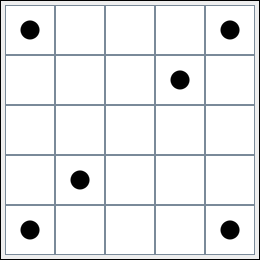
\includegraphics[width=3cm]{Figures/Chromosomes/6a.png} }}
            \qquad
            \subfloat{{
\includegraphics[width=3cm]{Figures/Chromosomes/6b.png} }}
            \caption{Optimal configurations of the small scale problem with 6 wind turbines using exhaustive search method, $obj=0.002004\;kW^{-1}$}
            \label{small6}
        \end{figure}
        
        The optimal solutions for a 1km by 1km win farm with 6 wind turbines found by exhaustive search is shown in Figure \ref{small6}. Both solution are just the same but differ only by a $90^o$ rotation of the whole wind farm. The power output of each wind turbine on the leftmost model in Figure \ref{small6} for different wind directions is shown in Table \ref{table6}.
        
        %INSERT TABLE6 HERE
        \singlespacing
        \begin{table}[H]
        	\centering
        	\begin{tabular}{|c|c|c|c|c|c|c|} \hline
        			& (0 0)		& (0 4)		& (1 3)		& (3 1)		& (4 0)		& (4 4)		\\ \hline
        		$0^o$	& 518.4kW	& 518.4kW	& 518.4kW	& 452.183kW	& 475.081kW	& 440.320kW	\\ \hline
        		$10^o$	& 518.4kW	& 518.4kW	& 518.4kW	& 518.4kW	& 474.053kW	& 474.053kW	\\ \hline
        		$20^o$	& 518.4kW	& 518.4kW	& 518.4kW	& 518.4kW	& 518.4kW	& 518.4kW	\\ \hline
        		$30^o$	& 518.4kW	& 518.4kW	& 347.609kW	& 433.294kW	& 342.660kW	& 518.4kW	\\ \hline
        		$40^o$	& 518.4kW	& 518.4kW	& 352.743kW	& 436.879kW	& 348.056kW	& 518.4kW	\\ \hline
        		$50^o$	& 518.4kW	& 518.4kW	& 352.743kW	& 436.879kW	& 348.056kW	& 518.4kW	\\ \hline
        		$60^o$	& 518.4kW	& 518.4kW	& 347.609kW	& 433.294kW	& 342.660kW	& 518.4kW	\\ \hline
        		$70^o$	& 518.4kW	& 518.4kW	& 518.4kW	& 518.4kW	& 518.4kW	& 518.4kW	\\ \hline
        		$80^o$	& 474.053kW	& 518.4kW	& 518.4kW	& 518.4kW	& 474.053kW	& 518.4kW	\\ \hline
        		$90^o$	& 440.320kW	& 518.4kW	& 518.4kW	& 452.183kW	& 475.081kW	& 518.4kW	\\ \hline
        		$100^o$	& 442.884kW	& 518.4kW	& 518.4kW	& 456.002kW	& 474.053kW	& 518.4kW	\\ \hline
        		$110^o$	& 456.934kW	& 518.4kW	& 518.4kW	& 456.934kW	& 518.4kW	& 518.4kW	\\ \hline
        		$120^o$	& 450.351kW	& 518.4kW	& 518.4kW	& 455.137kW	& 518.4kW	& 518.4kW	\\ \hline
        		$130^o$	& 493.350kW	& 518.4kW	& 518.4kW	& 518.4kW	& 518.4kW	& 518.4kW	\\ \hline
        		$140^o$	& 493.350kW	& 518.4kW	& 518.4kW	& 518.4kW	& 518.4kW	& 518.4kW	\\ \hline
        		$150^o$	& 450.351kW	& 518.4kW	& 455.137kW	& 518.4kW	& 518.4kW	& 518.4kW	\\ \hline
        		$160^o$	& 456.934kW	& 518.4kW	& 456.934kW	& 518.4kW	& 518.4kW	& 518.4kW	\\ \hline
        		$170^o$	& 442.884kW	& 474.053kW	& 456.002kW	& 518.4kW	& 518.4kW	& 518.4kW	\\ \hline
        		$180^o$	& 440.320kW	& 475.081kW	& 452.183kW	& 518.4kW	& 518.4kW	& 518.4kW	\\ \hline
        		$190^o$	& 474.053kW	& 474.053kW	& 518.4kW	& 518.4kW	& 518.4kW	& 518.4kW	\\ \hline
        		$200^o$	& 518.4kW	& 518.4kW	& 518.4kW	& 518.4kW	& 518.4kW	& 518.4kW	\\ \hline
        		$210^o$	& 518.4kW	& 342.660kW	& 433.294kW	& 347.609kW	& 518.4kW	& 518.4kW	\\ \hline
        		$220^o$	& 518.4kW	& 348.056kW	& 436.879kW	& 352.743kW	& 518.4kW	& 518.4kW	\\ \hline
        		$230^o$	& 518.4kW	& 348.056kW	& 436.879kW	& 352.743kW	& 518.4kW	& 518.4kW	\\ \hline
        		$240^o$	& 518.4kW	& 342.660kW	& 433.294kW	& 347.609kW	& 518.4kW	& 518.4kW	\\ \hline
        		$250^o$	& 518.4kW	& 518.4kW	& 518.4kW	& 518.4kW	& 518.4kW	& 518.4kW	\\ \hline
        		$260^o$	& 518.4kW	& 474.053kW	& 518.4kW	& 518.4kW	& 518.4kW	& 474.053kW	\\ \hline
        		$270^o$	& 518.4kW	& 475.081kW	& 452.183kW	& 518.4kW	& 518.4kW	& 440.320kW	\\ \hline
        		$280^o$	& 518.4kW	& 474.053kW	& 456.002kW	& 518.4kW	& 518.4kW	& 442.884kW	\\ \hline
        		$290^o$	& 518.4kW	& 518.4kW	& 456.934kW	& 518.4kW	& 518.4kW	& 456.934kW	\\ \hline
        		$300^o$	& 518.4kW	& 518.4kW	& 455.137kW	& 518.4kW	& 518.4kW	& 450.351kW	\\ \hline
        		$310^o$	& 518.4kW	& 518.4kW	& 518.4kW	& 518.4kW	& 518.4kW	& 493.350kW	\\ \hline
        		$320^o$	& 518.4kW	& 518.4kW	& 518.4kW	& 518.4kW	& 518.4kW	& 493.350kW	\\ \hline
        		$330^o$	& 518.4kW	& 518.4kW	& 518.4kW	& 455.137kW	& 518.4kW	& 450.351kW	\\ \hline
        		$340^o$	& 518.4kW	& 518.4kW	& 518.4kW	& 456.934kW	& 518.4kW	& 456.934kW	\\ \hline
        		$350^o$	& 518.4kW	& 518.4kW	& 518.4kW	& 456.002kW	& 474.053kW	& 442.884kW	\\ \hline
        	\end{tabular}
        	\caption{Power output of 6 wind turbines with optimal siting locations resulted from exhaustive search for different wind directions as shown in Figure \ref{small6}.}
        	\label{table6}
        \end{table}
        \doublespacing
        
        From Table \ref{table6}, the total annual power output of the whole wind farm is $2934.065kW$ which is $94.33\%$ of the theoretical maximum possible power output of a 1km by 1km wind farm with 6 wind turbines, with total cost of
        \begin{align*}
            Cost_{tot}
            &= N\left(\frac{2}{3} + \frac{1}{3}e^{-0.00174N^2}\right) \\
            &= \left(6\right)\left(\frac{2}{3} + \frac{1}{3}e^{-0.00174\left(6^2\right)}\right) \\
            &= 5.879
        \end{align*}
        Hence, the fitness of both chromosomes modelled in Figure \ref{small6} is
        \begin{align*}
            obj
            &=\frac{Cost_{tot}}{P_{tot}} \\
            &=\frac{5.879}{2934.065kW} \\
            &=0.002004kW^{-1}
        \end{align*}
        
    \textbf{G. 7 Wind Turbines}
        \begin{figure}[H]
            \centering
            \subfloat{{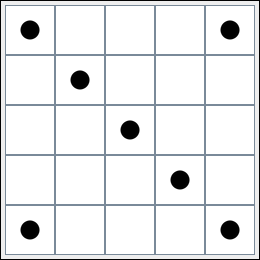
\includegraphics[width=3cm]{Figures/Chromosomes/7a.png} }}
            \qquad
            \subfloat{{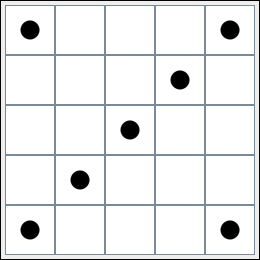
\includegraphics[width=3cm]{Figures/Chromosomes/7b.png} }}
            \caption{Optimal configurations of the small scale problem with 7 wind turbines using exhaustive search method, $obj=0.002025\;kW^{-1}$}
            \label{small7}
        \end{figure}
        
        The optimal solutions found by exhaustive search for a 1km by 1km wind farm wind 7 wind turbine are just the same as the optimal solutions with 6 wind turbines with an additional wind turbine at the center, as shown in Figure \ref{small7}. The power output of each wind turbine on the leftmost model in Figure \ref{small7} for different wind directions is shown in Table \ref{table7}.
        
        %INSERT TABLE7 HERE
        \singlespacing
        \begin{table}[H]
        	\centering
        	\begin{tabular}{|c|c|c|c|c|c|c|c|} \hline
        			& (0 0)		& (0 4)		& (1 1)		& (2 2)		& (3 3)		& (4 0)		& (4 4)		\\ \hline
        		$0^o$	& 518.4kW	& 518.4kW	& 518.4kW	& 518.4kW	& 452.183kW	& 440.320kW	& 475.081kW	\\ \hline
        		$10^o$	& 518.4kW	& 518.4kW	& 518.4kW	& 518.4kW	& 456.002kW	& 442.884kW	& 474.053kW	\\ \hline
        		$20^o$	& 518.4kW	& 518.4kW	& 518.4kW	& 518.4kW	& 456.934kW	& 456.934kW	& 518.4kW	\\ \hline
        		$30^o$	& 518.4kW	& 518.4kW	& 518.4kW	& 442.995kW	& 455.137kW	& 418.868kW	& 518.4kW	\\ \hline
        		$40^o$	& 518.4kW	& 518.4kW	& 518.4kW	& 446.124kW	& 518.4kW	& 442.374kW	& 518.4kW	\\ \hline
        		$50^o$	& 518.4kW	& 518.4kW	& 518.4kW	& 446.124kW	& 518.4kW	& 442.374kW	& 518.4kW	\\ \hline
        		$60^o$	& 518.4kW	& 518.4kW	& 455.137kW	& 442.995kW	& 518.4kW	& 418.868kW	& 518.4kW	\\ \hline
        		$70^o$	& 518.4kW	& 518.4kW	& 456.934kW	& 518.4kW	& 518.4kW	& 456.934kW	& 518.4kW	\\ \hline
        		$80^o$	& 474.053kW	& 518.4kW	& 456.002kW	& 518.4kW	& 518.4kW	& 442.884kW	& 518.4kW	\\ \hline
        		$90^o$	& 475.081kW	& 518.4kW	& 452.183kW	& 518.4kW	& 518.4kW	& 440.320kW	& 518.4kW	\\ \hline
        		$100^o$	& 474.053kW	& 518.4kW	& 518.4kW	& 518.4kW	& 518.4kW	& 474.053kW	& 518.4kW	\\ \hline
        		$110^o$	& 518.4kW	& 518.4kW	& 518.4kW	& 518.4kW	& 518.4kW	& 518.4kW	& 518.4kW	\\ \hline
        		$120^o$	& 331.294kW	& 518.4kW	& 332.538kW	& 335.781kW	& 347.609kW	& 518.4kW	& 518.4kW	\\ \hline
        		$130^o$	& 337.155kW	& 518.4kW	& 338.332kW	& 341.416kW	& 352.743kW	& 518.4kW	& 518.4kW	\\ \hline
        		$140^o$	& 337.155kW	& 518.4kW	& 338.332kW	& 341.416kW	& 352.743kW	& 518.4kW	& 518.4kW	\\ \hline
        		$150^o$	& 331.294kW	& 518.4kW	& 332.538kW	& 335.781kW	& 347.609kW	& 518.4kW	& 518.4kW	\\ \hline
        		$160^o$	& 518.4kW	& 518.4kW	& 518.4kW	& 518.4kW	& 518.4kW	& 518.4kW	& 518.4kW	\\ \hline
        		$170^o$	& 474.053kW	& 474.053kW	& 518.4kW	& 518.4kW	& 518.4kW	& 518.4kW	& 518.4kW	\\ \hline
        		$180^o$	& 475.081kW	& 440.320kW	& 452.183kW	& 518.4kW	& 518.4kW	& 518.4kW	& 518.4kW	\\ \hline
        		$190^o$	& 474.053kW	& 442.884kW	& 456.002kW	& 518.4kW	& 518.4kW	& 518.4kW	& 518.4kW	\\ \hline
        		$200^o$	& 518.4kW	& 456.934kW	& 456.934kW	& 518.4kW	& 518.4kW	& 518.4kW	& 518.4kW	\\ \hline
        		$210^o$	& 518.4kW	& 418.868kW	& 455.137kW	& 442.995kW	& 518.4kW	& 518.4kW	& 518.4kW	\\ \hline
        		$220^o$	& 518.4kW	& 442.374kW	& 518.4kW	& 446.124kW	& 518.4kW	& 518.4kW	& 518.4kW	\\ \hline
        		$230^o$	& 518.4kW	& 442.374kW	& 518.4kW	& 446.124kW	& 518.4kW	& 518.4kW	& 518.4kW	\\ \hline
        		$240^o$	& 518.4kW	& 418.868kW	& 518.4kW	& 442.995kW	& 455.137kW	& 518.4kW	& 518.4kW	\\ \hline
        		$250^o$	& 518.4kW	& 456.934kW	& 518.4kW	& 518.4kW	& 456.934kW	& 518.4kW	& 518.4kW	\\ \hline
        		$260^o$	& 518.4kW	& 442.884kW	& 518.4kW	& 518.4kW	& 456.002kW	& 518.4kW	& 474.053kW	\\ \hline
        		$270^o$	& 518.4kW	& 440.320kW	& 518.4kW	& 518.4kW	& 452.183kW	& 518.4kW	& 475.081kW	\\ \hline
        		$280^o$	& 518.4kW	& 474.053kW	& 518.4kW	& 518.4kW	& 518.4kW	& 518.4kW	& 474.053kW	\\ \hline
        		$290^o$	& 518.4kW	& 518.4kW	& 518.4kW	& 518.4kW	& 518.4kW	& 518.4kW	& 518.4kW	\\ \hline
        		$300^o$	& 518.4kW	& 518.4kW	& 347.609kW	& 335.781kW	& 332.538kW	& 518.4kW	& 331.294kW	\\ \hline
        		$310^o$	& 518.4kW	& 518.4kW	& 352.743kW	& 341.416kW	& 338.332kW	& 518.4kW	& 337.155kW	\\ \hline
        		$320^o$	& 518.4kW	& 518.4kW	& 352.743kW	& 341.416kW	& 338.332kW	& 518.4kW	& 337.155kW	\\ \hline
        		$330^o$	& 518.4kW	& 518.4kW	& 347.609kW	& 335.781kW	& 332.538kW	& 518.4kW	& 331.294kW	\\ \hline
        		$340^o$	& 518.4kW	& 518.4kW	& 518.4kW	& 518.4kW	& 518.4kW	& 518.4kW	& 518.4kW	\\ \hline
        		$350^o$	& 518.4kW	& 518.4kW	& 518.4kW	& 518.4kW	& 518.4kW	& 474.053kW	& 474.053kW	\\ \hline
        	\end{tabular}
        	\caption{Power output of 7 wind turbines with optimal siting locations resulted from exhaustive search for different wind directions as shown in Figure \ref{small7}.}
        	\label{table7}
        \end{table}
        \doublespacing
        
        From Table \ref{table7}, the total annual power output of the whole wind farm is $3362.319kW$ which is $92.66\%$ of the theoretical maximum possible power output of a 1km by 1km wind farm with 7 wind turbines, with total cost of
        \begin{align*}
            Cost_{tot}
            &= N\left(\frac{2}{3} + \frac{1}{3}e^{-0.00174N^2}\right) \\
            &= \left(7\right)\left(\frac{2}{3} + \frac{1}{3}e^{-0.00174\left(7^2\right)}\right) \\
            &= 6.809
        \end{align*}
        Hence, the fitness of both chromosomes modelled in Figure \ref{small7} is
        \begin{align*}
            obj
            &=\frac{Cost_{tot}}{P_{tot}} \\
            &=\frac{6.809}{3362.319kW} \\
            &=0.002025kW^{-1}
        \end{align*} 
        
    \textbf{H. 8 Wind Turbines}
        \begin{figure}[H]
            \centering
            \subfloat{{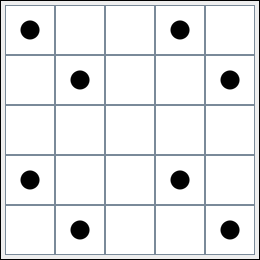
\includegraphics[width=3cm]{Figures/Chromosomes/8a.png} }}
            \qquad
            \subfloat{{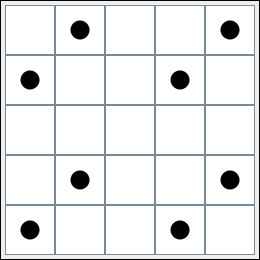
\includegraphics[width=3cm]{Figures/Chromosomes/8b.png} }}
            \caption{Optimal configurations of the small scale problem with 8 wind turbines using exhaustive search method, $obj=0.002044\;kW^{-1}$}
            \label{small8}
        \end{figure}
        
        As with the previous solutions for lower number of wind turbines, the optimal solutions for a 1km by 1km wind farm with 8 wind turbines shown in Figure \ref{small8} found by the exhaustive search are both same wind farm viewed from different angles. The power output of each wind turbine on the leftmost model in Figure \ref{small8} for different wind directions is shown in Tables \ref{table8a} and \ref{table8b}.
        
        %INSERT TABLE8 HERE
        \singlespacing
        \begin{table}[H]
        	\centering
        	\begin{tabular}{|c|c|c|c|c|} \hline
        			& (0 0)		& (0 3)		& (1 1)		& (1 4)			\\ \hline
        		$0^o$	& 518.4kW	& 518.4kW	& 518.4kW	& 518.4kW	\\ \hline
        		$10^o$	& 518.4kW	& 518.4kW	& 518.4kW	& 518.4kW	\\ \hline
        		$20^o$	& 518.4kW	& 518.4kW	& 518.4kW	& 518.4kW	\\ \hline
        		$30^o$	& 518.4kW	& 518.4kW	& 518.4kW	& 518.4kW	\\ \hline
        		$40^o$	& 518.4kW	& 518.4kW	& 518.4kW	& 518.4kW	\\ \hline
        		$50^o$	& 518.4kW	& 518.4kW	& 416.779kW	& 518.4kW	\\ \hline
        		$60^o$	& 518.4kW	& 518.4kW	& 420.036kW	& 518.4kW	\\ \hline
        		$70^o$	& 518.4kW	& 518.4kW	& 419.441kW	& 518.4kW	\\ \hline
        		$80^o$	& 450.741kW	& 518.4kW	& 397.374kW	& 518.4kW	\\ \hline
        		$90^o$	& 440.320kW	& 518.4kW	& 452.183kW	& 518.4kW	\\ \hline
        		$100^o$	& 440.028kW	& 518.4kW	& 450.741kW	& 518.4kW	\\ \hline
        		$110^o$	& 476.710kW	& 518.4kW	& 518.4kW	& 518.4kW	\\ \hline
        		$120^o$	& 338.852kW	& 347.609kW	& 433.294kW	& 518.4kW	\\ \hline
        		$130^o$	& 348.056kW	& 352.743kW	& 436.879kW	& 518.4kW	\\ \hline
        		$140^o$	& 348.056kW	& 352.743kW	& 436.879kW	& 518.4kW	\\ \hline
        		$150^o$	& 338.852kW	& 343.639kW	& 433.294kW	& 518.4kW	\\ \hline
        		$160^o$	& 476.710kW	& 476.710kW	& 518.4kW	& 518.4kW	\\ \hline
        		$170^o$	& 440.028kW	& 440.028kW	& 450.741kW	& 450.741kW	\\ \hline
        		$180^o$	& 440.320kW	& 440.320kW	& 452.183kW	& 452.183kW	\\ \hline
        		$190^o$	& 450.741kW	& 441.260kW	& 397.374kW	& 397.374kW	\\ \hline
        		$200^o$	& 518.4kW	& 481.608kW	& 419.441kW	& 419.441kW	\\ \hline
        		$210^o$	& 518.4kW	& 463.535kW	& 420.036kW	& 412.775kW	\\ \hline
        		$220^o$	& 518.4kW	& 463.947kW	& 416.779kW	& 410.417kW	\\ \hline
        		$230^o$	& 518.4kW	& 410.417kW	& 518.4kW	& 463.947kW	\\ \hline
        		$240^o$	& 518.4kW	& 412.775kW	& 518.4kW	& 463.535kW	\\ \hline
        		$250^o$	& 518.4kW	& 419.441kW	& 518.4kW	& 481.608kW	\\ \hline
        		$260^o$	& 518.4kW	& 397.374kW	& 518.4kW	& 441.260kW	\\ \hline
        		$270^o$	& 518.4kW	& 452.183kW	& 518.4kW	& 440.320kW	\\ \hline
        		$280^o$	& 518.4kW	& 450.741kW	& 518.4kW	& 440.028kW	\\ \hline
        		$290^o$	& 518.4kW	& 518.4kW	& 518.4kW	& 476.710kW	\\ \hline
        		$300^o$	& 518.4kW	& 518.4kW	& 347.609kW	& 343.639kW	\\ \hline
        		$310^o$	& 518.4kW	& 518.4kW	& 352.743kW	& 352.743kW	\\ \hline
        		$320^o$	& 518.4kW	& 518.4kW	& 352.743kW	& 352.743kW	\\ \hline
        		$330^o$	& 518.4kW	& 518.4kW	& 347.609kW	& 347.609kW	\\ \hline
        		$340^o$	& 518.4kW	& 518.4kW	& 518.4kW	& 518.4kW	\\ \hline
        		$350^o$	& 518.4kW	& 518.4kW	& 518.4kW	& 518.4kW	\\ \hline
        	\end{tabular}
        	\caption{Power output of 8 wind turbines with optimal siting locations resulted from exhaustive search for different wind directions as shown in Figure \ref{small8} (a).}
        	\label{table8a}
        \end{table}
        \begin{table}[H]
        	\centering
        	\begin{tabular}{|c|c|c|c|c|} \hline
        			& (3 0)		& (3 3)		& (4 1)		& (4 4)		\\ \hline
        		$0^o$	& 452.183kW	& 452.183kW	& 440.320kW	& 440.320kW	\\ \hline
        		$10^o$	& 397.374kW	& 397.374kW	& 441.260kW	& 450.741kW	\\ \hline
        		$20^o$	& 419.441kW	& 419.441kW	& 481.608kW	& 518.4kW	\\ \hline
        		$30^o$	& 412.775kW	& 420.036kW	& 463.535kW	& 518.4kW	\\ \hline
        		$40^o$	& 410.417kW	& 416.779kW	& 463.947kW	& 518.4kW	\\ \hline
        		$50^o$	& 463.947kW	& 518.4kW	& 410.417kW	& 518.4kW	\\ \hline
        		$60^o$	& 463.535kW	& 518.4kW	& 412.775kW	& 518.4kW	\\ \hline
        		$70^o$	& 481.608kW	& 518.4kW	& 419.441kW	& 518.4kW	\\ \hline
        		$80^o$	& 441.260kW	& 518.4kW	& 397.374kW	& 518.4kW	\\ \hline
        		$90^o$	& 440.320kW	& 518.4kW	& 452.183kW	& 518.4kW	\\ \hline
        		$100^o$	& 440.028kW	& 518.4kW	& 450.741kW	& 518.4kW	\\ \hline
        		$110^o$	& 476.710kW	& 518.4kW	& 518.4kW	& 518.4kW	\\ \hline
        		$120^o$	& 343.639kW	& 347.609kW	& 518.4kW	& 518.4kW	\\ \hline
        		$130^o$	& 352.743kW	& 352.743kW	& 518.4kW	& 518.4kW	\\ \hline
        		$140^o$	& 352.743kW	& 352.743kW	& 518.4kW	& 518.4kW	\\ \hline
        		$150^o$	& 347.609kW	& 347.609kW	& 518.4kW	& 518.4kW	\\ \hline
        		$160^o$	& 518.4kW	& 518.4kW	& 518.4kW	& 518.4kW	\\ \hline
        		$170^o$	& 518.4kW	& 518.4kW	& 518.4kW	& 518.4kW	\\ \hline
        		$180^o$	& 518.4kW	& 518.4kW	& 518.4kW	& 518.4kW	\\ \hline
        		$190^o$	& 518.4kW	& 518.4kW	& 518.4kW	& 518.4kW	\\ \hline
        		$200^o$	& 518.4kW	& 518.4kW	& 518.4kW	& 518.4kW	\\ \hline
        		$210^o$	& 518.4kW	& 518.4kW	& 518.4kW	& 518.4kW	\\ \hline
        		$220^o$	& 518.4kW	& 518.4kW	& 518.4kW	& 518.4kW	\\ \hline
        		$230^o$	& 518.4kW	& 416.779kW	& 518.4kW	& 518.4kW	\\ \hline
        		$240^o$	& 518.4kW	& 420.036kW	& 518.4kW	& 518.4kW	\\ \hline
        		$250^o$	& 518.4kW	& 419.441kW	& 518.4kW	& 518.4kW	\\ \hline
        		$260^o$	& 518.4kW	& 397.374kW	& 518.4kW	& 450.741kW	\\ \hline
        		$270^o$	& 518.4kW	& 452.183kW	& 518.4kW	& 440.320kW	\\ \hline
        		$280^o$	& 518.4kW	& 450.741kW	& 518.4kW	& 440.028kW	\\ \hline
        		$290^o$	& 518.4kW	& 518.4kW	& 518.4kW	& 476.710kW	\\ \hline
        		$300^o$	& 518.4kW	& 433.294kW	& 347.609kW	& 338.852kW	\\ \hline
        		$310^o$	& 518.4kW	& 436.879kW	& 352.743kW	& 348.056kW	\\ \hline
        		$320^o$	& 518.4kW	& 436.879kW	& 352.743kW	& 348.056kW	\\ \hline
        		$330^o$ & 518.4kW	& 433.294kW	& 343.639kW	& 338.852kW	\\ \hline
        		$340^o$	& 518.4kW	& 518.4kW	& 476.710kW	& 476.710kW	\\ \hline
        		$350^o$	& 450.741kW	& 450.741kW	& 440.028kW	& 440.028kW	\\ \hline
        	\end{tabular}
        	\caption{Power output of 8 wind turbines with optimal siting locations resulted from exhaustive search for different wind directions as shown in Figure \ref{small8} (b).}
        	\label{table8b}
        \end{table}
        \doublespacing
        
        From Tables \ref{table8a} and \ref{table8b}, the total annual power output of the whole wind farm is $3776.275kW$ which is $91.06\%$ of the theoretical maximum possible power output of a 1km by 1km wind farm with 8 wind turbines, with total cost of
        \begin{align*}
            Cost_{tot}
            &= N\left(\frac{2}{3} + \frac{1}{3}e^{-0.00174N^2}\right) \\
            &= \left(8\right)\left(\frac{2}{3} + \frac{1}{3}e^{-0.00174\left(8^2\right)}\right) \\
            &= 7.719
        \end{align*}
        Hence, the fitness of both chromosomes modelled in Figure \ref{small8} is
        \begin{align*}
            obj
            &=\frac{Cost_{tot}}{P_{tot}} \\
            &=\frac{7.719}{3776.275kW} \\
            &=0.002044kW^{-1}
        \end{align*} 
        
    \textbf{I. 9 Wind Turbines}
        \begin{figure}[H]
            \centering
            \subfloat{{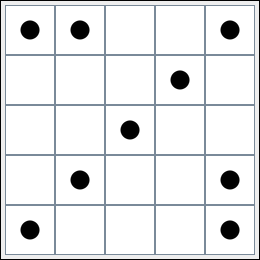
\includegraphics[width=3cm]{Figures/Chromosomes/9c.png} }}
            \qquad
            \subfloat{{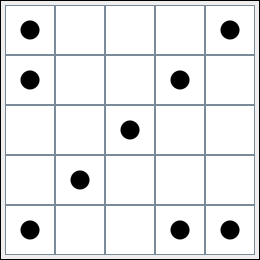
\includegraphics[width=3cm]{Figures/Chromosomes/9d.png} }}
            \qquad
            \subfloat{{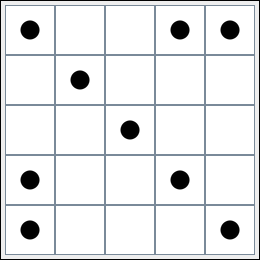
\includegraphics[width=3cm]{Figures/Chromosomes/9h.png} }}
            \qquad
            \subfloat{{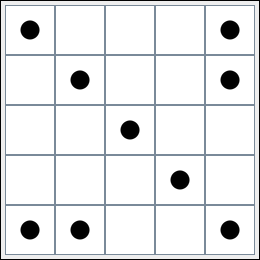
\includegraphics[width=3cm]{Figures/Chromosomes/9i.png} }}
            \caption{Optimal configurations of the small scale problem with 9 wind turbines using exhaustive search method, $obj=0.002066\;kW^{-1}$}
            \label{small9}
        \end{figure}
        
        Figure \ref{small9} shows the optimal configurations of a 1km by 1km wind farm win 9 wind turbines found by exhaustive search, where each wind farm shown in the figure are same wind farms rotated by $90^o$. The power output of each wind turbine on the leftmost model in Figure \ref{small9} for different wind directions is shown in Tables \ref{table9a} and \ref{table9b}.
        
        %INSERT TABLE9 HERE
        \singlespacing
        \begin{table}[H]
        	\centering
        	\begin{tabular}{|c|c|c|c|c|c|} \hline
        			& (0 0)		& (0 1)		& (0 4)		& (1 3)		& (2 2)		\\ \hline
        		$0^o$	& 518.4kW	& 518.4kW	& 518.4kW	& 518.4kW	& 518.4kW	\\ \hline
        		$10^o$	& 518.4kW	& 518.4kW	& 518.4kW	& 518.4kW	& 518.4kW	\\ \hline
        		$20^o$	& 518.4kW	& 518.4kW	& 518.4kW	& 518.4kW	& 518.4kW	\\ \hline
        		$30^o$	& 518.4kW	& 518.4kW	& 518.4kW	& 347.609kW	& 335.781kW	\\ \hline
        		$40^o$	& 518.4kW	& 518.4kW	& 518.4kW	& 352.743kW	& 341.416kW	\\ \hline
        		$50^o$	& 518.4kW	& 518.4kW	& 518.4kW	& 352.743kW	& 341.416kW	\\ \hline
        		$60^o$	& 518.4kW	& 518.4kW	& 518.4kW	& 347.609kW	& 335.781kW	\\ \hline
        		$70^o$	& 282.086kW	& 518.4kW	& 518.4kW	& 518.4kW	& 518.4kW	\\ \hline
        		$80^o$	& 287.903kW	& 450.741kW	& 518.4kW	& 518.4kW	& 518.4kW	\\ \hline
        		$90^o$	& 284.861kW	& 452.183kW	& 518.4kW	& 518.4kW	& 518.4kW	\\ \hline
        		$100^o$	& 282.834kW	& 397.374kW	& 518.4kW	& 518.4kW	& 414.911kW	\\ \hline
        		$110^o$	& 276.129kW	& 419.441kW	& 518.4kW	& 518.4kW	& 419.441kW	\\ \hline
        		$120^o$	& 414.941kW	& 412.775kW	& 518.4kW	& 518.4kW	& 397.367kW	\\ \hline
        		$130^o$	& 437.133kW	& 406.629kW	& 518.4kW	& 518.4kW	& 396.523kW	\\ \hline
        		$140^o$	& 436.702kW	& 406.922kW	& 518.4kW	& 416.779kW	& 446.124kW	\\ \hline
        		$150^o$	& 418.868kW	& 409.118kW	& 518.4kW	& 403.753kW	& 442.995kW	\\ \hline
        		$160^o$	& 456.934kW	& 414.993kW	& 518.4kW	& 404.128kW	& 518.4kW	\\ \hline
        		$170^o$	& 442.884kW	& 397.374kW	& 438.600kW	& 399.891kW	& 518.4kW	\\ \hline
        		$180^o$	& 440.320kW	& 440.320kW	& 440.320kW	& 452.183kW	& 518.4kW	\\ \hline
        		$190^o$	& 474.053kW	& 440.028kW	& 438.600kW	& 518.4kW	& 518.4kW	\\ \hline
        		$200^o$	& 518.4kW	& 476.710kW	& 518.4kW	& 518.4kW	& 518.4kW	\\ \hline
        		$210^o$	& 518.4kW	& 474.478kW	& 331.294kW	& 332.538kW	& 335.781kW	\\ \hline
        		$220^o$	& 518.4kW	& 518.4kW	& 337.155kW	& 338.332kW	& 341.416kW	\\ \hline
        		$230^o$	& 518.4kW	& 518.4kW	& 337.155kW	& 338.332kW	& 341.416kW	\\ \hline
        		$240^o$	& 518.4kW	& 518.4kW	& 331.294kW	& 332.538kW	& 335.781kW	\\ \hline
        		$250^o$	& 518.4kW	& 282.086kW	& 518.4kW	& 518.4kW	& 518.4kW	\\ \hline
        		$260^o$	& 518.4kW	& 290.474kW	& 438.600kW	& 518.4kW	& 518.4kW	\\ \hline
        		$270^o$	& 518.4kW	& 293.210kW	& 440.320kW	& 452.183kW	& 518.4kW	\\ \hline
        		$280^o$	& 518.4kW	& 290.474kW	& 438.600kW	& 399.891kW	& 518.4kW	\\ \hline
        		$290^o$	& 518.4kW	& 282.086kW	& 518.4kW	& 404.128kW	& 518.4kW	\\ \hline
        		$300^o$	& 518.4kW	& 518.4kW	& 518.4kW	& 403.753kW	& 442.995kW	\\ \hline
        		$310^o$	& 518.4kW	& 518.4kW	& 518.4kW	& 416.779kW	& 446.124kW	\\ \hline
        		$320^o$	& 518.4kW	& 518.4kW	& 518.4kW	& 518.4kW	& 396.523kW	\\ \hline
        		$330^o$	& 518.4kW	& 518.4kW	& 518.4kW	& 518.4kW	& 397.367kW	\\ \hline
        		$340^o$	& 518.4kW	& 518.4kW	& 518.4kW	& 518.4kW	& 419.441kW	\\ \hline
        		$350^o$	& 518.4kW	& 518.4kW	& 518.4kW	& 518.4kW	& 414.911kW	\\ \hline
        	\end{tabular}
        	\caption{Power output of 9 wind turbines with optimal siting locations resulted from exhaustive search for different wind directions as shown in Figure \ref{small9} (a).}
        	\label{table9a}
        \end{table}
        \begin{table}[H]
        	\centering
        	\begin{tabular}{|c|c|c|c|c|} \hline
        			& (3 1)		& (3 4)		& (4 0)		& (4 4)		\\ \hline
        		$0^o$	& 426.497kW	& 452.183kW	& 457.869kW	& 284.861kW	\\ \hline
        		$10^o$	& 450.741kW	& 450.741kW	& 458.379kW	& 287.903kW	\\ \hline
        		$20^o$	& 518.4kW	& 518.4kW	& 476.710kW	& 282.086kW	\\ \hline
        		$30^o$	& 332.538kW	& 518.4kW	& 327.826kW	& 518.4kW	\\ \hline
        		$40^o$	& 338.332kW	& 518.4kW	& 337.155kW	& 518.4kW	\\ \hline
        		$50^o$	& 338.332kW	& 518.4kW	& 337.155kW	& 518.4kW	\\ \hline
        		$60^o$	& 332.538kW	& 518.4kW	& 327.826kW	& 518.4kW	\\ \hline
        		$70^o$	& 518.4kW	& 518.4kW	& 476.710kW	& 518.4kW	\\ \hline
        		$80^o$	& 450.741kW	& 518.4kW	& 458.379kW	& 518.4kW	\\ \hline
        		$90^o$	& 426.497kW	& 518.4kW	& 457.869kW	& 518.4kW	\\ \hline
        		$100^o$	& 428.031kW	& 518.4kW	& 474.053kW	& 518.4kW	\\ \hline
        		$110^o$	& 456.934kW	& 518.4kW	& 518.4kW	& 518.4kW	\\ \hline
        		$120^o$	& 455.137kW	& 518.4kW	& 518.4kW	& 518.4kW	\\ \hline
        		$130^o$	& 518.4kW	& 518.4kW	& 518.4kW	& 518.4kW	\\ \hline
        		$140^o$	& 518.4kW	& 518.4kW	& 518.4kW	& 518.4kW	\\ \hline
        		$150^o$	& 518.4kW	& 518.4kW	& 518.4kW	& 518.4kW	\\ \hline
        		$160^o$	& 518.4kW	& 282.086kW	& 518.4kW	& 518.4kW	\\ \hline
        		$170^o$	& 518.4kW	& 290.474kW	& 518.4kW	& 518.4kW	\\ \hline
        		$180^o$	& 518.4kW	& 293.210kW	& 518.4kW	& 518.4kW	\\ \hline
        		$190^o$	& 518.4kW	& 290.474kW	& 518.4kW	& 518.4kW	\\ \hline
        		$200^o$	& 518.4kW	& 282.086kW	& 518.4kW	& 518.4kW	\\ \hline
        		$210^o$	& 347.609kW	& 518.4kW	& 518.4kW	& 518.4kW	\\ \hline
        		$220^o$	& 352.743kW	& 518.4kW	& 518.4kW	& 518.4kW	\\ \hline
        		$230^o$	& 352.743kW	& 518.4kW	& 518.4kW	& 518.4kW	\\ \hline
        		$240^o$	& 347.609kW	& 474.478kW	& 518.4kW	& 518.4kW	\\ \hline
        		$250^o$	& 518.4kW	& 476.710kW	& 518.4kW	& 518.4kW	\\ \hline
        		$260^o$	& 518.4kW	& 440.028kW	& 518.4kW	& 474.053kW	\\ \hline
        		$270^o$	& 518.4kW	& 440.320kW	& 518.4kW	& 440.320kW	\\ \hline
        		$280^o$	& 518.4kW	& 397.374kW	& 518.4kW	& 442.884kW	\\ \hline
        		$290^o$	& 518.4kW	& 414.993kW	& 518.4kW	& 456.934kW	\\ \hline
        		$300^o$	& 518.4kW	& 409.118kW	& 518.4kW	& 418.868kW	\\ \hline
        		$310^o$	& 518.4kW	& 406.922kW	& 518.4kW	& 436.702kW	\\ \hline
        		$320^o$	& 518.4kW	& 406.629kW	& 518.4kW	& 437.133kW	\\ \hline
        		$330^o$	& 455.137kW	& 412.775kW	& 518.4kW	& 414.941kW	\\ \hline
        		$340^o$	& 456.934kW	& 419.441kW	& 518.4kW	& 276.129kW	\\ \hline
        		$350^o$	& 428.031kW	& 397.374kW	& 474.053kW	& 282.834kW	\\ \hline
        	\end{tabular}
        	\caption{Power output of 9 wind turbines with optimal siting locations resulted from exhaustive search for different wind directions as shown in Figure \ref{small9} (b).}
        	\label{table9b}
        \end{table}
        \doublespacing
        
        From Tables \ref{table9a} and \ref{table9b}, the total annual power output of the whole wind farm is $4165.207kW$ which is $89.27\%$ of the theoretical maximum possible power output of a 1km by 1km wind farm with 9 wind turbines, with total cost of
        \begin{align*}
            Cost_{tot}
            &= N\left(\frac{2}{3} + \frac{1}{3}e^{-0.00174N^2}\right) \\
            &= \left(9\right)\left(\frac{2}{3} + \frac{1}{3}e^{-0.00174\left(9^2\right)}\right) \\
            &= 8.606
        \end{align*}
        Hence, the fitness of all chromosomes modelled in Figure \ref{small9} is
        \begin{align*}
            obj
            &=\frac{Cost_{tot}}{P_{tot}} \\
            &=\frac{8.606}{4165.207kW} \\
            &=0.002066kW^{-1}
        \end{align*} 
    
    \textbf{J. 10 Wind Turbines}
        \begin{figure}[H]
            \centering
            \subfloat{{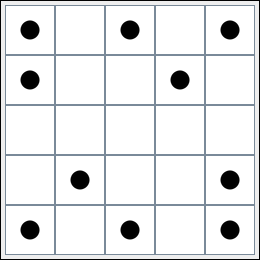
\includegraphics[width=3cm]{Figures/Chromosomes/10a.png} }}
            \qquad
            \subfloat{{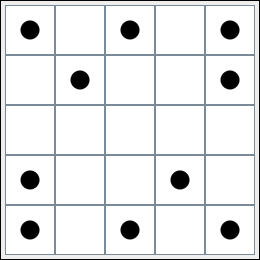
\includegraphics[width=3cm]{Figures/Chromosomes/10b.png} }}
            \qquad
            \subfloat{{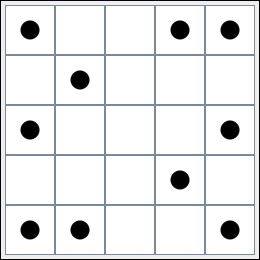
\includegraphics[width=3cm]{Figures/Chromosomes/10c.png} }}
            \qquad
            \subfloat{{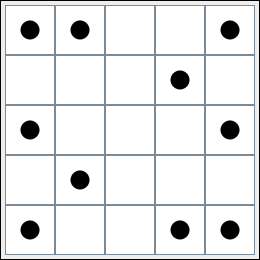
\includegraphics[width=3cm]{Figures/Chromosomes/10d.png} }}
            \caption{Optimal configurations of the small scale problem with 10 wind turbines using exhaustive search method, $obj=0.002082\;kW^{-1}$}
            \label{small10}
        \end{figure}
        
        From Figure \ref{small10}, all four chromosomes which are the optimal configurations of a 1km by 1km wind farm with 10 wind turbines found by exhaustive search, have the same annual total power output. The power output of each wind turbine on the leftmost model in Figure \ref{small10} for different wind directions is shown in Tables \ref{table10a} and \ref{table10b}.
        
        %INSERT TABLE10 HERE
        \singlespacing
        \begin{table}[H]
        	\centering
        	\begin{tabular}{|c|c|c|c|c|c|} \hline
        			& (0 0)		& (0 2)		& (0 4)		& (1 0)		& (1 3)		\\ \hline
        		$0^o$	& 518.4kW	& 518.4kW	& 518.4kW	& 293.210kW	& 518.4kW	\\ \hline
        		$10^o$	& 518.4kW	& 518.4kW	& 518.4kW	& 290.474kW	& 518.4kW	\\ \hline
        		$20^o$	& 518.4kW	& 518.4kW	& 518.4kW	& 282.086kW	& 518.4kW	\\ \hline
        		$30^o$	& 518.4kW	& 518.4kW	& 518.4kW	& 518.4kW	& 347.609kW	\\ \hline
        		$40^o$	& 518.4kW	& 518.4kW	& 518.4kW	& 518.4kW	& 352.743kW	\\ \hline
        		$50^o$	& 518.4kW	& 518.4kW	& 518.4kW	& 416.779kW	& 352.743kW	\\ \hline
        		$60^o$	& 518.4kW	& 518.4kW	& 518.4kW	& 412.007kW	& 347.609kW	\\ \hline
        		$70^o$	& 397.174kW	& 397.174kW	& 518.4kW	& 412.245kW	& 518.4kW	\\ \hline
        		$80^o$	& 396.867kW	& 403.702kW	& 518.4kW	& 391.766kW	& 518.4kW	\\ \hline
        		$90^o$	& 384.745kW	& 405.786kW	& 518.4kW	& 440.320kW	& 518.4kW	\\ \hline
        		$100^o$	& 384.346kW	& 403.702kW	& 518.4kW	& 441.260kW	& 518.4kW	\\ \hline
        		$110^o$	& 381.912kW	& 397.174kW	& 518.4kW	& 469.639kW	& 518.4kW	\\ \hline
        		$120^o$	& 444.339kW	& 347.609kW	& 518.4kW	& 471.045kW	& 518.4kW	\\ \hline
        		$130^o$	& 479.190kW	& 346.473kW	& 518.4kW	& 447.030kW	& 518.4kW	\\ \hline
        		$140^o$	& 463.666kW	& 344.144kW	& 518.4kW	& 402.728kW	& 416.779kW	\\ \hline
        		$150^o$	& 442.007kW	& 339.657kW	& 518.4kW	& 409.344kW	& 403.753kW	\\ \hline
        		$160^o$	& 275.789kW	& 454.672kW	& 518.4kW	& 407.968kW	& 404.128kW	\\ \hline
        		$170^o$	& 280.975kW	& 460.065kW	& 438.600kW	& 397.374kW	& 399.891kW	\\ \hline
        		$180^o$	& 284.861kW	& 440.320kW	& 440.320kW	& 452.183kW	& 426.497kW	\\ \hline
        		$190^o$	& 287.903kW	& 434.417kW	& 430.614kW	& 450.741kW	& 456.002kW	\\ \hline
        		$200^o$	& 282.086kW	& 447.560kW	& 481.608kW	& 518.4kW	& 456.934kW	\\ \hline
        		$210^o$	& 518.4kW	& 446.156kW	& 340.041kW	& 518.4kW	& 414.431kW	\\ \hline
        		$220^o$	& 518.4kW	& 480.364kW	& 345.079kW	& 518.4kW	& 436.879kW	\\ \hline
        		$230^o$	& 518.4kW	& 416.779kW	& 348.056kW	& 518.4kW	& 436.879kW	\\ \hline
        		$240^o$	& 518.4kW	& 420.036kW	& 338.852kW	& 518.4kW	& 433.294kW	\\ \hline
        		$250^o$	& 518.4kW	& 366.773kW	& 391.527kW	& 518.4kW	& 518.4kW	\\ \hline
        		$260^o$	& 518.4kW	& 368.786kW	& 391.288kW	& 518.4kW	& 450.741kW	\\ \hline
        		$270^o$	& 518.4kW	& 405.786kW	& 392.897kW	& 518.4kW	& 426.497kW	\\ \hline
        		$280^o$	& 518.4kW	& 403.702kW	& 396.867kW	& 518.4kW	& 428.031kW	\\ \hline
        		$290^o$	& 518.4kW	& 397.174kW	& 397.174kW	& 518.4kW	& 456.934kW	\\ \hline
        		$300^o$	& 518.4kW	& 518.4kW	& 518.4kW	& 518.4kW	& 339.303kW	\\ \hline
        		$310^o$	& 518.4kW	& 518.4kW	& 518.4kW	& 518.4kW	& 352.743kW	\\ \hline
        		$320^o$	& 518.4kW	& 518.4kW	& 518.4kW	& 518.4kW	& 352.743kW	\\ \hline
        		$330^o$	& 518.4kW	& 518.4kW	& 518.4kW	& 518.4kW	& 347.609kW	\\ \hline
        		$340^o$	& 518.4kW	& 518.4kW	& 518.4kW	& 282.086kW	& 518.4kW	\\ \hline
        		$350^o$	& 518.4kW	& 518.4kW	& 518.4kW	& 290.474kW	& 518.4kW	\\ \hline
        	\end{tabular}
        	\caption{Power output of 10 wind turbines with optimal siting locations resulted from exhaustive search for different wind directions as shown in Figure \ref{small10} (a).}
        	\label{table10a}
        \end{table}
        \begin{table}[H]
        	\centering
        	\begin{tabular}{|c|c|c|c|c|c|} \hline
        		& (3 1)		& (3 4)		& (4 0)		& (4 2)		& (4 4)		\\ \hline
        		$0^o$	& 426.497kW	& 452.183kW	& 440.320kW	& 440.320kW	& 284.861kW	\\ \hline
        		$10^o$	& 456.002kW	& 450.741kW	& 430.614kW	& 434.417kW	& 287.903kW	\\ \hline
        		$20^o$	& 456.934kW	& 518.4kW	& 481.608kW	& 447.560kW	& 282.086kW	\\ \hline
        		$30^o$	& 414.431kW	& 518.4kW	& 340.041kW	& 446.156kW	& 518.4kW	\\ \hline
        		$40^o$	& 436.879kW	& 518.4kW	& 345.079kW	& 480.364kW	& 518.4kW	\\ \hline
        		$50^o$	& 436.879kW	& 518.4kW	& 348.056kW	& 416.779kW	& 518.4kW	\\ \hline
        		$60^o$	& 433.294kW	& 518.4kW	& 338.852kW	& 420.036kW	& 518.4kW	\\ \hline
        		$70^o$	& 518.4kW	& 518.4kW	& 391.527kW	& 366.773kW	& 518.4kW	\\ \hline
        		$80^o$	& 450.741kW	& 518.4kW	& 391.288kW	& 368.786kW	& 518.4kW	\\ \hline
        		$90^o$	& 426.497kW	& 518.4kW	& 392.897kW	& 405.786kW	& 518.4kW	\\ \hline
        		$100^o$	& 428.031kW	& 518.4kW	& 396.867kW	& 403.702kW	& 518.4kW	\\ \hline
        		$110^o$	& 456.934kW	& 518.4kW	& 397.174kW	& 397.174kW	& 518.4kW	\\ \hline
        		$120^o$	& 339.303kW	& 518.4kW	& 518.4kW	& 518.4kW	& 518.4kW	\\ \hline
        		$130^o$	& 352.743kW	& 518.4kW	& 518.4kW	& 518.4kW	& 518.4kW	\\ \hline
        		$140^o$	& 352.743kW	& 518.4kW	& 518.4kW	& 518.4kW	& 518.4kW	\\ \hline
        		$150^o$	& 347.609kW	& 518.4kW	& 518.4kW	& 518.4kW	& 518.4kW	\\ \hline
        		$160^o$	& 518.4kW	& 282.086kW	& 518.4kW	& 518.4kW	& 518.4kW	\\ \hline
        		$170^o$	& 518.4kW	& 290.474kW	& 518.4kW	& 518.4kW	& 518.4kW	\\ \hline
        		$180^o$	& 518.4kW	& 293.210kW	& 518.4kW	& 518.4kW	& 518.4kW	\\ \hline
        		$190^o$	& 518.4kW	& 290.474kW	& 518.4kW	& 518.4kW	& 518.4kW	\\ \hline
        		$200^o$	& 518.4kW	& 282.086kW	& 518.4kW	& 518.4kW	& 518.4kW	\\ \hline
        		$210^o$	& 347.609kW	& 518.4kW	& 518.4kW	& 518.4kW	& 518.4kW	\\ \hline
        		$220^o$	& 352.743kW	& 518.4kW	& 518.4kW	& 518.4kW	& 518.4kW	\\ \hline
        		$230^o$	& 352.743kW	& 416.779kW	& 518.4kW	& 518.4kW	& 518.4kW	\\ \hline
        		$240^o$	& 347.609kW	& 412.007kW	& 518.4kW	& 518.4kW	& 518.4kW	\\ \hline
        		$250^o$	& 518.4kW	& 412.245kW	& 518.4kW	& 397.174kW	& 397.174kW	\\ \hline
        		$260^o$	& 518.4kW	& 391.766kW	& 518.4kW	& 403.702kW	& 396.867kW	\\ \hline
        		$270^o$	& 518.4kW	& 440.320kW	& 518.4kW	& 405.786kW	& 384.745kW	\\ \hline
        		$280^o$	& 518.4kW	& 441.260kW	& 518.4kW	& 403.702kW	& 384.346kW	\\ \hline
        		$290^o$	& 518.4kW	& 469.639kW	& 518.4kW	& 397.174kW	& 381.912kW	\\ \hline
        		$300^o$	& 518.4kW	& 471.045kW	& 518.4kW	& 347.609kW	& 444.339kW	\\ \hline
        		$310^o$	& 518.4kW	& 447.030kW	& 518.4kW	& 346.473kW	& 479.190kW	\\ \hline
        		$320^o$	& 416.779kW	& 402.728kW	& 518.4kW	& 344.144kW	& 463.666kW	\\ \hline
        		$330^o$	& 403.753kW	& 409.344kW	& 518.4kW	& 339.657kW	& 442.007kW	\\ \hline
        		$340^o$	& 404.128kW	& 407.968kW	& 518.4kW	& 454.672kW	& 275.789kW	\\ \hline
        		$350^o$	& 399.891kW	& 397.374kW	& 438.600kW	& 460.065kW	& 280.975kW	\\ \hline
        	\end{tabular}
        	\caption{Power output of 10 wind turbines with optimal siting locations resulted from exhaustive search for different wind directions as shown in Figure \ref{small10} (b).}
        	\label{table10b}
        \end{table}
        \doublespacing
        
        From Tables \ref{table10a} and \ref{table10b}, the total annual power output of the whole wind farm is $4547.176kW$ which is $87.72\%$ of the theoretical maximum possible power output of a 1km by 1km wind farm with 10 wind turbines, with total cost of
        \begin{align*}
            Cost_{tot}
            &= N\left(\frac{2}{3} + \frac{1}{3}e^{-0.00174N^2}\right) \\
            &= \left(10\right)\left(\frac{2}{3} + \frac{1}{3}e^{-0.00174\left(10^2\right)}\right) \\
            &= 9.468
        \end{align*}
        Hence, the fitness of all chromosomes modelled in Figure \ref{small10} is
        \begin{align*}
            obj
            &=\frac{Cost_{tot}}{P_{tot}} \\
            &=\frac{9.468}{4547.176kW} \\
            &=0.002082kW^{-1}
        \end{align*} 
        
    \textbf{K. 11 Wind Turbines}
        \begin{figure}[H]
            \centering
            \subfloat{{
\includegraphics[width=3cm]{Figures/Chromosomes/11a.png} }}
            \qquad
            \subfloat{{
\includegraphics[width=3cm]{Figures/Chromosomes/11b.png} }}
            \qquad
            \subfloat{{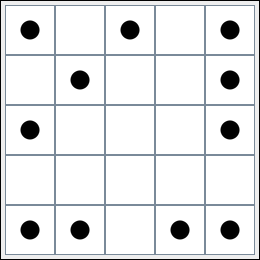
\includegraphics[width=3cm]{Figures/Chromosomes/11c.png} }}
            \qquad
            \subfloat{{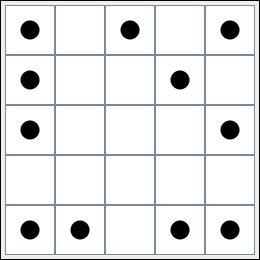
\includegraphics[width=3cm]{Figures/Chromosomes/11d.png} }}
            \qquad
            \subfloat{{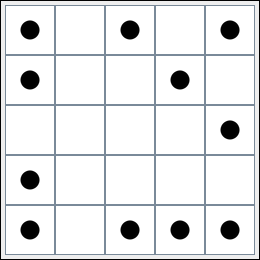
\includegraphics[width=3cm]{Figures/Chromosomes/11e.png} }}
            \qquad
            \subfloat{{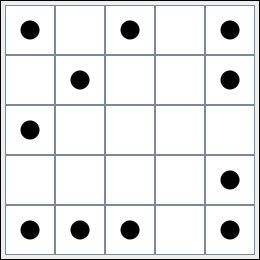
\includegraphics[width=3cm]{Figures/Chromosomes/11f.png} }}
            \qquad
            \subfloat{{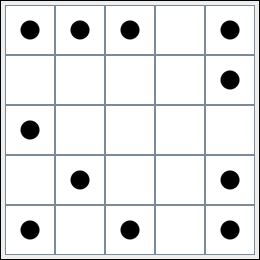
\includegraphics[width=3cm]{Figures/Chromosomes/11g.png} }}
            \qquad
            \subfloat{{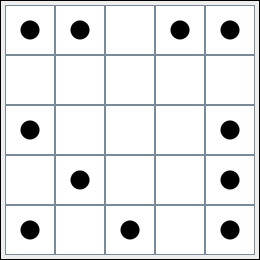
\includegraphics[width=3cm]{Figures/Chromosomes/11h.png} }}
            \caption{Optimal configurations of the small scale problem with 11 wind turbines using exhaustive search method, $obj=0.002095$}
            \label{small11}
        \end{figure}
        
        For 11 wind turbines on a 1km by 1km wind farm, the exhaustive search found 8 optimal configurations as shown in Figure \ref{small11}. The power output of each wind turbine on the leftmost model in Figure \ref{small11} for different wind directions is shown in Tables \ref{table11a} and \ref{table11b}.
        
        %INSERT TABLE11 HERE
        \singlespacing
        \begin{table}[H]
        	\centering
        	\begin{tabular}{|c|c|c|c|c|c|c|} \hline
        			& (0 0)		& (0 1)		& (0 3)		& (0 4)		& (2 0)		& (2 4)		\\ \hline
        		$0^o$	& 518.4kW	& 518.4kW	& 518.4kW	& 518.4kW	& 405.786kW	& 405.786kW	\\ \hline
        		$10^o$	& 518.4kW	& 518.4kW	& 518.4kW	& 518.4kW	& 368.786kW	& 403.702kW	\\ \hline
        		$20^o$	& 518.4kW	& 518.4kW	& 518.4kW	& 518.4kW	& 366.773kW	& 397.174kW	\\ \hline
        		$30^o$	& 518.4kW	& 518.4kW	& 518.4kW	& 518.4kW	& 420.036kW	& 518.4kW	\\ \hline
        		$40^o$	& 518.4kW	& 518.4kW	& 518.4kW	& 518.4kW	& 405.240kW	& 518.4kW	\\ \hline
        		$50^o$	& 518.4kW	& 518.4kW	& 518.4kW	& 518.4kW	& 455.385kW	& 518.4kW	\\ \hline
        		$60^o$	& 518.4kW	& 518.4kW	& 518.4kW	& 518.4kW	& 456.488kW	& 518.4kW	\\ \hline
        		$70^o$	& 282.086kW	& 397.174kW	& 282.086kW	& 518.4kW	& 454.672kW	& 518.4kW	\\ \hline
        		$80^o$	& 281.919kW	& 388.033kW	& 290.474kW	& 518.4kW	& 460.065kW	& 518.4kW	\\ \hline
        		$90^o$	& 284.861kW	& 390.444kW	& 293.210kW	& 518.4kW	& 440.320kW	& 518.4kW	\\ \hline
        		$100^o$	& 280.074kW	& 388.033kW	& 290.474kW	& 518.4kW	& 434.417kW	& 518.4kW	\\ \hline
        		$110^o$	& 280.437kW	& 388.099kW	& 282.086kW	& 518.4kW	& 447.560kW	& 518.4kW	\\ \hline
        		$120^o$	& 457.987kW	& 467.548kW	& 518.4kW	& 518.4kW	& 416.149kW	& 518.4kW	\\ \hline
        		$130^o$	& 458.881kW	& 439.275kW	& 518.4kW	& 518.4kW	& 437.644kW	& 518.4kW	\\ \hline
        		$140^o$	& 458.881kW	& 439.723kW	& 416.779kW	& 518.4kW	& 446.124kW	& 518.4kW	\\ \hline
        		$150^o$	& 457.987kW	& 445.895kW	& 412.007kW	& 518.4kW	& 442.995kW	& 518.4kW	\\ \hline
        		$160^o$	& 392.776kW	& 444.972kW	& 412.245kW	& 397.174kW	& 263.136kW	& 397.174kW	\\ \hline
        		$170^o$	& 377.959kW	& 476.899kW	& 391.766kW	& 396.867kW	& 272.511kW	& 403.702kW	\\ \hline
        		$180^o$	& 384.745kW	& 430.269kW	& 430.269kW	& 384.745kW	& 275.565kW	& 405.786kW	\\ \hline
        		$190^o$	& 382.200kW	& 394.135kW	& 440.028kW	& 380.016kW	& 272.511kW	& 403.702kW	\\ \hline
        		$200^o$	& 397.174kW	& 398.056kW	& 465.930kW	& 381.090kW	& 263.136kW	& 397.174kW	\\ \hline
        		$210^o$	& 518.4kW	& 397.044kW	& 451.663kW	& 442.007kW	& 518.4kW	& 335.781kW	\\ \hline
        		$220^o$	& 518.4kW	& 416.779kW	& 446.148kW	& 463.666kW	& 518.4kW	& 341.416kW	\\ \hline
        		$230^o$	& 518.4kW	& 518.4kW	& 447.565kW	& 464.352kW	& 518.4kW	& 338.600kW	\\ \hline
        		$240^o$	& 518.4kW	& 518.4kW	& 453.432kW	& 464.625kW	& 518.4kW	& 329.782kW	\\ \hline
        		$250^o$	& 518.4kW	& 282.086kW	& 388.099kW	& 279.157kW	& 518.4kW	& 463.389kW	\\ \hline
        		$260^o$	& 518.4kW	& 290.474kW	& 388.033kW	& 280.074kW	& 518.4kW	& 447.713kW	\\ \hline
        		$270^o$	& 518.4kW	& 293.210kW	& 390.444kW	& 284.861kW	& 518.4kW	& 457.869kW	\\ \hline
        		$280^o$	& 518.4kW	& 290.474kW	& 388.033kW	& 281.919kW	& 518.4kW	& 460.065kW	\\ \hline
        		$290^o$	& 518.4kW	& 282.086kW	& 397.174kW	& 282.086kW	& 518.4kW	& 454.672kW	\\ \hline
        		$300^o$	& 518.4kW	& 518.4kW	& 518.4kW	& 518.4kW	& 518.4kW	& 456.488kW	\\ \hline
        		$310^o$	& 518.4kW	& 518.4kW	& 518.4kW	& 518.4kW	& 518.4kW	& 455.385kW	\\ \hline
        		$320^o$	& 518.4kW	& 518.4kW	& 518.4kW	& 518.4kW	& 518.4kW	& 405.240kW	\\ \hline
        		$330^o$	& 518.4kW	& 518.4kW	& 518.4kW	& 518.4kW	& 518.4kW	& 420.036kW	\\ \hline
        		$340^o$	& 518.4kW	& 518.4kW	& 518.4kW	& 518.4kW	& 397.174kW	& 366.773kW	\\ \hline
        		$350^o$	& 518.4kW	& 518.4kW	& 518.4kW	& 518.4kW	& 403.702kW	& 368.786kW	\\ \hline
        	\end{tabular}
        	\caption{Power output of 11 wind turbines with optimal siting locations resulted from exhaustive search for different wind directions as shown in Figure \ref{small11} (a).}
        	\label{table11a}
        \end{table}
        \begin{table}[H]
        	\centering
        	\begin{tabular}{|c|c|c|c|c|c|} \hline
        			& (3 0)		& (3 3)		& (4 0)		& (4 2)		& (4 4)		\\ \hline
        		$0^o$	& 281.555kW	& 426.497kW	& 271.221kW	& 457.869kW	& 392.897kW	\\ \hline
        		$10^o$	& 279.437kW	& 428.031kW	& 268.338kW	& 462.133kW	& 396.867kW	\\ \hline
        		$20^o$	& 277.380kW	& 456.934kW	& 260.183kW	& 463.389kW	& 397.174kW	\\ \hline
        		$30^o$	& 443.577kW	& 339.303kW	& 459.513kW	& 329.782kW	& 518.4kW	\\ \hline
        		$40^o$	& 467.952kW	& 352.743kW	& 479.190kW	& 338.600kW	& 518.4kW	\\ \hline
        		$50^o$	& 468.703kW	& 352.743kW	& 463.666kW	& 341.416kW	& 518.4kW	\\ \hline
        		$60^o$	& 451.663kW	& 347.609kW	& 442.007kW	& 335.781kW	& 518.4kW	\\ \hline
        		$70^o$	& 465.930kW	& 518.4kW	& 381.090kW	& 397.174kW	& 518.4kW	\\ \hline
        		$80^o$	& 440.028kW	& 518.4kW	& 380.016kW	& 403.702kW	& 518.4kW	\\ \hline
        		$90^o$	& 430.269kW	& 518.4kW	& 384.745kW	& 405.786kW	& 518.4kW	\\ \hline
        		$100^o$	& 391.766kW	& 518.4kW	& 396.867kW	& 403.702kW	& 518.4kW	\\ \hline
        		$110^o$	& 412.245kW	& 518.4kW	& 397.174kW	& 397.174kW	& 518.4kW	\\ \hline
        		$120^o$	& 412.007kW	& 347.609kW	& 518.4kW	& 518.4kW	& 518.4kW	\\ \hline
        		$130^o$	& 416.779kW	& 352.743kW	& 518.4kW	& 518.4kW	& 518.4kW	\\ \hline
        		$140^o$	& 518.4kW	& 352.743kW	& 518.4kW	& 518.4kW	& 518.4kW	\\ \hline
        		$150^o$	& 518.4kW	& 347.609kW	& 518.4kW	& 518.4kW	& 518.4kW	\\ \hline
        		$160^o$	& 282.086kW	& 518.4kW	& 518.4kW	& 518.4kW	& 518.4kW	\\ \hline
        		$170^o$	& 290.474kW	& 518.4kW	& 518.4kW	& 518.4kW	& 518.4kW	\\ \hline
        		$180^o$	& 293.210kW	& 518.4kW	& 518.4kW	& 518.4kW	& 518.4kW	\\ \hline
        		$190^o$	& 290.474kW	& 518.4kW	& 518.4kW	& 518.4kW	& 518.4kW	\\ \hline
        		$200^o$	& 282.086kW	& 518.4kW	& 518.4kW	& 518.4kW	& 518.4kW	\\ \hline
        		$210^o$	& 518.4kW	& 347.609kW	& 518.4kW	& 518.4kW	& 518.4kW	\\ \hline
        		$220^o$	& 518.4kW	& 352.743kW	& 518.4kW	& 518.4kW	& 518.4kW	\\ \hline
        		$230^o$	& 518.4kW	& 352.743kW	& 518.4kW	& 518.4kW	& 518.4kW	\\ \hline
        		$240^o$	& 518.4kW	& 339.303kW	& 518.4kW	& 518.4kW	& 518.4kW	\\ \hline
        		$250^o$	& 518.4kW	& 456.934kW	& 518.4kW	& 397.174kW	& 397.174kW	\\ \hline
        		$260^o$	& 518.4kW	& 428.031kW	& 518.4kW	& 403.702kW	& 396.867kW	\\ \hline
        		$270^o$	& 518.4kW	& 407.461kW	& 518.4kW	& 405.786kW	& 392.897kW	\\ \hline
        		$280^o$	& 518.4kW	& 428.031kW	& 518.4kW	& 368.786kW	& 386.652kW	\\ \hline
        		$290^o$	& 518.4kW	& 456.934kW	& 518.4kW	& 366.773kW	& 387.374kW	\\ \hline
        		$300^o$	& 518.4kW	& 443.577kW	& 518.4kW	& 397.367kW	& 339.663kW	\\ \hline
        		$310^o$	& 518.4kW	& 452.230kW	& 518.4kW	& 396.523kW	& 346.271kW	\\ \hline
        		$320^o$	& 518.4kW	& 454.370kW	& 518.4kW	& 437.644kW	& 349.447kW	\\ \hline
        		$330^o$	& 518.4kW	& 453.432kW	& 518.4kW	& 425.807kW	& 340.422kW	\\ \hline
        		$340^o$	& 282.086kW	& 465.486kW	& 263.136kW	& 463.389kW	& 388.250kW	\\ \hline
        		$350^o$	& 284.374kW	& 450.741kW	& 270.266kW	& 462.133kW	& 391.288kW	\\ \hline
        	\end{tabular}
        	\caption{Power output of 11 wind turbines with optimal siting locations resulted from exhaustive search for different wind directions as shown in Figure \ref{small11} (b).}
        	\label{table11b}
        \end{table}
        \doublespacing
        
        From Tables \ref{table11a} and \ref{table11b}, the total annual power output of the whole wind farm is $4918.085kW$ which is $86.25\%$ of the theoretical maximum possible power output of a 1km by 1km wind farm with 11 wind turbines, with total cost of
        \begin{align*}
            Cost_{tot}
            &= N\left(\frac{2}{3} + \frac{1}{3}e^{-0.00174N^2}\right) \\
            &= \left(11\right)\left(\frac{2}{3} + \frac{1}{3}e^{-0.00174\left(11^2\right)}\right) \\
            &=10.304
        \end{align*}
        Hence, the fitness of all chromosomes modelled in Figure \ref{small11} is
        \begin{align*}
            obj
            &=\frac{Cost_{tot}}{P_{tot}} \\
            &=\frac{10.304}{4918.085kW} \\
            &=0.002095kW^{-1}
        \end{align*} 
        
    \textbf{L. 12 Wind Turbines}
        \begin{figure}[H]
            \centering
            \subfloat{{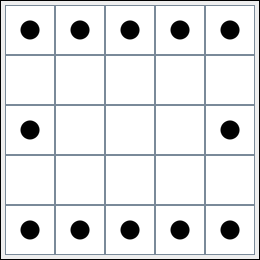
\includegraphics[width=3cm]{Figures/Chromosomes/12a.png} }}
            \qquad
            \subfloat{{
\includegraphics[width=3cm]{Figures/Chromosomes/12b.png} }}
            \caption{Optimal configurations of the small scale problem with 12 wind turbines using exhaustive search method, $obj=0.002101\;kW^{-1}$}
            \label{small12}
        \end{figure}
        
        Figure \ref{small12} shows two optimal configuration of a 1km by 1km wind farm with 12 wind turbines found by exhaustive search. The power output of each wind turbine on the leftmost model in Figure \ref{small12} for different wind directions is shown in Tables \ref{table12a} and \ref{table12b}.
        
        %INSERT TABLE12 HERE
        \singlespacing
        \begin{table}[H]
        	\centering
        	\begin{tabular}{|c|c|c|c|c|c|c|} \hline
        			& (0 0)		& (0 1)		& (0 2)		& (0 3)		& (0 4)		& (2 0)		\\ \hline
        		$0^o$	& 518.4kW	& 518.4kW	& 518.4kW	& 518.4kW	& 518.4kW	& 405.786kW	\\ \hline
        		$10^o$	& 518.4kW	& 518.4kW	& 518.4kW	& 518.4kW	& 518.4kW	& 368.786kW	\\ \hline
        		$20^o$	& 518.4kW	& 518.4kW	& 518.4kW	& 518.4kW	& 518.4kW	& 366.773kW	\\ \hline
        		$30^o$	& 518.4kW	& 518.4kW	& 518.4kW	& 518.4kW	& 518.4kW	& 397.367kW	\\ \hline
        		$40^o$	& 518.4kW	& 518.4kW	& 518.4kW	& 518.4kW	& 518.4kW	& 387.178kW	\\ \hline
        		$50^o$	& 518.4kW	& 518.4kW	& 518.4kW	& 518.4kW	& 518.4kW	& 424.308kW	\\ \hline
        		$60^o$	& 518.4kW	& 518.4kW	& 518.4kW	& 518.4kW	& 518.4kW	& 422.662kW	\\ \hline
        		$70^o$	& 263.136kW	& 263.136kW	& 263.136kW	& 282.086kW	& 518.4kW	& 454.672kW	\\ \hline
        		$80^o$	& 265.017kW	& 267.174kW	& 272.511kW	& 290.474kW	& 518.4kW	& 460.065kW	\\ \hline
        		$90^o$	& 268.237kW	& 270.342kW	& 275.565kW	& 293.210kW	& 518.4kW	& 475.081kW	\\ \hline
        		$100^o$	& 263.391kW	& 267.174kW	& 272.511kW	& 290.474kW	& 518.4kW	& 460.065kW	\\ \hline
        		$110^o$	& 261.707kW	& 260.131kW	& 263.136kW	& 282.086kW	& 518.4kW	& 454.672kW	\\ \hline
        		$120^o$	& 473.721kW	& 467.548kW	& 442.995kW	& 518.4kW	& 518.4kW	& 422.662kW	\\ \hline
        		$130^o$	& 463.666kW	& 458.745kW	& 446.124kW	& 518.4kW	& 518.4kW	& 424.308kW	\\ \hline
        		$140^o$	& 464.352kW	& 447.030kW	& 437.644kW	& 416.779kW	& 518.4kW	& 387.178kW	\\ \hline
        		$150^o$	& 449.876kW	& 454.622kW	& 425.807kW	& 412.007kW	& 518.4kW	& 397.367kW	\\ \hline
        		$160^o$	& 384.231kW	& 455.032kW	& 463.389kW	& 412.245kW	& 397.174kW	& 366.773kW	\\ \hline
        		$170^o$	& 386.652kW	& 447.713kW	& 447.713kW	& 400.973kW	& 396.867kW	& 368.786kW	\\ \hline
        		$180^o$	& 392.897kW	& 444.948kW	& 444.948kW	& 444.948kW	& 392.897kW	& 405.786kW	\\ \hline
        		$190^o$	& 396.867kW	& 400.973kW	& 447.713kW	& 447.713kW	& 386.652kW	& 403.702kW	\\ \hline
        		$200^o$	& 397.174kW	& 412.245kW	& 463.389kW	& 455.032kW	& 384.231kW	& 397.174kW	\\ \hline
        		$210^o$	& 518.4kW	& 412.007kW	& 425.807kW	& 454.622kW	& 449.876kW	& 518.4kW	\\ \hline
        		$220^o$	& 518.4kW	& 416.779kW	& 437.644kW	& 447.030kW	& 464.352kW	& 518.4kW	\\ \hline
        		$230^o$	& 518.4kW	& 518.4kW	& 446.124kW	& 458.745kW	& 463.666kW	& 518.4kW	\\ \hline
        		$240^o$	& 518.4kW	& 518.4kW	& 442.995kW	& 467.548kW	& 473.721kW	& 518.4kW	\\ \hline
        		$250^o$	& 518.4kW	& 282.086kW	& 263.136kW	& 260.131kW	& 261.707kW	& 518.4kW	\\ \hline
        		$260^o$	& 518.4kW	& 290.474kW	& 272.511kW	& 267.174kW	& 263.391kW	& 518.4kW	\\ \hline
        		$270^o$	& 518.4kW	& 293.210kW	& 275.565kW	& 270.342kW	& 268.237kW	& 518.4kW	\\ \hline
        		$280^o$	& 518.4kW	& 290.474kW	& 272.511kW	& 267.174kW	& 265.017kW	& 518.4kW	\\ \hline
        		$290^o$	& 518.4kW	& 282.086kW	& 263.136kW	& 263.136kW	& 263.136kW	& 518.4kW	\\ \hline
        		$300^o$	& 518.4kW	& 518.4kW	& 518.4kW	& 518.4kW	& 518.4kW	& 518.4kW	\\ \hline
        		$310^o$	& 518.4kW	& 518.4kW	& 518.4kW	& 518.4kW	& 518.4kW	& 518.4kW	\\ \hline
        		$320^o$	& 518.4kW	& 518.4kW	& 518.4kW	& 518.4kW	& 518.4kW	& 518.4kW	\\ \hline
        		$330^o$	& 518.4kW	& 518.4kW	& 518.4kW	& 518.4kW	& 518.4kW	& 518.4kW	\\ \hline
        		$340^o$	& 518.4kW	& 518.4kW	& 518.4kW	& 518.4kW	& 518.4kW	& 397.174kW	\\ \hline
        		$350^o$	& 518.4kW	& 518.4kW	& 518.4kW	& 518.4kW	& 518.4kW	& 403.702kW	\\ \hline
        	\end{tabular}
        	\caption{Power output of 12 wind turbines with optimal siting locations resulted from exhaustive search for different wind directions as shown in Figure \ref{small12} (a).}
        	\label{table12a}
        \end{table}
        \begin{table}[H]
        	\centering
        	\begin{tabular}{|c|c|c|c|c|c|c|} \hline
        			& (2 4)		& (4 0)		& (4 1)		& (4 2)		& (4 3)		& (4 4)		\\ \hline
        		$0^o$	& 405.786kW	& 392.897kW	& 444.948kW	& 444.948kW	& 444.948kW	& 392.897kW	\\ \hline
        		$10^o$	& 403.702kW	& 386.652kW	& 447.713kW	& 447.713kW	& 400.973kW	& 396.867kW	\\ \hline
        		$20^o$	& 397.174kW	& 384.231kW	& 455.032kW	& 463.389kW	& 412.245kW	& 397.174kW	\\ \hline
        		$30^o$	& 518.4kW	& 449.876kW	& 454.622kW	& 425.807kW	& 412.007kW	& 518.4kW	\\ \hline
        		$40^o$	& 518.4kW	& 464.352kW	& 447.030kW	& 437.644kW	& 416.779kW	& 518.4kW	\\ \hline
        		$50^o$	& 518.4kW	& 463.666kW	& 458.745kW	& 446.124kW	& 518.4kW	& 518.4kW	\\ \hline
        		$60^o$	& 518.4kW	& 473.721kW	& 467.548kW	& 442.995kW	& 518.4kW	& 518.4kW	\\ \hline
        		$70^o$	& 518.4kW	& 261.707kW	& 260.131kW	& 263.136kW	& 282.086kW	& 518.4kW	\\ \hline
        		$80^o$	& 518.4kW	& 263.391kW	& 267.174kW	& 272.511kW	& 290.474kW	& 518.4kW	\\ \hline
        		$90^o$	& 518.4kW	& 268.237kW	& 270.342kW	& 275.565kW	& 293.210kW	& 518.4kW	\\ \hline
        		$100^o$	& 518.4kW	& 265.017kW	& 267.174kW	& 272.511kW	& 290.474kW	& 518.4kW	\\ \hline
        		$110^o$	& 518.4kW	& 263.136kW	& 263.136kW	& 263.136kW	& 282.086kW	& 518.4kW	\\ \hline
        		$120^o$	& 518.4kW	& 518.4kW	& 518.4kW	& 518.4kW	& 518.4kW	& 518.4kW	\\ \hline
        		$130^o$	& 518.4kW	& 518.4kW	& 518.4kW	& 518.4kW	& 518.4kW	& 518.4kW	\\ \hline
        		$140^o$	& 518.4kW	& 518.4kW	& 518.4kW	& 518.4kW	& 518.4kW	& 518.4kW	\\ \hline
        		$150^o$	& 518.4kW	& 518.4kW	& 518.4kW	& 518.4kW	& 518.4kW	& 518.4kW	\\ \hline
        		$160^o$	& 397.174kW	& 518.4kW	& 518.4kW	& 518.4kW	& 518.4kW	& 518.4kW	\\ \hline
        		$170^o$	& 403.702kW	& 518.4kW	& 518.4kW	& 518.4kW	& 518.4kW	& 518.4kW	\\ \hline
        		$180^o$	& 405.786kW	& 518.4kW	& 518.4kW	& 518.4kW	& 518.4kW	& 518.4kW	\\ \hline
        		$190^o$	& 368.786kW	& 518.4kW	& 518.4kW	& 518.4kW	& 518.4kW	& 518.4kW	\\ \hline
        		$200^o$	& 366.773kW	& 518.4kW	& 518.4kW	& 518.4kW	& 518.4kW	& 518.4kW	\\ \hline
        		$210^o$	& 397.367kW	& 518.4kW	& 518.4kW	& 518.4kW	& 518.4kW	& 518.4kW	\\ \hline
        		$220^o$	& 387.178kW	& 518.4kW	& 518.4kW	& 518.4kW	& 518.4kW	& 518.4kW	\\ \hline
        		$230^o$	& 424.308kW	& 518.4kW	& 518.4kW	& 518.4kW	& 518.4kW	& 518.4kW	\\ \hline
        		$240^o$	& 422.662kW	& 518.4kW	& 518.4kW	& 518.4kW	& 518.4kW	& 518.4kW	\\ \hline
        		$250^o$	& 454.672kW	& 518.4kW	& 282.086kW	& 263.136kW	& 263.136kW	& 263.136kW	\\ \hline
        		$260^o$	& 460.065kW	& 518.4kW	& 290.474kW	& 272.511kW	& 267.174kW	& 265.017kW	\\ \hline
        		$270^o$	& 475.081kW	& 518.4kW	& 293.210kW	& 275.565kW	& 270.342kW	& 268.237kW	\\ \hline
        		$280^o$	& 460.065kW	& 518.4kW	& 290.474kW	& 272.511kW	& 267.174kW	& 263.391kW	\\ \hline
        		$290^o$	& 454.672kW	& 518.4kW	& 282.086kW	& 263.136kW	& 260.131kW	& 261.707kW	\\ \hline
        		$300^o$	& 422.662kW	& 518.4kW	& 518.4kW	& 442.995kW	& 467.548kW	& 473.721kW	\\ \hline
        		$310^o$	& 424.308kW	& 518.4kW	& 518.4kW	& 446.124kW	& 458.745kW	& 463.666kW	\\ \hline
        		$320^o$	& 387.178kW	& 518.4kW	& 416.779kW	& 437.644kW	& 447.030kW	& 464.352kW	\\ \hline
        		$330^o$	& 397.367kW	& 518.4kW	& 412.007kW	& 425.807kW	& 454.622kW	& 449.876kW	\\ \hline
        		$340^o$	& 366.773kW	& 397.174kW	& 412.245kW	& 463.389kW	& 455.032kW	& 384.231kW	\\ \hline
        		$350^o$	& 368.786kW	& 396.867kW	& 400.973kW	& 447.713kW	& 447.713kW	& 386.652kW	\\ \hline
        	\end{tabular}
        	\caption{Power output of 12 wind turbines with optimal siting locations resulted from exhaustive search for different wind directions as shown in Figure \ref{small12} (b).}
        	\label{table12b}
        \end{table}
        \doublespacing
        
        From Tables \ref{table12a} and \ref{table12b}, the total annual power output of the whole wind farm is $5288.212kW$ which is $85.01\%$ of the theoretical maximum possible power output of a 1km by 1km wind farm with 12 wind turbines, with total cost of
        \begin{align*}
            Cost_{tot}
            &= N\left(\frac{2}{3} + \frac{1}{3}e^{-0.00174N^2}\right) \\
            &= \left(12\right)\left(\frac{2}{3} + \frac{1}{3}e^{-0.00174\left(12^2\right)}\right) \\
            &=11.113
        \end{align*}
        Hence, the fitness of both chromosomes modelled in Figure \ref{small12} is
        \begin{align*}
            obj
            &=\frac{Cost_{tot}}{P_{tot}} \\
            &=\frac{11.113}{5288.212kW} \\
            &=0.002101kW^{-1}
        \end{align*} 
        
    \textbf{M. 13 Wind Turbines}
        \begin{figure}[H]
            \centering
            \subfloat{{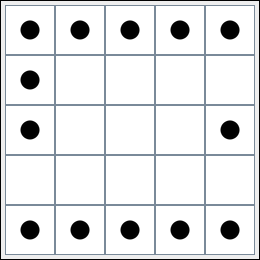
\includegraphics[width=3cm]{Figures/Chromosomes/13a.png} }}
            \qquad
            \subfloat{{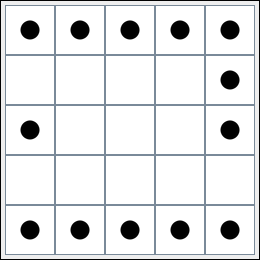
\includegraphics[width=3cm]{Figures/Chromosomes/13b.png} }}
            \qquad
            \subfloat{{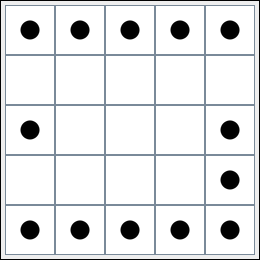
\includegraphics[width=3cm]{Figures/Chromosomes/13c.png} }}
            \qquad
            \subfloat{{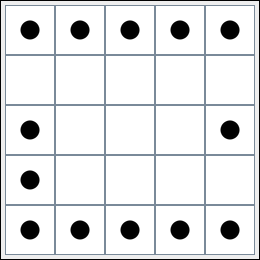
\includegraphics[width=3cm]{Figures/Chromosomes/13d.png} }}
            \qquad
            \subfloat{{
\includegraphics[width=3cm]{Figures/Chromosomes/13e.png} }}
            \qquad
            \subfloat{{
\includegraphics[width=3cm]{Figures/Chromosomes/13f.png} }}
            \qquad
            \subfloat{{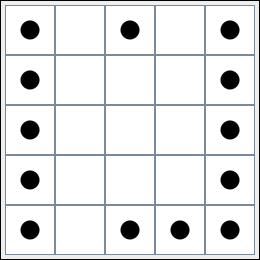
\includegraphics[width=3cm]{Figures/Chromosomes/13g.png} }}
            \qquad
            \subfloat{{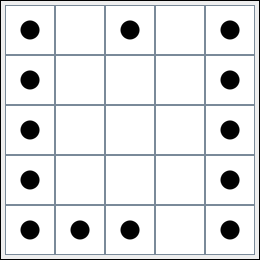
\includegraphics[width=3cm]{Figures/Chromosomes/13h.png} }}
            \caption{Optimal configurations of the small scale problem with 13 wind turbines using exhaustive search method, $obj=0.002110\;kW^{-1}$}
            \label{small13}
        \end{figure}
        
        Figure \ref{small13} shows the optimal configurations of a 1km by 1km wind farm with 13 wind turbines found by exhaustive search. The power output of each wind turbine on the leftmost model in Figure \ref{small13} for different wind directions is shown in Tables \ref{table13a}, \ref{table13b} and \ref{table13c}.
        
        %INSERT TABLE13 HERE
        \singlespacing
        \begin{table}[H]
        	\centering
        	\begin{tabular}{|c|c|c|c|c|c|} \hline
        			& (0 0)		& (0 1)		& (0 2)		& (0 4)		& (1 0)		\\ \hline
        		$0^o$	& 518.4kW	& 518.4kW	& 518.4kW	& 518.4kW	& 293.210kW	\\ \hline
        		$10^o$	& 518.4kW	& 518.4kW	& 518.4kW	& 518.4kW	& 290.474kW	\\ \hline
        		$20^o$	& 518.4kW	& 518.4kW	& 518.4kW	& 518.4kW	& 282.086kW	\\ \hline
        		$30^o$	& 518.4kW	& 518.4kW	& 518.4kW	& 518.4kW	& 347.609kW	\\ \hline
        		$40^o$	& 518.4kW	& 518.4kW	& 518.4kW	& 518.4kW	& 352.743kW	\\ \hline
        		$50^o$	& 518.4kW	& 518.4kW	& 518.4kW	& 518.4kW	& 330.444kW	\\ \hline
        		$60^o$	& 518.4kW	& 518.4kW	& 518.4kW	& 518.4kW	& 324.147kW	\\ \hline
        		$70^o$	& 263.136kW	& 282.086kW	& 397.174kW	& 518.4kW	& 412.245kW	\\ \hline
        		$80^o$	& 270.266kW	& 284.374kW	& 403.702kW	& 518.4kW	& 400.973kW	\\ \hline
        		$90^o$	& 271.221kW	& 281.555kW	& 405.786kW	& 518.4kW	& 444.948kW	\\ \hline
        		$100^o$	& 266.672kW	& 279.437kW	& 368.786kW	& 518.4kW	& 447.713kW	\\ \hline
        		$110^o$	& 258.785kW	& 274.038kW	& 366.773kW	& 518.4kW	& 455.032kW	\\ \hline
        		$120^o$	& 449.876kW	& 429.349kW	& 397.367kW	& 518.4kW	& 454.622kW	\\ \hline
        		$130^o$	& 464.352kW	& 447.565kW	& 387.178kW	& 518.4kW	& 447.030kW	\\ \hline
        		$140^o$	& 463.666kW	& 446.148kW	& 424.308kW	& 518.4kW	& 458.745kW	\\ \hline
        		$150^o$	& 473.721kW	& 451.663kW	& 422.662kW	& 518.4kW	& 467.548kW	\\ \hline
        		$160^o$	& 261.707kW	& 465.930kW	& 454.672kW	& 263.136kW	& 260.131kW	\\ \hline
        		$170^o$	& 263.391kW	& 476.899kW	& 460.065kW	& 265.017kW	& 267.174kW	\\ \hline
        		$180^o$	& 268.237kW	& 430.269kW	& 475.081kW	& 268.237kW	& 270.342kW	\\ \hline
        		$190^o$	& 265.017kW	& 394.135kW	& 460.065kW	& 263.391kW	& 267.174kW	\\ \hline
        		$200^o$	& 263.136kW	& 398.056kW	& 454.672kW	& 261.707kW	& 263.136kW	\\ \hline
        		$210^o$	& 518.4kW	& 317.268kW	& 422.662kW	& 473.721kW	& 518.4kW	\\ \hline
        		$220^o$	& 518.4kW	& 330.444kW	& 424.308kW	& 463.666kW	& 518.4kW	\\ \hline
        		$230^o$	& 518.4kW	& 352.743kW	& 387.178kW	& 464.352kW	& 518.4kW	\\ \hline
        		$240^o$	& 518.4kW	& 347.609kW	& 397.367kW	& 449.876kW	& 518.4kW	\\ \hline
        		$250^o$	& 518.4kW	& 282.086kW	& 252.229kW	& 384.231kW	& 518.4kW	\\ \hline
        		$260^o$	& 518.4kW	& 290.474kW	& 259.714kW	& 373.323kW	& 518.4kW	\\ \hline
        		$270^o$	& 518.4kW	& 293.210kW	& 275.565kW	& 379.355kW	& 518.4kW	\\ \hline
        		$280^o$	& 518.4kW	& 290.474kW	& 272.511kW	& 382.200kW	& 518.4kW	\\ \hline
        		$290^o$	& 518.4kW	& 282.086kW	& 263.136kW	& 397.174kW	& 518.4kW	\\ \hline
        		$300^o$	& 518.4kW	& 518.4kW	& 518.4kW	& 518.4kW	& 518.4kW	\\ \hline
        		$310^o$	& 518.4kW	& 518.4kW	& 518.4kW	& 518.4kW	& 518.4kW	\\ \hline
        		$320^o$	& 518.4kW	& 518.4kW	& 518.4kW	& 518.4kW	& 518.4kW	\\ \hline
        		$330^o$	& 518.4kW	& 518.4kW	& 518.4kW	& 518.4kW	& 518.4kW	\\ \hline
        		$340^o$	& 518.4kW	& 518.4kW	& 518.4kW	& 518.4kW	& 282.086kW	\\ \hline
        		$350^o$	& 518.4kW	& 518.4kW	& 518.4kW	& 518.4kW	& 290.474kW	\\ \hline
        	\end{tabular}
        	\caption{Power output of 13 wind turbines with optimal siting locations resulted from exhaustive search for different wind directions as shown in Figure \ref{small13} (a).}
        	\label{table13a}
        \end{table}
        \begin{table}[H]
        	\centering
        	\begin{tabular}{|c|c|c|c|c|} \hline
        			& (1 4)		& (2 0)		& (2 4)		& (3 0)		\\ \hline
        		$0^o$	& 293.210kW	& 275.565kW	& 275.565kW	& 265.318kW	\\ \hline
        		$10^o$	& 290.474kW	& 259.714kW	& 272.511kW	& 262.830kW	\\ \hline
        		$20^o$	& 282.086kW	& 252.229kW	& 263.136kW	& 256.134kW	\\ \hline
        		$30^o$	& 518.4kW	& 397.367kW	& 518.4kW	& 438.476kW	\\ \hline
        		$40^o$	& 518.4kW	& 396.523kW	& 518.4kW	& 458.745kW	\\ \hline
        		$50^o$	& 518.4kW	& 437.644kW	& 518.4kW	& 447.030kW	\\ \hline
        		$60^o$	& 518.4kW	& 425.807kW	& 518.4kW	& 454.622kW	\\ \hline
        		$70^o$	& 518.4kW	& 463.389kW	& 518.4kW	& 455.032kW	\\ \hline
        		$80^o$	& 518.4kW	& 447.713kW	& 518.4kW	& 447.713kW	\\ \hline
        		$90^o$	& 518.4kW	& 444.948kW	& 518.4kW	& 444.948kW	\\ \hline
        		$100^o$	& 518.4kW	& 447.713kW	& 518.4kW	& 400.973kW	\\ \hline
        		$110^o$	& 518.4kW	& 463.389kW	& 518.4kW	& 412.245kW	\\ \hline
        		$120^o$	& 518.4kW	& 425.807kW	& 518.4kW	& 412.007kW	\\ \hline
        		$130^o$	& 518.4kW	& 437.644kW	& 518.4kW	& 416.779kW	\\ \hline
        		$140^o$	& 518.4kW	& 446.124kW	& 518.4kW	& 518.4kW	\\ \hline
        		$150^o$	& 518.4kW	& 442.995kW	& 518.4kW	& 518.4kW	\\ \hline
        		$160^o$	& 263.136kW	& 263.136kW	& 263.136kW	& 282.086kW	\\ \hline
        		$170^o$	& 267.174kW	& 272.511kW	& 272.511kW	& 290.474kW	\\ \hline
        		$180^o$	& 270.342kW	& 275.565kW	& 275.565kW	& 293.210kW	\\ \hline
        		$190^o$	& 267.174kW	& 272.511kW	& 272.511kW	& 290.474kW	\\ \hline
        		$200^o$	& 260.131kW	& 263.136kW	& 263.136kW	& 282.086kW	\\ \hline
        		$210^o$	& 467.548kW	& 518.4kW	& 442.995kW	& 518.4kW	\\ \hline
        		$220^o$	& 458.745kW	& 518.4kW	& 446.124kW	& 518.4kW	\\ \hline
        		$230^o$	& 447.030kW	& 518.4kW	& 437.644kW	& 518.4kW	\\ \hline
        		$240^o$	& 454.622kW	& 518.4kW	& 425.807kW	& 518.4kW	\\ \hline
        		$250^o$	& 455.032kW	& 518.4kW	& 463.389kW	& 518.4kW	\\ \hline
        		$260^o$	& 447.713kW	& 518.4kW	& 447.713kW	& 518.4kW	\\ \hline
        		$270^o$	& 421.436kW	& 518.4kW	& 444.948kW	& 518.4kW	\\ \hline
        		$280^o$	& 387.940kW	& 518.4kW	& 447.713kW	& 518.4kW	\\ \hline
        		$290^o$	& 398.056kW	& 518.4kW	& 443.215kW	& 518.4kW	\\ \hline
        		$300^o$	& 397.044kW	& 518.4kW	& 414.384kW	& 518.4kW	\\ \hline
        		$310^o$	& 416.779kW	& 518.4kW	& 424.308kW	& 518.4kW	\\ \hline
        		$320^o$	& 518.4kW	& 518.4kW	& 429.738kW	& 518.4kW	\\ \hline
        		$330^o$	& 518.4kW	& 518.4kW	& 442.995kW	& 518.4kW	\\ \hline
        		$340^o$	& 282.086kW	& 263.136kW	& 263.136kW	& 263.136kW	\\ \hline
        		$350^o$	& 290.474kW	& 272.511kW	& 272.511kW	& 267.174kW	\\ \hline
        	\end{tabular}
        	\caption{Power output of 13 wind turbines with optimal siting locations resulted from exhaustive search for different wind directions as shown in Figure \ref{small13} (b).}
        	\label{table13b}
        \end{table}
        \begin{table}[H]
        	\centering
        	\begin{tabular}{|c|c|c|c|c|} \hline
        			& (3 4)		& (4 0)		& (4 2)		& (4 4)		\\ \hline
        		$0^o$	& 270.342kW	& 266.164kW	& 457.869kW	& 268.237kW	\\ \hline
        		$10^o$	& 267.174kW	& 261.560kW	& 460.065kW	& 265.017kW	\\ \hline
        		$20^o$	& 263.136kW	& 259.882kW	& 454.672kW	& 263.136kW	\\ \hline
        		$30^o$	& 518.4kW	& 456.513kW	& 422.662kW	& 518.4kW	\\ \hline
        		$40^o$	& 518.4kW	& 463.666kW	& 424.308kW	& 518.4kW	\\ \hline
        		$50^o$	& 518.4kW	& 464.352kW	& 387.178kW	& 518.4kW	\\ \hline
        		$60^o$	& 518.4kW	& 449.876kW	& 397.367kW	& 518.4kW	\\ \hline
        		$70^o$	& 518.4kW	& 384.231kW	& 366.773kW	& 518.4kW	\\ \hline
        		$80^o$	& 518.4kW	& 386.652kW	& 368.786kW	& 518.4kW	\\ \hline
        		$90^o$	& 518.4kW	& 392.897kW	& 405.786kW	& 518.4kW	\\ \hline
        		$100^o$	& 518.4kW	& 396.867kW	& 403.702kW	& 518.4kW	\\ \hline
        		$110^o$	& 518.4kW	& 397.174kW	& 397.174kW	& 518.4kW	\\ \hline
        		$120^o$	& 518.4kW	& 518.4kW	& 518.4kW	& 518.4kW	\\ \hline
        		$130^o$	& 518.4kW	& 518.4kW	& 518.4kW	& 518.4kW	\\ \hline
        		$140^o$	& 518.4kW	& 518.4kW	& 518.4kW	& 518.4kW	\\ \hline
        		$150^o$	& 518.4kW	& 518.4kW	& 518.4kW	& 518.4kW	\\ \hline
        		$160^o$	& 282.086kW	& 518.4kW	& 518.4kW	& 518.4kW	\\ \hline
        		$170^o$	& 290.474kW	& 518.4kW	& 518.4kW	& 518.4kW	\\ \hline
        		$180^o$	& 293.210kW	& 518.4kW	& 518.4kW	& 518.4kW	\\ \hline
        		$190^o$	& 290.474kW	& 518.4kW	& 518.4kW	& 518.4kW	\\ \hline
        		$200^o$	& 282.086kW	& 518.4kW	& 518.4kW	& 518.4kW	\\ \hline
        		$210^o$	& 518.4kW	& 518.4kW	& 518.4kW	& 518.4kW	\\ \hline
        		$220^o$	& 518.4kW	& 518.4kW	& 518.4kW	& 518.4kW	\\ \hline
        		$230^o$	& 416.779kW	& 518.4kW	& 518.4kW	& 518.4kW	\\ \hline
        		$240^o$	& 412.007kW	& 518.4kW	& 518.4kW	& 518.4kW	\\ \hline
        		$250^o$	& 412.245kW	& 518.4kW	& 397.174kW	& 397.174kW	\\ \hline
        		$260^o$	& 400.973kW	& 518.4kW	& 403.702kW	& 396.867kW	\\ \hline
        		$270^o$	& 444.948kW	& 518.4kW	& 405.786kW	& 392.897kW	\\ \hline
        		$280^o$	& 447.713kW	& 518.4kW	& 368.786kW	& 386.652kW	\\ \hline
        		$290^o$	& 455.032kW	& 518.4kW	& 366.773kW	& 384.231kW	\\ \hline
        		$300^o$	& 443.152kW	& 518.4kW	& 397.367kW	& 449.876kW	\\ \hline
        		$310^o$	& 437.664kW	& 518.4kW	& 387.178kW	& 456.290kW	\\ \hline
        		$320^o$	& 447.565kW	& 518.4kW	& 424.308kW	& 456.290kW	\\ \hline
        		$330^o$	& 453.432kW	& 518.4kW	& 414.384kW	& 464.625kW	\\ \hline
        		$340^o$	& 260.131kW	& 263.136kW	& 443.215kW	& 260.595kW	\\ \hline
        		$350^o$	& 267.174kW	& 265.017kW	& 447.713kW	& 263.391kW	\\ \hline
        	\end{tabular}
        	\caption{Power output of 13 wind turbines with optimal siting locations resulted from exhaustive search for different wind directions as shown in Figure \ref{small13} (c).}
        	\label{table13c}
        \end{table}
        \doublespacing
        
        From Tables \ref{table13a}, \ref{table13b} and \ref{table13c}, the total annual power output of the whole wind farm is $5639.204kW$ which is $83.68\%$ of the theoretical maximum possible power output of a 1km by 1km wind farm with 13 wind turbines, with total cost of
        \begin{align*}
            Cost_{tot}
            &= N\left(\frac{2}{3} + \frac{1}{3}e^{-0.00174N^2}\right) \\
            &= \left(13\right)\left(\frac{2}{3} + \frac{1}{3}e^{-0.00174\left(13^2\right)}\right) \\
            &=11.896
        \end{align*}
        Hence, the fitness of all the chromosomes modelled in Figure \ref{small13} is
        \begin{align*}
            obj
            &=\frac{Cost_{tot}}{P_{tot}} \\
            &=\frac{11.896}{5639.204kW} \\
            &=0.002110kW^{-1}
        \end{align*} 
        
    \textbf{N. 14 Wind Turbines}
        \begin{figure}[H]
            \centering
            \subfloat{{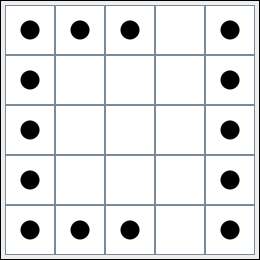
\includegraphics[width=3cm]{Figures/Chromosomes/14a.png} }}
            \qquad
            \subfloat{{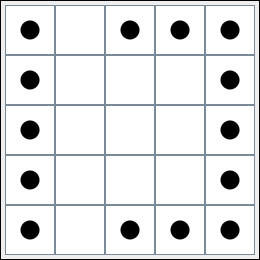
\includegraphics[width=3cm]{Figures/Chromosomes/14b.png} }}
            \qquad
            \subfloat{{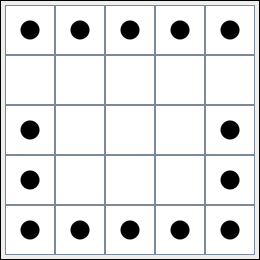
\includegraphics[width=3cm]{Figures/Chromosomes/14c.png} }}
            \qquad
            \subfloat{{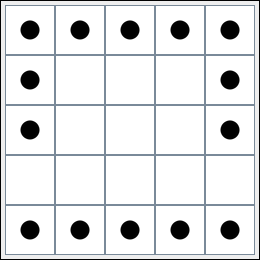
\includegraphics[width=3cm]{Figures/Chromosomes/14d.png} }}
            \caption{Optimal configurations of the small scale problem with 14 wind turbines using exhaustive search method, $obj=0.002113\;kW^{-1}$}
            \label{small14}
        \end{figure}
        
        For 14 wind turbines, the optimal configurations exhausted are shown in Figure \ref{small14}. The power output of each wind turbine on the leftmost model in Figure \ref{small14} for different wind directions is shown in Tables \ref{table14a}, \ref{table14b}, \ref{table14c}.
        
        %INSERT TABLE14 HERE
        \singlespacing
        \begin{table}[H]
        	\centering
        	\begin{tabular}{|c|c|c|c|c|c|} \hline
        			& (0 0)		& (0 1)		& (0 2)		& (0 4)		& (1 0)		\\ \hline
        		$0^o$	& 518.4kW	& 518.4kW	& 518.4kW	& 518.4kW	& 293.210kW	\\ \hline
        		$10^o$	& 518.4kW	& 518.4kW	& 518.4kW	& 518.4kW	& 290.474kW	\\ \hline
        		$20^o$	& 518.4kW	& 518.4kW	& 518.4kW	& 518.4kW	& 282.086kW	\\ \hline
        		$30^o$	& 518.4kW	& 518.4kW	& 518.4kW	& 518.4kW	& 347.609kW	\\ \hline
        		$40^o$	& 518.4kW	& 518.4kW	& 518.4kW	& 518.4kW	& 352.743kW	\\ \hline
        		$50^o$	& 518.4kW	& 518.4kW	& 518.4kW	& 518.4kW	& 330.444kW	\\ \hline
        		$60^o$	& 518.4kW	& 518.4kW	& 518.4kW	& 518.4kW	& 324.147kW	\\ \hline
        		$70^o$	& 263.136kW	& 282.086kW	& 397.174kW	& 518.4kW	& 412.245kW	\\ \hline
        		$80^o$	& 270.266kW	& 284.374kW	& 403.702kW	& 518.4kW	& 400.973kW	\\ \hline
        		$90^o$	& 271.221kW	& 281.555kW	& 405.786kW	& 518.4kW	& 444.948kW	\\ \hline
        		$100^o$	& 266.672kW	& 279.437kW	& 368.786kW	& 518.4kW	& 447.713kW	\\ \hline
        		$110^o$	& 258.785kW	& 274.038kW	& 366.773kW	& 518.4kW	& 455.032kW	\\ \hline
        		$120^o$	& 449.876kW	& 429.349kW	& 397.367kW	& 518.4kW	& 454.622kW	\\ \hline
        		$130^o$	& 464.352kW	& 447.565kW	& 387.178kW	& 518.4kW	& 447.030kW	\\ \hline
        		$140^o$	& 463.666kW	& 446.148kW	& 424.308kW	& 518.4kW	& 458.745kW	\\ \hline
        		$150^o$	& 456.513kW	& 451.663kW	& 422.662kW	& 518.4kW	& 438.476kW	\\ \hline
        		$160^o$	& 259.882kW	& 465.930kW	& 454.672kW	& 263.136kW	& 256.134kW	\\ \hline
        		$170^o$	& 261.560kW	& 458.379kW	& 460.065kW	& 265.017kW	& 262.830kW	\\ \hline
        		$180^o$	& 266.164kW	& 421.436kW	& 457.869kW	& 268.237kW	& 265.318kW	\\ \hline
        		$190^o$	& 265.017kW	& 387.940kW	& 447.713kW	& 263.391kW	& 267.174kW	\\ \hline
        		$200^o$	& 263.136kW	& 398.056kW	& 443.215kW	& 260.595kW	& 263.136kW	\\ \hline
        		$210^o$	& 518.4kW	& 317.268kW	& 414.384kW	& 464.625kW	& 518.4kW	\\ \hline
        		$220^o$	& 518.4kW	& 330.444kW	& 424.308kW	& 456.290kW	& 518.4kW	\\ \hline
        		$230^o$	& 518.4kW	& 352.743kW	& 387.178kW	& 456.290kW	& 518.4kW	\\ \hline
        		$240^o$	& 518.4kW	& 347.609kW	& 397.367kW	& 449.876kW	& 518.4kW	\\ \hline
        		$250^o$	& 518.4kW	& 282.086kW	& 252.229kW	& 384.231kW	& 518.4kW	\\ \hline
        		$260^o$	& 518.4kW	& 290.474kW	& 259.714kW	& 373.323kW	& 518.4kW	\\ \hline
        		$270^o$	& 518.4kW	& 293.210kW	& 275.565kW	& 379.355kW	& 518.4kW	\\ \hline
        		$280^o$	& 518.4kW	& 290.474kW	& 272.511kW	& 382.200kW	& 518.4kW	\\ \hline
        		$290^o$	& 518.4kW	& 282.086kW	& 263.136kW	& 397.174kW	& 518.4kW	\\ \hline
        		$300^o$	& 518.4kW	& 518.4kW	& 518.4kW	& 518.4kW	& 518.4kW	\\ \hline
        		$310^o$	& 518.4kW	& 518.4kW	& 518.4kW	& 518.4kW	& 518.4kW	\\ \hline
        		$320^o$	& 518.4kW	& 518.4kW	& 518.4kW	& 518.4kW	& 518.4kW	\\ \hline
        		$330^o$	& 518.4kW	& 518.4kW	& 518.4kW	& 518.4kW	& 518.4kW	\\ \hline
        		$340^o$	& 518.4kW	& 518.4kW	& 518.4kW	& 518.4kW	& 282.086kW	\\ \hline
        		$350^o$	& 518.4kW	& 518.4kW	& 518.4kW	& 518.4kW	& 290.474kW	\\ \hline
        	\end{tabular}
        	\caption{Power output of 14 wind turbines with optimal siting locations resulted from exhaustive search for different wind directions as shown in Figure \ref{small14} (a).}
        	\label{table14a}
        \end{table}
        \begin{table}[H]
        	\centering
        	\begin{tabular}{|c|c|c|c|c|c|} \hline
        			& (1 4)		& (2 0)		& (2 4)		& (3 0)		& (3 4)		\\ \hline
        		$0^o$	& 293.210kW	& 275.565kW	& 275.565kW	& 265.318kW	& 270.342kW	\\ \hline
        		$10^o$	& 290.474kW	& 259.714kW	& 272.511kW	& 262.830kW	& 267.174kW	\\ \hline
        		$20^o$	& 282.086kW	& 252.229kW	& 263.136kW	& 256.134kW	& 263.136kW	\\ \hline
        		$30^o$	& 518.4kW	& 397.367kW	& 518.4kW	& 438.476kW	& 518.4kW	\\ \hline
        		$40^o$	& 518.4kW	& 396.523kW	& 518.4kW	& 458.745kW	& 518.4kW	\\ \hline
        		$50^o$	& 518.4kW	& 437.644kW	& 518.4kW	& 447.030kW	& 518.4kW	\\ \hline
        		$60^o$	& 518.4kW	& 425.807kW	& 518.4kW	& 454.622kW	& 518.4kW	\\ \hline
        		$70^o$	& 518.4kW	& 463.389kW	& 518.4kW	& 455.032kW	& 518.4kW	\\ \hline
        		$80^o$	& 518.4kW	& 447.713kW	& 518.4kW	& 447.713kW	& 518.4kW	\\ \hline
        		$90^o$	& 518.4kW	& 444.948kW	& 518.4kW	& 444.948kW	& 518.4kW	\\ \hline
        		$100^o$	& 518.4kW	& 447.713kW	& 518.4kW	& 400.973kW	& 518.4kW	\\ \hline
        		$110^o$	& 518.4kW	& 463.389kW	& 518.4kW	& 412.245kW	& 518.4kW	\\ \hline
        		$120^o$	& 518.4kW	& 425.807kW	& 518.4kW	& 324.147kW	& 518.4kW	\\ \hline
        		$130^o$	& 518.4kW	& 437.644kW	& 518.4kW	& 330.444kW	& 518.4kW	\\ \hline
        		$140^o$	& 518.4kW	& 396.523kW	& 518.4kW	& 352.743kW	& 518.4kW	\\ \hline
        		$150^o$	& 518.4kW	& 397.367kW	& 518.4kW	& 347.609kW	& 518.4kW	\\ \hline
        		$160^o$	& 263.136kW	& 252.229kW	& 263.136kW	& 282.086kW	& 282.086kW	\\ \hline
        		$170^o$	& 267.174kW	& 259.714kW	& 272.511kW	& 290.474kW	& 290.474kW	\\ \hline
        		$180^o$	& 270.342kW	& 275.565kW	& 275.565kW	& 293.210kW	& 293.210kW	\\ \hline
        		$190^o$	& 267.174kW	& 272.511kW	& 272.511kW	& 290.474kW	& 290.474kW	\\ \hline
        		$200^o$	& 260.131kW	& 263.136kW	& 263.136kW	& 282.086kW	& 282.086kW	\\ \hline
        		$210^o$	& 453.432kW	& 518.4kW	& 442.995kW	& 518.4kW	& 518.4kW	\\ \hline
        		$220^o$	& 447.565kW	& 518.4kW	& 429.738kW	& 518.4kW	& 518.4kW	\\ \hline
        		$230^o$	& 437.664kW	& 518.4kW	& 424.308kW	& 518.4kW	& 416.779kW	\\ \hline
        		$240^o$	& 443.152kW	& 518.4kW	& 414.384kW	& 518.4kW	& 397.044kW	\\ \hline
        		$250^o$	& 455.032kW	& 518.4kW	& 443.215kW	& 518.4kW	& 398.056kW	\\ \hline
        		$260^o$	& 447.713kW	& 518.4kW	& 447.713kW	& 518.4kW	& 387.940kW	\\ \hline
        		$270^o$	& 421.436kW	& 518.4kW	& 444.948kW	& 518.4kW	& 421.436kW	\\ \hline
        		$280^o$	& 387.940kW	& 518.4kW	& 447.713kW	& 518.4kW	& 447.713kW	\\ \hline
        		$290^o$	& 398.056kW	& 518.4kW	& 443.215kW	& 518.4kW	& 455.032kW	\\ \hline
        		$300^o$	& 397.044kW	& 518.4kW	& 414.384kW	& 518.4kW	& 443.152kW	\\ \hline
        		$310^o$	& 416.779kW	& 518.4kW	& 424.308kW	& 518.4kW	& 437.664kW	\\ \hline
        		$320^o$	& 518.4kW	& 518.4kW	& 429.738kW	& 518.4kW	& 447.565kW	\\ \hline
        		$330^o$	& 518.4kW	& 518.4kW	& 442.995kW	& 518.4kW	& 453.432kW	\\ \hline
        		$340^o$	& 282.086kW	& 263.136kW	& 263.136kW	& 263.136kW	& 260.131kW	\\ \hline
        		$350^o$	& 290.474kW	& 272.511kW	& 272.511kW	& 267.174kW	& 267.174kW	\\ \hline
        	\end{tabular}
        	\caption{Power output of 14 wind turbines with optimal siting locations resulted from exhaustive search for different wind directions as shown in Figure \ref{small14} (b).}
        	\label{table14b}
        \end{table}
        \begin{table}[H]
        	\centering
        	\begin{tabular}{|c|c|c|c|c|} \hline
        			& (4 0)		& (4 1)		& (4 2)		& (4 4)		\\ \hline
        		$0^o$	& 266.164kW	& 421.436kW	& 457.869kW	& 268.237kW	\\ \hline
        		$10^o$	& 261.560kW	& 458.379kW	& 460.065kW	& 265.017kW	\\ \hline
        		$20^o$	& 259.882kW	& 465.930kW	& 454.672kW	& 263.136kW	\\ \hline
        		$30^o$	& 456.513kW	& 451.663kW	& 422.662kW	& 518.4kW	\\ \hline
        		$40^o$	& 463.666kW	& 446.148kW	& 424.308kW	& 518.4kW	\\ \hline
        		$50^o$	& 464.352kW	& 447.565kW	& 387.178kW	& 518.4kW	\\ \hline
        		$60^o$	& 449.876kW	& 429.349kW	& 397.367kW	& 518.4kW	\\ \hline
        		$70^o$	& 258.785kW	& 274.038kW	& 366.773kW	& 518.4kW	\\ \hline
        		$80^o$	& 266.672kW	& 279.437kW	& 368.786kW	& 518.4kW	\\ \hline
        		$90^o$	& 271.221kW	& 281.555kW	& 405.786kW	& 518.4kW	\\ \hline
        		$100^o$	& 270.266kW	& 284.374kW	& 403.702kW	& 518.4kW	\\ \hline
        		$110^o$	& 263.136kW	& 282.086kW	& 397.174kW	& 518.4kW	\\ \hline
        		$120^o$	& 518.4kW	& 518.4kW	& 518.4kW	& 518.4kW	\\ \hline
        		$130^o$ & 518.4kW	& 518.4kW	& 518.4kW	& 518.4kW	\\ \hline
        		$140^o$	& 518.4kW	& 518.4kW	& 518.4kW	& 518.4kW	\\ \hline
        		$150^o$	& 518.4kW	& 518.4kW	& 518.4kW	& 518.4kW	\\ \hline
        		$160^o$ & 518.4kW	& 518.4kW	& 518.4kW	& 518.4kW	\\ \hline
        		$170^o$	& 518.4kW	& 518.4kW	& 518.4kW	& 518.4kW	\\ \hline
        		$180^o$	& 518.4kW	& 518.4kW	& 518.4kW	& 518.4kW	\\ \hline
        		$190^o$	& 518.4kW	& 518.4kW	& 518.4kW	& 518.4kW	\\ \hline
        		$200^o$	& 518.4kW	& 518.4kW	& 518.4kW	& 518.4kW	\\ \hline
        		$210^o$	& 518.4kW	& 518.4kW	& 518.4kW	& 518.4kW	\\ \hline
        		$220^o$	& 518.4kW	& 518.4kW	& 518.4kW	& 518.4kW	\\ \hline
        		$230^o$	& 518.4kW	& 518.4kW	& 518.4kW	& 518.4kW	\\ \hline
        		$240^o$	& 518.4kW	& 518.4kW	& 518.4kW	& 518.4kW	\\ \hline
        		$250^o$	& 518.4kW	& 282.086kW	& 263.136kW	& 397.174kW	\\ \hline
        		$260^o$	& 518.4kW	& 290.474kW	& 272.511kW	& 382.200kW	\\ \hline
        		$270^o$	& 518.4kW	& 293.210kW	& 275.565kW	& 379.355kW	\\ \hline
        		$280^o$	& 518.4kW	& 290.474kW	& 259.714kW	& 373.323kW	\\ \hline
        		$290^o$	& 518.4kW	& 282.086kW	& 252.229kW	& 384.231kW	\\ \hline
        		$300^o$	& 518.4kW	& 347.609kW	& 397.367kW	& 449.876kW	\\ \hline
        		$310^o$	& 518.4kW	& 352.743kW	& 387.178kW	& 456.290kW	\\ \hline
        		$320^o$	& 518.4kW	& 330.444kW	& 424.308kW	& 456.290kW	\\ \hline
        		$330^o$	& 518.4kW	& 317.268kW	& 414.384kW	& 464.625kW	\\ \hline
        		$340^o$	& 263.136kW	& 398.056kW	& 443.215kW	& 260.595kW	\\ \hline
        		$350^o$	& 265.017kW	& 387.940kW	& 447.713kW	& 263.391kW	\\ \hline
        	\end{tabular}
        	\caption{Power output of 14 wind turbines with optimal siting locations resulted from exhaustive search for different wind directions as shown in Figure \ref{small14} (c).}
        	\label{table14c}
        \end{table}
        \doublespacing
        
        From Tables \ref{table14a}, \ref{table14b}, \ref{table14c}, the total annual power output of the whole wind farm is $5988.332kW$ which is $82.51\%$ of the theoretical maximum possible power output of a 1km by 1km wind farm with 14 wind turbines, with total cost of
        \begin{align*}
            Cost_{tot}
            &= N\left(\frac{2}{3} + \frac{1}{3}e^{-0.00174N^2}\right) \\
            &= \left(14\right)\left(\frac{2}{3} + \frac{1}{3}e^{-0.00174\left(14^2\right)}\right) \\
            &=12.651
        \end{align*}
        Hence, the fitness of all the chromosomes modelled in Figure \ref{small14} is
        \begin{align*}
            obj
            &=\frac{Cost_{tot}}{P_{tot}} \\
            &=\frac{12.651}{5988.332kW} \\
            &=0.002113kW^{-1}
        \end{align*}
        
    \textbf{O. 15 Wind Turbines}
        \begin{figure}[H]
            \centering
            \subfloat{{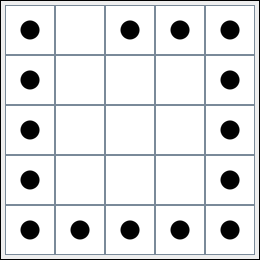
\includegraphics[width=3cm]{Figures/Chromosomes/15a.png} }}
            \qquad
            \subfloat{{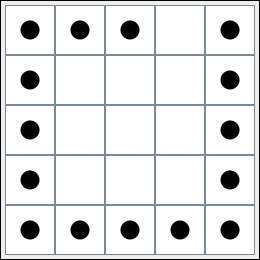
\includegraphics[width=3cm]{Figures/Chromosomes/15b.png} }}
            \qquad
            \subfloat{{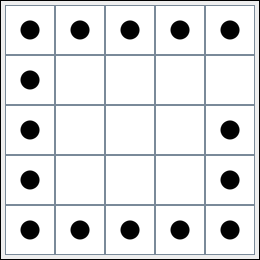
\includegraphics[width=3cm]{Figures/Chromosomes/15c.png} }}
            \qquad
            \subfloat{{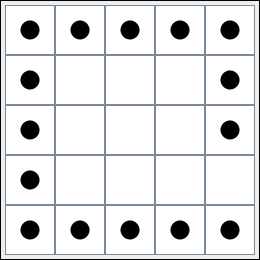
\includegraphics[width=3cm]{Figures/Chromosomes/15d.png} }}
            \qquad
            \subfloat{{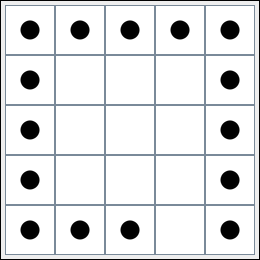
\includegraphics[width=3cm]{Figures/Chromosomes/15e.png} }}
            \qquad
            \subfloat{{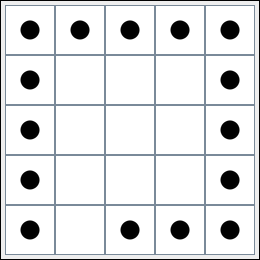
\includegraphics[width=3cm]{Figures/Chromosomes/15f.png} }}
            \qquad
            \subfloat{{\includegraphics[width=3cm]{Figures/Chromosomes/15g.png} }}
            \qquad
            \subfloat{{\includegraphics[width=3cm]{Figures/Chromosomes/15h.png} }}
            \caption{Optimal configurations of the small scale problem with 15 wind turbines using exhaustive search method, $obj=0.002112\;kW^{-1}$}
            \label{small15}
        \end{figure}
        
        The wind farm models from Figure \ref{small15} show the optimal configurations of a 1km by 1km wind farm with 15 wind turbines found by exhaustive search. The power output of each wind turbine on the leftmost model in Figure \ref{small15} for different wind directions is shown in Tables \ref{table15a}, \ref{table15b}, \ref{table15c}.
        
        %INSERT TABLE15 HERE
        \singlespacing
        \begin{table}[H]
        	\centering
        	\begin{tabular}{|c|c|c|c|c|c|} \hline
        			& (0 0)		& (0 2)		& (0 3)		& (0 4)		& (1 0)		\\ \hline
        		$0^o$	& 518.4kW	& 518.4kW	& 518.4kW	& 518.4kW	& 293.210kW	\\ \hline
        		$10^o$	& 518.4kW	& 518.4kW	& 518.4kW	& 518.4kW	& 290.474kW	\\ \hline
        		$20^o$	& 518.4kW	& 518.4kW	& 518.4kW	& 518.4kW	& 282.086kW	\\ \hline
        		$30^o$	& 518.4kW	& 518.4kW	& 518.4kW	& 518.4kW	& 518.4kW	\\ \hline
        		$40^o$	& 518.4kW	& 518.4kW	& 518.4kW	& 518.4kW	& 518.4kW	\\ \hline
        		$50^o$	& 518.4kW	& 518.4kW	& 518.4kW	& 518.4kW	& 416.779kW	\\ \hline
        		$60^o$	& 518.4kW	& 518.4kW	& 518.4kW	& 518.4kW	& 397.044kW	\\ \hline
        		$70^o$	& 397.174kW	& 263.136kW	& 282.086kW	& 518.4kW	& 398.056kW	\\ \hline
        		$80^o$	& 382.200kW	& 272.511kW	& 290.474kW	& 518.4kW	& 387.940kW	\\ \hline
        		$90^o$	& 379.355kW	& 275.565kW	& 293.210kW	& 518.4kW	& 421.436kW	\\ \hline
        		$100^o$	& 373.323kW	& 259.714kW	& 290.474kW	& 518.4kW	& 447.713kW	\\ \hline
        		$110^o$	& 384.231kW	& 252.229kW	& 282.086kW	& 518.4kW	& 455.032kW	\\ \hline
        		$120^o$	& 449.876kW	& 397.367kW	& 347.609kW	& 518.4kW	& 443.152kW	\\ \hline
        		$130^o$	& 456.290kW	& 387.178kW	& 352.743kW	& 518.4kW	& 437.664kW	\\ \hline
        		$140^o$	& 456.290kW	& 424.308kW	& 330.444kW	& 518.4kW	& 447.565kW	\\ \hline
        		$150^o$	& 449.876kW	& 414.384kW	& 317.268kW	& 518.4kW	& 429.349kW	\\ \hline
        		$160^o$	& 258.785kW	& 443.215kW	& 398.056kW	& 263.136kW	& 256.134kW	\\ \hline
        		$170^o$	& 261.560kW	& 447.713kW	& 387.940kW	& 265.017kW	& 262.830kW	\\ \hline
        		$180^o$	& 266.164kW	& 444.948kW	& 421.436kW	& 266.164kW	& 265.318kW	\\ \hline
        		$190^o$	& 265.017kW	& 447.713kW	& 447.713kW	& 261.560kW	& 267.174kW	\\ \hline
        		$200^o$	& 263.136kW	& 443.215kW	& 455.032kW	& 258.785kW	& 263.136kW	\\ \hline
        		$210^o$	& 518.4kW	& 414.384kW	& 443.152kW	& 449.876kW	& 518.4kW	\\ \hline
        		$220^o$	& 518.4kW	& 424.308kW	& 437.664kW	& 456.290kW	& 518.4kW	\\ \hline
        		$230^o$	& 518.4kW	& 387.178kW	& 447.565kW	& 456.290kW	& 518.4kW	\\ \hline
        		$240^o$	& 518.4kW	& 397.367kW	& 429.349kW	& 449.876kW	& 518.4kW	\\ \hline
        		$250^o$	& 518.4kW	& 366.773kW	& 274.038kW	& 258.785kW	& 518.4kW	\\ \hline
        		$260^o$	& 518.4kW	& 368.786kW	& 279.437kW	& 266.672kW	& 518.4kW	\\ \hline
        		$270^o$	& 518.4kW	& 405.786kW	& 281.555kW	& 271.221kW	& 518.4kW	\\ \hline
        		$280^o$	& 518.4kW	& 403.702kW	& 284.374kW	& 270.266kW	& 518.4kW	\\ \hline
        		$290^o$	& 518.4kW	& 397.174kW	& 282.086kW	& 263.136kW	& 518.4kW	\\ \hline
        		$300^o$	& 518.4kW	& 518.4kW	& 518.4kW	& 518.4kW	& 518.4kW	\\ \hline
        		$310^o$	& 518.4kW	& 518.4kW	& 518.4kW	& 518.4kW	& 518.4kW	\\ \hline
        		$320^o$	& 518.4kW	& 518.4kW	& 518.4kW	& 518.4kW	& 518.4kW	\\ \hline
        		$330^o$	& 518.4kW	& 518.4kW	& 518.4kW	& 518.4kW	& 518.4kW	\\ \hline
        		$340^o$	& 518.4kW	& 518.4kW	& 518.4kW	& 518.4kW	& 282.086kW	\\ \hline
        		$350^o$	& 518.4kW	& 518.4kW	& 518.4kW	& 518.4kW	& 290.474kW	\\ \hline
        	\end{tabular}
        	\caption{Power output of 15 wind turbines with optimal siting locations resulted from exhaustive search for different wind directions as shown in Figure \ref{small15} (a).}
        	\label{table15a}
        \end{table}
        \begin{table}[H]
        	\centering
        	\begin{tabular}{|c|c|c|c|c|c|} \hline
        			& (1 4)		& (2 0)		& (2 4)		& (3 0)		& (3 4)		\\ \hline
		$0^o$	& 293.210kW	& 275.565kW	& 275.565kW	& 270.342kW	& 265.318kW	\\ \hline
		$10^o$	& 290.474kW	& 272.511kW	& 272.511kW	& 267.174kW	& 267.174kW	\\ \hline
		$20^o$	& 282.086kW	& 263.136kW	& 263.136kW	& 260.131kW	& 263.136kW	\\ \hline
		$30^o$	& 518.4kW	& 442.995kW	& 518.4kW	& 453.432kW	& 518.4kW	\\ \hline
		$40^o$	& 518.4kW	& 429.738kW	& 518.4kW	& 447.565kW	& 518.4kW	\\ \hline
		$50^o$	& 518.4kW	& 424.308kW	& 518.4kW	& 437.664kW	& 518.4kW	\\ \hline
		$60^o$	& 518.4kW	& 414.384kW	& 518.4kW	& 443.152kW	& 518.4kW	\\ \hline
		$70^o$	& 518.4kW	& 443.215kW	& 518.4kW	& 455.032kW	& 518.4kW	\\ \hline
		$80^o$	& 518.4kW	& 447.713kW	& 518.4kW	& 447.713kW	& 518.4kW	\\ \hline
		$90^o$	& 518.4kW	& 444.948kW	& 518.4kW	& 421.436kW	& 518.4kW	\\ \hline
		$100^o$	& 518.4kW	& 447.713kW	& 518.4kW	& 387.940kW	& 518.4kW	\\ \hline
		$110^o$	& 518.4kW	& 443.215kW	& 518.4kW	& 398.056kW	& 518.4kW	\\ \hline
		$120^o$	& 518.4kW	& 414.384kW	& 518.4kW	& 317.268kW	& 518.4kW	\\ \hline
		$130^o$	& 518.4kW	& 424.308kW	& 518.4kW	& 330.444kW	& 518.4kW	\\ \hline
		$140^o$	& 518.4kW	& 387.178kW	& 518.4kW	& 352.743kW	& 518.4kW	\\ \hline
		$150^o$	& 518.4kW	& 397.367kW	& 518.4kW	& 347.609kW	& 518.4kW	\\ \hline
		$160^o$	& 263.136kW	& 252.229kW	& 263.136kW	& 282.086kW	& 282.086kW	\\ \hline
		$170^o$	& 267.174kW	& 259.714kW	& 272.511kW	& 290.474kW	& 290.474kW	\\ \hline
		$180^o$	& 265.318kW	& 275.565kW	& 275.565kW	& 293.210kW	& 293.210kW	\\ \hline
		$190^o$	& 262.830kW	& 272.511kW	& 259.714kW	& 290.474kW	& 290.474kW	\\ \hline
		$200^o$	& 256.134kW	& 263.136kW	& 252.229kW	& 282.086kW	& 282.086kW	\\ \hline
		$210^o$	& 429.349kW	& 518.4kW	& 397.367kW	& 518.4kW	& 347.609kW	\\ \hline
		$220^o$	& 447.565kW	& 518.4kW	& 387.178kW	& 518.4kW	& 352.743kW	\\ \hline
		$230^o$	& 437.664kW	& 518.4kW	& 424.308kW	& 518.4kW	& 330.444kW	\\ \hline
		$240^o$	& 443.152kW	& 518.4kW	& 414.384kW	& 518.4kW	& 317.268kW	\\ \hline
		$250^o$	& 455.032kW	& 518.4kW	& 443.215kW	& 518.4kW	& 398.056kW	\\ \hline
		$260^o$	& 447.713kW	& 518.4kW	& 447.713kW	& 518.4kW	& 387.940kW	\\ \hline
		$270^o$	& 444.948kW	& 518.4kW	& 444.948kW	& 518.4kW	& 421.436kW	\\ \hline
		$280^o$	& 400.973kW	& 518.4kW	& 447.713kW	& 518.4kW	& 447.713kW	\\ \hline
		$290^o$	& 412.245kW	& 518.4kW	& 463.389kW	& 518.4kW	& 455.032kW	\\ \hline
		$300^o$	& 324.147kW	& 518.4kW	& 425.807kW	& 518.4kW	& 454.622kW	\\ \hline
		$310^o$	& 330.444kW	& 518.4kW	& 437.644kW	& 518.4kW	& 447.030kW	\\ \hline
		$320^o$	& 352.743kW	& 518.4kW	& 396.523kW	& 518.4kW	& 458.745kW	\\ \hline
		$330^o$	& 347.609kW	& 518.4kW	& 397.367kW	& 518.4kW	& 438.476kW	\\ \hline
		$340^o$	& 282.086kW	& 263.136kW	& 252.229kW	& 263.136kW	& 256.134kW	\\ \hline
		$350^o$	& 290.474kW	& 272.511kW	& 259.714kW	& 267.174kW	& 262.830kW	\\ \hline
        	\end{tabular}
        	\caption{Power output of 15 wind turbines with optimal siting locations resulted from exhaustive search for different wind directions as shown in Figure \ref{small15} (b).}
        	\label{table15b}
        \end{table}
        \begin{table}[H]
        	\centering
        	\begin{tabular}{|c|c|c|c|c|c|} \hline
        			& (4 0)		& (4 1)		& (4 2)		& (4 3)		& (4 4)		\\ \hline
		$0^o$	& 268.237kW	& 430.269kW	& 457.869kW	& 421.436kW	& 266.164kW	\\ \hline
		$10^o$	& 263.391kW	& 462.133kW	& 447.713kW	& 387.940kW	& 265.017kW	\\ \hline
		$20^o$	& 260.595kW	& 455.032kW	& 443.215kW	& 398.056kW	& 263.136kW	\\ \hline
		$30^o$	& 464.625kW	& 443.152kW	& 414.384kW	& 317.268kW	& 518.4kW	\\ \hline
		$40^o$	& 456.290kW	& 437.664kW	& 424.308kW	& 330.444kW	& 518.4kW	\\ \hline
		$50^o$	& 456.290kW	& 447.565kW	& 387.178kW	& 352.743kW	& 518.4kW	\\ \hline
		$60^o$	& 449.876kW	& 429.349kW	& 397.367kW	& 347.609kW	& 518.4kW	\\ \hline
		$70^o$	& 258.785kW	& 256.134kW	& 252.229kW	& 282.086kW	& 518.4kW	\\ \hline
		$80^o$	& 261.560kW	& 262.830kW	& 259.714kW	& 290.474kW	& 518.4kW	\\ \hline
		$90^o$	& 266.164kW	& 265.318kW	& 275.565kW	& 293.210kW	& 518.4kW	\\ \hline
		$100^o$	& 265.017kW	& 267.174kW	& 272.511kW	& 290.474kW	& 518.4kW	\\ \hline
		$110^o$	& 263.136kW	& 263.136kW	& 263.136kW	& 282.086kW	& 518.4kW	\\ \hline
		$120^o$	& 518.4kW	& 518.4kW	& 518.4kW	& 518.4kW	& 518.4kW	\\ \hline
		$130^o$	& 518.4kW	& 518.4kW	& 518.4kW	& 518.4kW	& 518.4kW	\\ \hline
		$140^o$	& 518.4kW	& 518.4kW	& 518.4kW	& 518.4kW	& 518.4kW	\\ \hline
		$150^o$	& 518.4kW	& 518.4kW	& 518.4kW	& 518.4kW	& 518.4kW	\\ \hline
		$160^o$	& 518.4kW	& 518.4kW	& 518.4kW	& 518.4kW	& 518.4kW	\\ \hline
		$170^o$	& 518.4kW	& 518.4kW	& 518.4kW	& 518.4kW	& 518.4kW	\\ \hline
		$180^o$	& 518.4kW	& 518.4kW	& 518.4kW	& 518.4kW	& 518.4kW	\\ \hline
		$190^o$	& 518.4kW	& 518.4kW	& 518.4kW	& 518.4kW	& 518.4kW	\\ \hline
		$200^o$	& 518.4kW	& 518.4kW	& 518.4kW	& 518.4kW	& 518.4kW	\\ \hline
		$210^o$	& 518.4kW	& 518.4kW	& 518.4kW	& 518.4kW	& 518.4kW	\\ \hline
		$220^o$	& 518.4kW	& 518.4kW	& 518.4kW	& 518.4kW	& 518.4kW	\\ \hline
		$230^o$	& 518.4kW	& 518.4kW	& 518.4kW	& 518.4kW	& 518.4kW	\\ \hline
		$240^o$	& 518.4kW	& 518.4kW	& 518.4kW	& 518.4kW	& 518.4kW	\\ \hline
		$250^o$	& 518.4kW	& 282.086kW	& 263.136kW	& 263.136kW	& 263.136kW	\\ \hline
		$260^o$	& 518.4kW	& 290.474kW	& 272.511kW	& 267.174kW	& 265.017kW	\\ \hline
		$270^o$	& 518.4kW	& 293.210kW	& 275.565kW	& 265.318kW	& 266.164kW	\\ \hline
		$280^o$	& 518.4kW	& 290.474kW	& 259.714kW	& 262.830kW	& 261.560kW	\\ \hline
		$290^o$	& 518.4kW	& 282.086kW	& 252.229kW	& 256.134kW	& 258.785kW	\\ \hline
		$300^o$	& 518.4kW	& 347.609kW	& 397.367kW	& 429.349kW	& 449.876kW	\\ \hline
		$310^o$	& 518.4kW	& 352.743kW	& 387.178kW	& 447.565kW	& 464.352kW	\\ \hline
		$320^o$	& 518.4kW	& 330.444kW	& 424.308kW	& 446.148kW	& 463.666kW	\\ \hline
		$330^o$	& 518.4kW	& 317.268kW	& 422.662kW	& 451.663kW	& 456.513kW	\\ \hline
		$340^o$	& 263.136kW	& 398.056kW	& 454.672kW	& 465.930kW	& 259.882kW	\\ \hline
		$350^o$	& 265.017kW	& 394.135kW	& 460.065kW	& 458.379kW	& 261.560kW	\\ \hline
        	\end{tabular}
        	\caption{Power output of 15 wind turbines with optimal siting locations resulted from exhaustive search for different wind directions as shown in Figure \ref{small15} (b).}
        	\label{table15c}
        \end{table}
        \doublespacing
        
        From Tables \ref{table15a}, \ref{table15b}, \ref{table15c}, the total annual power output of the whole wind farm is $6335.066kW$ which is $81.47\%$ of the theoretical maximum possible power output of a 1km by 1km wind farm with 15 wind turbines, with total cost of
        \begin{align*}
            Cost_{tot}
            &= N\left(\frac{2}{3} + \frac{1}{3}e^{-0.00174N^2}\right) \\
            &= \left(15\right)\left(\frac{2}{3} + \frac{1}{3}e^{-0.00174\left(15^2\right)}\right) \\
            &=13.380
        \end{align*}
        Hence, the fitness of all the chromosomes modelled in Figure \ref{small15} is
        \begin{align*}
            obj
            &=\frac{Cost_{tot}}{P_{tot}} \\
            &=\frac{13.380}{6335.066kW} \\
            &=0.002112kW^{-1}
        \end{align*}
        
    \textbf{P. 16 Wind Turbines}
        \begin{figure}[H]
            \centering
            \includegraphics[width=3cm]{Figures/Chromosomes/16.png}
            \caption{Optimal configuration of the small scale problem with 16 wind turbines using exhaustive search method, $obj=0.002108\;kW^{-1}$}
            \label{small16}
        \end{figure}
        
        For 16 turbines on a 1km by 1km wind farm, it is trivial that the optimal solution is that the wind turbines are located at the edges of the wind farm as shown in Figure \ref{16}. The power output of each wind turbine on the leftmost model in Figure \ref{small16} for different wind directions is shown in Tables \ref{table16a}, \ref{table16b}, \ref{table16c}.
        
        %INSERT TABLE16 HERE
        \singlespacing
        \begin{table}[H]
        	\centering
        	\begin{tabular}{|c|c|c|c|c|c|c|} \hline
        			& (0 0)		& (0 1)		& (0 2)		& (0 3)		& (0 4)		& (1 0)		\\ \hline
		$0^o$	& 518.4kW	& 518.4kW	& 518.4kW	& 518.4kW	& 518.4kW	& 293.210kW	\\ \hline
		$10^o$	& 518.4kW	& 518.4kW	& 518.4kW	& 518.4kW	& 518.4kW	& 290.474kW	\\ \hline
		$20^o$	& 518.4kW	& 518.4kW	& 518.4kW	& 518.4kW	& 518.4kW	& 282.086kW	\\ \hline
		$30^o$	& 518.4kW	& 518.4kW	& 518.4kW	& 518.4kW	& 518.4kW	& 347.609kW	\\ \hline
		$40^o$	& 518.4kW	& 518.4kW	& 518.4kW	& 518.4kW	& 518.4kW	& 352.743kW	\\ \hline
		$50^o$	& 518.4kW	& 518.4kW	& 518.4kW	& 518.4kW	& 518.4kW	& 330.444kW	\\ \hline
		$60^o$	& 518.4kW	& 518.4kW	& 518.4kW	& 518.4kW	& 518.4kW	& 317.268kW	\\ \hline
		$70^o$	& 263.136kW	& 263.136kW	& 263.136kW	& 282.086kW	& 518.4kW	& 398.056kW	\\ \hline
		$80^o$	& 265.017kW	& 267.174kW	& 272.511kW	& 290.474kW	& 518.4kW	& 387.940kW	\\ \hline
		$90^o$	& 266.164kW	& 265.318kW	& 275.565kW	& 293.210kW	& 518.4kW	& 421.436kW	\\ \hline
		$100^o$	& 261.560kW	& 262.830kW	& 259.714kW	& 290.474kW	& 518.4kW	& 447.713kW	\\ \hline
		$110^o$	& 258.785kW	& 256.134kW	& 252.229kW	& 282.086kW	& 518.4kW	& 455.032kW	\\ \hline
		$120^o$	& 449.876kW	& 429.349kW	& 397.367kW	& 347.609kW	& 518.4kW	& 443.152kW	\\ \hline
		$130^o$	& 456.290kW	& 447.565kW	& 387.178kW	& 352.743kW	& 518.4kW	& 437.664kW	\\ \hline
		$140^o$	& 456.290kW	& 437.664kW	& 424.308kW	& 330.444kW	& 518.4kW	& 447.565kW	\\ \hline
		$150^o$	& 449.876kW	& 443.152kW	& 414.384kW	& 317.268kW	& 518.4kW	& 429.349kW	\\ \hline
		$160^o$	& 258.785kW	& 455.032kW	& 443.215kW	& 398.056kW	& 263.136kW	& 256.134kW	\\ \hline
		$170^o$	& 261.560kW	& 447.713kW	& 447.713kW	& 387.940kW	& 265.017kW	& 262.830kW	\\ \hline
		$180^o$	& 266.164kW	& 421.436kW	& 444.948kW	& 421.436kW	& 266.164kW	& 265.318kW	\\ \hline
		$190^o$	& 265.017kW	& 387.940kW	& 447.713kW	& 447.713kW	& 261.560kW	& 267.174kW	\\ \hline
		$200^o$	& 263.136kW	& 398.056kW	& 443.215kW	& 455.032kW	& 258.785kW	& 263.136kW	\\ \hline
		$210^o$	& 518.4kW	& 317.268kW	& 414.384kW	& 443.152kW	& 449.876kW	& 518.4kW	\\ \hline
		$220^o$	& 518.4kW	& 330.444kW	& 424.308kW	& 437.664kW	& 456.290kW	& 518.4kW	\\ \hline
		$230^o$	& 518.4kW	& 352.743kW	& 387.178kW	& 447.565kW	& 456.290kW	& 518.4kW	\\ \hline
		$240^o$	& 518.4kW	& 347.609kW	& 397.367kW	& 429.349kW	& 449.876kW	& 518.4kW	\\ \hline
		$250^o$	& 518.4kW	& 282.086kW	& 252.229kW	& 256.134kW	& 258.785kW	& 518.4kW	\\ \hline
		$260^o$	& 518.4kW	& 290.474kW	& 259.714kW	& 262.830kW	& 261.560kW	& 518.4kW	\\ \hline
		$270^o$	& 518.4kW	& 293.210kW	& 275.565kW	& 265.318kW	& 266.164kW	& 518.4kW	\\ \hline
		$280^o$	& 518.4kW	& 290.474kW	& 272.511kW	& 267.174kW	& 265.017kW	& 518.4kW	\\ \hline
		$290^o$	& 518.4kW	& 282.086kW	& 263.136kW	& 263.136kW	& 263.136kW	& 518.4kW	\\ \hline
		$300^o$	& 518.4kW	& 518.4kW	& 518.4kW	& 518.4kW	& 518.4kW	& 518.4kW	\\ \hline
		$310^o$	& 518.4kW	& 518.4kW	& 518.4kW	& 518.4kW	& 518.4kW	& 518.4kW	\\ \hline
		$320^o$	& 518.4kW	& 518.4kW	& 518.4kW	& 518.4kW	& 518.4kW	& 518.4kW	\\ \hline
		$330^o$	& 518.4kW	& 518.4kW	& 518.4kW	& 518.4kW	& 518.4kW	& 518.4kW	\\ \hline
		$340^o$	& 518.4kW	& 518.4kW	& 518.4kW	& 518.4kW	& 518.4kW	& 282.086kW	\\ \hline
		$350^o$	& 518.4kW	& 518.4kW	& 518.4kW	& 518.4kW	& 518.4kW	& 290.474kW	\\ \hline
        	\end{tabular}
        	\caption{Power output of 16 wind turbines with optimal siting locations resulted from exhaustive search for different wind directions as shown in Figure \ref{small16} (a).}
        	\label{table16a}
        \end{table}
        \begin{table}[H]
        	\centering
        	\begin{tabular}{|c|c|c|c|c|c|} \hline
        			& (1 4)		& (2 0)		& (2 4)		& (3 0)		& (3 4)		\\ \hline
		$0^o$	& 293.210kW	& 275.565kW	& 275.565kW	& 265.318kW	& 265.318kW	\\ \hline
		$10^o$	& 290.474kW	& 259.714kW	& 272.511kW	& 262.830kW	& 267.174kW	\\ \hline
		$20^o$	& 282.086kW	& 252.229kW	& 263.136kW	& 256.134kW	& 263.136kW	\\ \hline
		$30^o$	& 518.4kW	& 397.367kW	& 518.4kW	& 429.349kW	& 518.4kW	\\ \hline
		$40^o$	& 518.4kW	& 387.178kW	& 518.4kW	& 447.565kW	& 518.4kW	\\ \hline
		$50^o$	& 518.4kW	& 424.308kW	& 518.4kW	& 437.664kW	& 518.4kW	\\ \hline
		$60^o$	& 518.4kW	& 414.384kW	& 518.4kW	& 443.152kW	& 518.4kW	\\ \hline
		$70^o$	& 518.4kW	& 443.215kW	& 518.4kW	& 455.032kW	& 518.4kW	\\ \hline
		$80^o$	& 518.4kW	& 447.713kW	& 518.4kW	& 447.713kW	& 518.4kW	\\ \hline
		$90^o$	& 518.4kW	& 444.948kW	& 518.4kW	& 421.436kW	& 518.4kW	\\ \hline
		$100^o$	& 518.4kW	& 447.713kW	& 518.4kW	& 387.940kW	& 518.4kW	\\ \hline
		$110^o$	& 518.4kW	& 443.215kW	& 518.4kW	& 398.056kW	& 518.4kW	\\ \hline
		$120^o$	& 518.4kW	& 414.384kW	& 518.4kW	& 317.268kW	& 518.4kW	\\ \hline
		$130^o$	& 518.4kW	& 424.308kW	& 518.4kW	& 330.444kW	& 518.4kW	\\ \hline
		$140^o$	& 518.4kW	& 387.178kW	& 518.4kW	& 352.743kW	& 518.4kW	\\ \hline
		$150^o$	& 518.4kW	& 397.367kW	& 518.4kW	& 347.609kW	& 518.4kW	\\ \hline
		$160^o$	& 263.136kW	& 252.229kW	& 263.136kW	& 282.086kW	& 282.086kW	\\ \hline
		$170^o$	& 267.174kW	& 259.714kW	& 272.511kW	& 290.474kW	& 290.474kW	\\ \hline
		$180^o$	& 265.318kW	& 275.565kW	& 275.565kW	& 293.210kW	& 293.210kW	\\ \hline
		$190^o$	& 262.830kW	& 272.511kW	& 259.714kW	& 290.474kW	& 290.474kW	\\ \hline
		$200^o$	& 256.134kW	& 263.136kW	& 252.229kW	& 282.086kW	& 282.086kW	\\ \hline
		$210^o$	& 429.349kW	& 518.4kW	& 397.367kW	& 518.4kW	& 347.609kW	\\ \hline
		$220^o$	& 447.565kW	& 518.4kW	& 387.178kW	& 518.4kW	& 352.743kW	\\ \hline
		$230^o$	& 437.664kW	& 518.4kW	& 424.308kW	& 518.4kW	& 330.444kW	\\ \hline
		$240^o$	& 443.152kW	& 518.4kW	& 414.384kW	& 518.4kW	& 317.268kW	\\ \hline
		$250^o$	& 455.032kW	& 518.4kW	& 443.215kW	& 518.4kW	& 398.056kW	\\ \hline
		$260^o$	& 447.713kW	& 518.4kW	& 447.713kW	& 518.4kW	& 387.940kW	\\ \hline
		$270^o$	& 421.436kW	& 518.4kW	& 444.948kW	& 518.4kW	& 421.436kW	\\ \hline
		$280^o$	& 387.940kW	& 518.4kW	& 447.713kW	& 518.4kW	& 447.713kW	\\ \hline
		$290^o$	& 398.056kW	& 518.4kW	& 443.215kW	& 518.4kW	& 455.032kW	\\ \hline
		$300^o$	& 317.268kW	& 518.4kW	& 414.384kW	& 518.4kW	& 443.152kW	\\ \hline
		$310^o$	& 330.444kW	& 518.4kW	& 424.308kW	& 518.4kW	& 437.664kW	\\ \hline
		$320^o$	& 352.743kW	& 518.4kW	& 387.178kW	& 518.4kW	& 447.565kW	\\ \hline
		$330^o$	& 347.609kW	& 518.4kW	& 397.367kW	& 518.4kW	& 429.349kW	\\ \hline
		$340^o$	& 282.086kW	& 263.136kW	& 252.229kW	& 263.136kW	& 256.134kW	\\ \hline
		$350^o$	& 290.474kW	& 272.511kW	& 259.714kW	& 267.174kW	& 262.830kW	\\ \hline
        	\end{tabular}
        	\caption{Power output of 16 wind turbines with optimal siting locations resulted from exhaustive search for different wind directions as shown in Figure \ref{small16} (b).}
        	\label{table16b}
        \end{table}
        \begin{table}[H]
        	\centering
        	\begin{tabular}{|c|c|c|c|c|c|} \hline
        			& (4 0)		& (4 1)		& (4 2)		& (4 3)		& (4 4)		\\ \hline
		$0^o$	& 266.164kW	& 421.436kW	& 444.948kW	& 421.436kW	& 266.164kW	\\ \hline
		$10^o$	& 261.560kW	& 447.713kW	& 447.713kW	& 387.940kW	& 265.017kW	\\ \hline
		$20^o$	& 258.785kW	& 455.032kW	& 443.215kW	& 398.056kW	& 263.136kW	\\ \hline
		$30^o$	& 449.876kW	& 443.152kW	& 414.384kW	& 317.268kW	& 518.4kW	\\ \hline
		$40^o$	& 456.290kW	& 437.664kW	& 424.308kW	& 330.444kW	& 518.4kW	\\ \hline
		$50^o$	& 456.290kW	& 447.565kW	& 387.178kW	& 352.743kW	& 518.4kW	\\ \hline
		$60^o$	& 449.876kW	& 429.349kW	& 397.367kW	& 347.609kW	& 518.4kW	\\ \hline
		$70^o$	& 258.785kW	& 256.134kW	& 252.229kW	& 282.086kW	& 518.4kW	\\ \hline
		$80^o$	& 261.560kW	& 262.830kW	& 259.714kW	& 290.474kW	& 518.4kW	\\ \hline
		$90^o$	& 266.164kW	& 265.318kW	& 275.565kW	& 293.210kW	& 518.4kW	\\ \hline
		$100^o$	& 265.017kW	& 267.174kW	& 272.511kW	& 290.474kW	& 518.4kW	\\ \hline
		$110^o$	& 263.136kW	& 263.136kW	& 263.136kW	& 282.086kW	& 518.4kW	\\ \hline
		$120^o$	& 518.4kW	& 518.4kW	& 518.4kW	& 518.4kW	& 518.4kW	\\ \hline
		$130^o$	& 518.4kW	& 518.4kW	& 518.4kW	& 518.4kW	& 518.4kW	\\ \hline
		$140^o$	& 518.4kW	& 518.4kW	& 518.4kW	& 518.4kW	& 518.4kW	\\ \hline
		$150^o$	& 518.4kW	& 518.4kW	& 518.4kW	& 518.4kW	& 518.4kW	\\ \hline
		$160^o$	& 518.4kW	& 518.4kW	& 518.4kW	& 518.4kW	& 518.4kW	\\ \hline
		$170^o$	& 518.4kW	& 518.4kW	& 518.4kW	& 518.4kW	& 518.4kW	\\ \hline
		$180^o$	& 518.4kW	& 518.4kW	& 518.4kW	& 518.4kW	& 518.4kW	\\ \hline
		$190^o$	& 518.4kW	& 518.4kW	& 518.4kW	& 518.4kW	& 518.4kW	\\ \hline
		$200^o$	& 518.4kW	& 518.4kW	& 518.4kW	& 518.4kW	& 518.4kW	\\ \hline
		$210^o$	& 518.4kW	& 518.4kW	& 518.4kW	& 518.4kW	& 518.4kW	\\ \hline
		$220^o$	& 518.4kW	& 518.4kW	& 518.4kW	& 518.4kW	& 518.4kW	\\ \hline
		$230^o$	& 518.4kW	& 518.4kW	& 518.4kW	& 518.4kW	& 518.4kW	\\ \hline
		$240^o$	& 518.4kW	& 518.4kW	& 518.4kW	& 518.4kW	& 518.4kW	\\ \hline
		$250^o$	& 518.4kW	& 282.086kW	& 263.136kW	& 263.136kW	& 263.136kW	\\ \hline
		$260^o$	& 518.4kW	& 290.474kW	& 272.511kW	& 267.174kW	& 265.017kW	\\ \hline
		$270^o$	& 518.4kW	& 293.210kW	& 275.565kW	& 265.318kW	& 266.164kW	\\ \hline
		$280^o$	& 518.4kW	& 290.474kW	& 259.714kW	& 262.830kW	& 261.560kW	\\ \hline
		$290^o$	& 518.4kW	& 282.086kW	& 252.229kW	& 256.134kW	& 258.785kW	\\ \hline
		$300^o$	& 518.4kW	& 347.609kW	& 397.367kW	& 429.349kW	& 449.876kW	\\ \hline
		$310^o$	& 518.4kW	& 352.743kW	& 387.178kW	& 447.565kW	& 456.290kW	\\ \hline
		$320^o$	& 518.4kW	& 330.444kW	& 424.308kW	& 437.664kW	& 456.290kW	\\ \hline
		$330^o$	& 518.4kW	& 317.268kW	& 414.384kW	& 443.152kW	& 449.876kW	\\ \hline
		$340^o$	& 263.136kW	& 398.056kW	& 443.215kW	& 455.032kW	& 258.785kW	\\ \hline
		$350^o$	& 265.017kW	& 387.940kW	& 447.713kW	& 447.713kW	& 261.560kW	\\ \hline
        	\end{tabular}
        	\caption{Power output of 16 wind turbines with optimal siting locations resulted from exhaustive search for different wind directions as shown in Figure \ref{small16} (c).}
        	\label{table16c}
        \end{table}
        \doublespacing
        
        From Tables \ref{table16a}, \ref{table16b}, \ref{table16c}, the total annual power output of the whole wind farm is $6680.164kW$ which is $80.54\%$ of the theoretical maximum possible power output of a 1km by 1km wind farm with 16 wind turbines, with total cost of
        \begin{align*}
            Cost_{tot}
            &= N\left(\frac{2}{3} + \frac{1}{3}e^{-0.00174N^2}\right) \\
            &= \left(16\right)\left(\frac{2}{3} + \frac{1}{3}e^{-0.00174\left(16^2\right)}\right) \\
            &=14.083
        \end{align*}
        Hence, the fitness of the chromosome modelled in Figure \ref{small16} is
        \begin{align*}
            obj
            &=\frac{Cost_{tot}}{P_{tot}} \\
            &=\frac{14.083}{6680.164kW} \\
            &=0.002108kW^{-1}
        \end{align*}
        
    \textbf{Q. 17 Wind Turbines}
        \begin{figure}[H]
            \centering
            \includegraphics[width=3cm]{Figures/Chromosomes/17.png}
            \caption{Optimal configuration of the small scale problem with 17 wind turbines using exhaustive search method, $obj=0.002117\;kW^{-1}$}
            \label{small17}
        \end{figure}
        
        The optimal solution for 17 wind turbines found by exhaustive search is the same as with the optimal solution for 16 wind turbines with an additional wind turbine at the center of the wind farm as shown in Figure \ref{small17}. The power output of each wind turbine on the leftmost model in Figure \ref{small17} for different wind directions is shown in Tables \ref{table17a}, \ref{table17b}, \ref{table17c}.
        
        %INSERT TABLE17 HERE
        \singlespacing
        \begin{table}[H]
        	\centering
        	\begin{tabular}{|c|c|c|c|c|c|c|} \hline
        			& (0 0)		& (0 1)		& (0 2)		& (0 3)		& (0 4)		& (1 0)		\\ \hline
		$0^o$	& 518.4kW	& 518.4kW	& 518.4kW	& 518.4kW	& 518.4kW	& 293.210kW	\\ \hline
		$10^o$	& 518.4kW	& 518.4kW	& 518.4kW	& 518.4kW	& 518.4kW	& 290.474kW	\\ \hline
		$20^o$	& 518.4kW	& 518.4kW	& 518.4kW	& 518.4kW	& 518.4kW	& 282.086kW	\\ \hline
		$30^o$	& 518.4kW	& 518.4kW	& 518.4kW	& 518.4kW	& 518.4kW	& 347.609kW	\\ \hline
		$40^o$	& 518.4kW	& 518.4kW	& 518.4kW	& 518.4kW	& 518.4kW	& 352.743kW	\\ \hline
		$50^o$	& 518.4kW	& 518.4kW	& 518.4kW	& 518.4kW	& 518.4kW	& 330.444kW	\\ \hline
		$60^o$	& 518.4kW	& 518.4kW	& 518.4kW	& 518.4kW	& 518.4kW	& 317.268kW	\\ \hline
		$70^o$	& 263.136kW	& 263.136kW	& 263.136kW	& 282.086kW	& 518.4kW	& 398.056kW	\\ \hline
		$80^o$	& 265.017kW	& 267.174kW	& 272.511kW	& 290.474kW	& 518.4kW	& 387.940kW	\\ \hline
		$90^o$	& 266.164kW	& 265.318kW	& 275.565kW	& 293.210kW	& 518.4kW	& 421.436kW	\\ \hline
		$100^o$	& 261.560kW	& 262.830kW	& 259.714kW	& 290.474kW	& 518.4kW	& 395.853kW	\\ \hline
		$110^o$	& 258.785kW	& 256.134kW	& 252.229kW	& 282.086kW	& 518.4kW	& 403.210kW	\\ \hline
		$120^o$	& 418.565kW	& 429.349kW	& 397.367kW	& 347.609kW	& 518.4kW	& 397.455kW	\\ \hline
		$130^o$	& 424.871kW	& 447.565kW	& 387.178kW	& 352.743kW	& 518.4kW	& 391.865kW	\\ \hline
		$140^o$	& 424.871kW	& 391.865kW	& 424.308kW	& 330.444kW	& 518.4kW	& 447.565kW	\\ \hline
		$150^o$	& 418.565kW	& 397.455kW	& 414.384kW	& 317.268kW	& 518.4kW	& 429.349kW	\\ \hline
		$160^o$	& 258.785kW	& 403.210kW	& 379.127kW	& 398.056kW	& 263.136kW	& 256.134kW	\\ \hline
		$170^o$	& 261.560kW	& 395.853kW	& 386.652kW	& 387.940kW	& 265.017kW	& 262.830kW	\\ \hline
		$180^o$	& 266.164kW	& 421.436kW	& 387.058kW	& 421.436kW	& 266.164kW	& 265.318kW	\\ \hline
		$190^o$	& 265.017kW	& 387.940kW	& 386.652kW	& 395.853kW	& 261.560kW	& 267.174kW	\\ \hline
		$200^o$	& 263.136kW	& 398.056kW	& 379.127kW	& 403.210kW	& 258.785kW	& 263.136kW	\\ \hline
		$210^o$	& 518.4kW	& 317.268kW	& 414.384kW	& 397.455kW	& 418.565kW	& 518.4kW	\\ \hline
		$220^o$	& 518.4kW	& 330.444kW	& 424.308kW	& 391.865kW	& 424.871kW	& 518.4kW	\\ \hline
		$230^o$	& 518.4kW	& 352.743kW	& 387.178kW	& 447.565kW	& 424.871kW	& 518.4kW	\\ \hline
		$240^o$	& 518.4kW	& 347.609kW	& 397.367kW	& 429.349kW	& 418.565kW	& 518.4kW	\\ \hline
		$250^o$	& 518.4kW	& 282.086kW	& 252.229kW	& 256.134kW	& 258.785kW	& 518.4kW	\\ \hline
		$260^o$	& 518.4kW	& 290.474kW	& 259.714kW	& 262.830kW	& 261.560kW	& 518.4kW	\\ \hline
		$270^o$	& 518.4kW	& 293.210kW	& 275.565kW	& 265.318kW	& 266.164kW	& 518.4kW	\\ \hline
		$280^o$	& 518.4kW	& 290.474kW	& 272.511kW	& 267.174kW	& 265.017kW	& 518.4kW	\\ \hline
		$290^o$	& 518.4kW	& 282.086kW	& 263.136kW	& 263.136kW	& 263.136kW	& 518.4kW	\\ \hline
		$300^o$	& 518.4kW	& 518.4kW	& 518.4kW	& 518.4kW	& 518.4kW	& 518.4kW	\\ \hline
		$310^o$	& 518.4kW	& 518.4kW	& 518.4kW	& 518.4kW	& 518.4kW	& 518.4kW	\\ \hline
		$320^o$	& 518.4kW	& 518.4kW	& 518.4kW	& 518.4kW	& 518.4kW	& 518.4kW	\\ \hline
		$330^o$	& 518.4kW	& 518.4kW	& 518.4kW	& 518.4kW	& 518.4kW	& 518.4kW	\\ \hline
		$340^o$	& 518.4kW	& 518.4kW	& 518.4kW	& 518.4kW	& 518.4kW	& 282.086kW	\\ \hline
		$350^o$	& 518.4kW	& 518.4kW	& 518.4kW	& 518.4kW	& 518.4kW	& 290.474kW	\\ \hline
        	\end{tabular}
        	\caption{Power output of 17 wind turbines with optimal siting locations resulted from exhaustive search for different wind directions as shown in Figure \ref{small17} (a).}
        	\label{table17a}
        \end{table}
        \begin{table}[H]
        	\centering
        	\begin{tabular}{|c|c|c|c|c|c|c|} \hline
        			& (1 4)		& (2 0)		& (2 2)		& (2 4)		& (3 0)		& (3 4)		\\ \hline
		$0^o$	& 293.210kW	& 275.565kW	& 405.786kW	& 275.565kW	& 265.318kW	& 265.318kW	\\ \hline
		$10^o$	& 290.474kW	& 259.714kW	& 368.786kW	& 272.511kW	& 262.830kW	& 267.174kW	\\ \hline
		$20^o$	& 282.086kW	& 252.229kW	& 366.773kW	& 263.136kW	& 256.134kW	& 263.136kW	\\ \hline
		$30^o$	& 518.4kW	& 397.367kW	& 397.367kW	& 518.4kW	& 429.349kW	& 518.4kW	\\ \hline
		$40^o$	& 518.4kW	& 387.178kW	& 396.523kW	& 518.4kW	& 447.565kW	& 518.4kW	\\ \hline
		$50^o$	& 518.4kW	& 424.308kW	& 396.523kW	& 518.4kW	& 391.865kW	& 518.4kW	\\ \hline
		$60^o$	& 518.4kW	& 414.384kW	& 397.367kW	& 518.4kW	& 397.455kW	& 518.4kW	\\ \hline
		$70^o$	& 518.4kW	& 379.127kW	& 366.773kW	& 518.4kW	& 403.210kW	& 518.4kW	\\ \hline
		$80^o$	& 518.4kW	& 386.652kW	& 368.786kW	& 518.4kW	& 395.853kW	& 518.4kW	\\ \hline
		$90^o$	& 518.4kW	& 387.058kW	& 405.786kW	& 518.4kW	& 421.436kW	& 518.4kW	\\ \hline
		$100^o$	& 518.4kW	& 386.652kW	& 368.786kW	& 518.4kW	& 387.940kW	& 518.4kW	\\ \hline
		$110^o$	& 518.4kW	& 379.127kW	& 366.773kW	& 518.4kW	& 398.056kW	& 518.4kW	\\ \hline
		$120^o$	& 518.4kW	& 414.384kW	& 397.367kW	& 518.4kW	& 317.268kW	& 518.4kW	\\ \hline
		$130^o$	& 518.4kW	& 424.308kW	& 396.523kW	& 518.4kW	& 330.444kW	& 518.4kW	\\ \hline
		$140^o$	& 518.4kW	& 387.178kW	& 396.523kW	& 518.4kW	& 352.743kW	& 518.4kW	\\ \hline
		$150^o$	& 518.4kW	& 397.367kW	& 397.367kW	& 518.4kW	& 347.609kW	& 518.4kW	\\ \hline
		$160^o$	& 263.136kW	& 252.229kW	& 366.773kW	& 263.136kW	& 282.086kW	& 282.086kW	\\ \hline
		$170^o$	& 267.174kW	& 259.714kW	& 368.786kW	& 272.511kW	& 290.474kW	& 290.474kW	\\ \hline
		$180^o$	& 265.318kW	& 275.565kW	& 405.786kW	& 275.565kW	& 293.210kW	& 293.210kW	\\ \hline
		$190^o$	& 262.830kW	& 272.511kW	& 368.786kW	& 259.714kW	& 290.474kW	& 290.474kW	\\ \hline
		$200^o$	& 256.134kW	& 263.136kW	& 366.773kW	& 252.229kW	& 282.086kW	& 282.086kW	\\ \hline
		$210^o$	& 429.349kW	& 518.4kW	& 397.367kW	& 397.367kW	& 518.4kW	& 347.609kW	\\ \hline
		$220^o$	& 447.565kW	& 518.4kW	& 396.523kW	& 387.178kW	& 518.4kW	& 352.743kW	\\ \hline
		$230^o$	& 391.865kW	& 518.4kW	& 396.523kW	& 424.308kW	& 518.4kW	& 330.444kW	\\ \hline
		$240^o$	& 397.455kW	& 518.4kW	& 397.367kW	& 414.384kW	& 518.4kW	& 317.268kW	\\ \hline
		$250^o$	& 403.210kW	& 518.4kW	& 366.773kW	& 379.127kW	& 518.4kW	& 398.056kW	\\ \hline
		$260^o$	& 395.853kW	& 518.4kW	& 368.786kW	& 386.652kW	& 518.4kW	& 387.940kW	\\ \hline
		$270^o$	& 421.436kW	& 518.4kW	& 405.786kW	& 387.058kW	& 518.4kW	& 421.436kW	\\ \hline
		$280^o$	& 387.940kW	& 518.4kW	& 368.786kW	& 386.652kW	& 518.4kW	& 395.853kW	\\ \hline
		$290^o$	& 398.056kW	& 518.4kW	& 366.773kW	& 379.127kW	& 518.4kW	& 403.210kW	\\ \hline
		$300^o$	& 317.268kW	& 518.4kW	& 397.367kW	& 414.384kW	& 518.4kW	& 397.455kW	\\ \hline
		$310^o$	& 330.444kW	& 518.4kW	& 396.523kW	& 424.308kW	& 518.4kW	& 391.865kW	\\ \hline
		$320^o$	& 352.743kW	& 518.4kW	& 396.523kW	& 387.178kW	& 518.4kW	& 447.565kW	\\ \hline
		$330^o$	& 347.609kW	& 518.4kW	& 397.367kW	& 397.367kW	& 518.4kW	& 429.349kW	\\ \hline
		$340^o$	& 282.086kW	& 263.136kW	& 366.773kW	& 252.229kW	& 263.136kW	& 256.134kW	\\ \hline
		$350^o$	& 290.474kW	& 272.511kW	& 368.786kW	& 259.714kW	& 267.174kW	& 262.830kW	\\ \hline
        	\end{tabular}
        	\caption{Power output of 17 wind turbines with optimal siting locations resulted from exhaustive search for different wind directions as shown in Figure \ref{small17} (b).}
        	\label{table17b}
        \end{table}
        \begin{table}[H]
        	\centering
        	\begin{tabular}{|c|c|c|c|c|c|} \hline
        			& (4 0)		& (4 1)		& (4 2)		& (4 3)		& (4 4)		\\ \hline
		$0^o$	& 266.164kW	& 421.436kW	& 387.058kW	& 421.436kW	& 266.164kW	\\ \hline
		$10^o$	& 261.560kW	& 395.853kW	& 386.652kW	& 387.940kW	& 265.017kW	\\ \hline
		$20^o$	& 258.785kW	& 403.210kW	& 379.127kW	& 398.056kW	& 263.136kW	\\ \hline
		$30^o$	& 418.565kW	& 397.455kW	& 414.384kW	& 317.268kW	& 518.4kW	\\ \hline
		$40^o$	& 424.871kW	& 391.865kW	& 424.308kW	& 330.444kW	& 518.4kW	\\ \hline
		$50^o$	& 424.871kW	& 447.565kW	& 387.178kW	& 352.743kW	& 518.4kW	\\ \hline
		$60^o$	& 418.565kW	& 429.349kW	& 397.367kW	& 347.609kW	& 518.4kW	\\ \hline
		$70^o$	& 258.785kW	& 256.134kW	& 252.229kW	& 282.086kW	& 518.4kW	\\ \hline
		$80^o$	& 261.560kW	& 262.830kW	& 259.714kW	& 290.474kW	& 518.4kW	\\ \hline
		$90^o$	& 266.164kW	& 265.318kW	& 275.565kW	& 293.210kW	& 518.4kW	\\ \hline
		$100^o$	& 265.017kW	& 267.174kW	& 272.511kW	& 290.474kW	& 518.4kW	\\ \hline
		$110^o$	& 263.136kW	& 263.136kW	& 263.136kW	& 282.086kW	& 518.4kW	\\ \hline
		$120^o$	& 518.4kW	& 518.4kW	& 518.4kW	& 518.4kW	& 518.4kW	\\ \hline
		$130^o$	& 518.4kW	& 518.4kW	& 518.4kW	& 518.4kW	& 518.4kW	\\ \hline
		$140^o$	& 518.4kW	& 518.4kW	& 518.4kW	& 518.4kW	& 518.4kW	\\ \hline
		$150^o$	& 518.4kW	& 518.4kW	& 518.4kW	& 518.4kW	& 518.4kW	\\ \hline
		$160^o$	& 518.4kW	& 518.4kW	& 518.4kW	& 518.4kW	& 518.4kW	\\ \hline
		$170^o$	& 518.4kW	& 518.4kW	& 518.4kW	& 518.4kW	& 518.4kW	\\ \hline
		$180^o$	& 518.4kW	& 518.4kW	& 518.4kW	& 518.4kW	& 518.4kW	\\ \hline
		$190^o$	& 518.4kW	& 518.4kW	& 518.4kW	& 518.4kW	& 518.4kW	\\ \hline
		$200^o$	& 518.4kW	& 518.4kW	& 518.4kW	& 518.4kW	& 518.4kW	\\ \hline
		$210^o$	& 518.4kW	& 518.4kW	& 518.4kW	& 518.4kW	& 518.4kW	\\ \hline
		$220^o$	& 518.4kW	& 518.4kW	& 518.4kW	& 518.4kW	& 518.4kW	\\ \hline
		$230^o$	& 518.4kW	& 518.4kW	& 518.4kW	& 518.4kW	& 518.4kW	\\ \hline
		$240^o$	& 518.4kW	& 518.4kW	& 518.4kW	& 518.4kW	& 518.4kW	\\ \hline
		$250^o$	& 518.4kW	& 282.086kW	& 263.136kW	& 263.136kW	& 263.136kW	\\ \hline
		$260^o$	& 518.4kW	& 290.474kW	& 272.511kW	& 267.174kW	& 265.017kW	\\ \hline
		$270^o$	& 518.4kW	& 293.210kW	& 275.565kW	& 265.318kW	& 266.164kW	\\ \hline
		$280^o$	& 518.4kW	& 290.474kW	& 259.714kW	& 262.830kW	& 261.560kW	\\ \hline
		$290^o$	& 518.4kW	& 282.086kW	& 252.229kW	& 256.134kW	& 258.785kW	\\ \hline
		$300^o$	& 518.4kW	& 347.609kW	& 397.367kW	& 429.349kW	& 418.565kW	\\ \hline
		$310^o$	& 518.4kW	& 352.743kW	& 387.178kW	& 447.565kW	& 424.871kW	\\ \hline
		$320^o$	& 518.4kW	& 330.444kW	& 424.308kW	& 391.865kW	& 424.871kW	\\ \hline
		$330^o$	& 518.4kW	& 317.268kW	& 414.384kW	& 397.455kW	& 418.565kW	\\ \hline
		$340^o$	& 263.136kW	& 398.056kW	& 379.127kW	& 403.210kW	& 258.785kW	\\ \hline
		$350^o$	& 265.017kW	& 387.940kW	& 386.652kW	& 395.853kW	& 261.560kW	\\ \hline
        	\end{tabular}
        	\caption{Power output of 17 wind turbines with optimal siting locations resulted from exhaustive search for different wind directions as shown in Figure \ref{small17} (c).}
        	\label{table17c}
        \end{table}
        \doublespacing
        
        From Tables \ref{table17a}, \ref{table17b}, \ref{table17c}, the total annual power output of the whole wind farm is $6973.573kW$ which is $79.13\%$ of the theoretical maximum possible power output of a 1km by 1km wind farm with 17 wind turbines, with total cost of
        \begin{align*}
            Cost_{tot}
            &= N\left(\frac{2}{3} + \frac{1}{3}e^{-0.00174N^2}\right) \\
            &= \left(17\right)\left(\frac{2}{3} + \frac{1}{3}e^{-0.00174\left(17^2\right)}\right) \\
            &=14.761
        \end{align*}
        Hence, the fitness of the chromosome modelled in Figure \ref{small17} is
        \begin{align*}
            obj
            &=\frac{Cost_{tot}}{P_{tot}} \\
            &=\frac{14.761}{6973.573kW} \\
            &=0.002117kW^{-1}
        \end{align*}
        
    \textbf{R. 18 Wind Turbines}
        \begin{figure}[H]
            \centering
            \subfloat{{\includegraphics[width=3cm]{Figures/Chromosomes/18a.png} }}
            \qquad
            \subfloat{{\includegraphics[width=3cm]{Figures/Chromosomes/18b.png} }}
            \qquad
            \subfloat{{\includegraphics[width=3cm]{Figures/Chromosomes/18c.png} }}
            \qquad
            \subfloat{{\includegraphics[width=3cm]{Figures/Chromosomes/18d.png} }}
            \caption{Optimal configurations of the small scale problem with 18 wind turbines using exhaustive search method, $obj=0.002131\;kW^{-1}$}
            \label{small18}
        \end{figure}
        
        The optimal configurations found by exhaustive search for a 1km by 1km wind farm with 18 wind turbines are shown in Figure \ref{small18}. The power output of each wind turbine on the leftmost model in Figure \ref{small18} for different wind directions is shown in Tables \ref{table18a}, \ref{table18b}, \ref{table18c}.
        
        %INSERT TABLE18 HERE
        \singlespacing
        \begin{table}[H]
        	\centering
        	\begin{tabular}{|c|c|c|c|c|c|c|} \hline
        			& (0 0)		& (0 1)		& (0 2)		& (0 3)		& (0 4)		& (1 0)		\\ \hline
		$0^o$	& 518.4kW	& 518.4kW	& 518.4kW	& 518.4kW	& 518.4kW	& 293.210kW	\\ \hline
		$10^o$	& 518.4kW	& 518.4kW	& 518.4kW	& 518.4kW	& 518.4kW	& 290.474kW	\\ \hline
		$20^o$	& 518.4kW	& 518.4kW	& 518.4kW	& 518.4kW	& 518.4kW	& 282.086kW	\\ \hline
		$30^o$	& 518.4kW	& 518.4kW	& 518.4kW	& 518.4kW	& 518.4kW	& 347.609kW	\\ \hline
		$40^o$	& 518.4kW	& 518.4kW	& 518.4kW	& 518.4kW	& 518.4kW	& 352.743kW	\\ \hline
		$50^o$	& 518.4kW	& 518.4kW	& 518.4kW	& 518.4kW	& 518.4kW	& 330.444kW	\\ \hline
		$60^o$	& 518.4kW	& 518.4kW	& 518.4kW	& 518.4kW	& 518.4kW	& 317.268kW	\\ \hline
		$70^o$	& 263.136kW	& 263.136kW	& 263.136kW	& 282.086kW	& 518.4kW	& 353.663kW	\\ \hline
		$80^o$	& 265.017kW	& 267.174kW	& 272.511kW	& 290.474kW	& 518.4kW	& 350.889kW	\\ \hline
		$90^o$	& 266.164kW	& 265.318kW	& 275.565kW	& 293.210kW	& 518.4kW	& 374.235kW	\\ \hline
		$100^o$	& 249.732kW	& 262.830kW	& 259.714kW	& 290.474kW	& 518.4kW	& 356.386kW	\\ \hline
		$110^o$	& 248.215kW	& 256.134kW	& 252.229kW	& 282.086kW	& 518.4kW	& 356.973kW	\\ \hline
		$120^o$	& 382.261kW	& 331.113kW	& 397.367kW	& 347.609kW	& 518.4kW	& 397.455kW	\\ \hline
		$130^o$	& 384.157kW	& 341.864kW	& 387.178kW	& 352.743kW	& 518.4kW	& 391.865kW	\\ \hline
		$140^o$	& 424.871kW	& 318.596kW	& 424.308kW	& 330.444kW	& 518.4kW	& 447.565kW	\\ \hline
		$150^o$	& 418.565kW	& 317.468kW	& 414.384kW	& 317.268kW	& 518.4kW	& 429.349kW	\\ \hline
		$160^o$	& 258.785kW	& 403.210kW	& 256.949kW	& 398.056kW	& 263.136kW	& 256.134kW	\\ \hline
		$170^o$	& 261.560kW	& 395.853kW	& 266.672kW	& 387.940kW	& 265.017kW	& 262.830kW	\\ \hline
		$180^o$	& 266.164kW	& 421.436kW	& 269.102kW	& 421.436kW	& 266.164kW	& 265.318kW	\\ \hline
		$190^o$	& 265.017kW	& 387.940kW	& 266.672kW	& 395.853kW	& 261.560kW	& 267.174kW	\\ \hline
		$200^o$	& 263.136kW	& 398.056kW	& 256.949kW	& 403.210kW	& 258.785kW	& 263.136kW	\\ \hline
		$210^o$	& 518.4kW	& 317.268kW	& 414.384kW	& 317.468kW	& 418.565kW	& 518.4kW	\\ \hline
		$220^o$	& 518.4kW	& 330.444kW	& 424.308kW	& 318.596kW	& 424.871kW	& 518.4kW	\\ \hline
		$230^o$	& 518.4kW	& 352.743kW	& 387.178kW	& 341.864kW	& 384.157kW	& 518.4kW	\\ \hline
		$240^o$	& 518.4kW	& 347.609kW	& 397.367kW	& 331.113kW	& 382.261kW	& 518.4kW	\\ \hline
		$250^o$	& 518.4kW	& 282.086kW	& 252.229kW	& 256.134kW	& 248.215kW	& 518.4kW	\\ \hline
		$260^o$	& 518.4kW	& 290.474kW	& 259.714kW	& 262.830kW	& 249.732kW	& 518.4kW	\\ \hline
		$270^o$	& 518.4kW	& 293.210kW	& 275.565kW	& 265.318kW	& 266.164kW	& 518.4kW	\\ \hline
		$280^o$	& 518.4kW	& 290.474kW	& 272.511kW	& 267.174kW	& 265.017kW	& 518.4kW	\\ \hline
		$290^o$	& 518.4kW	& 282.086kW	& 263.136kW	& 263.136kW	& 263.136kW	& 518.4kW	\\ \hline
		$300^o$	& 518.4kW	& 518.4kW	& 518.4kW	& 518.4kW	& 518.4kW	& 518.4kW	\\ \hline
		$310^o$	& 518.4kW	& 518.4kW	& 518.4kW	& 518.4kW	& 518.4kW	& 518.4kW	\\ \hline
		$320^o$	& 518.4kW	& 518.4kW	& 518.4kW	& 518.4kW	& 518.4kW	& 518.4kW	\\ \hline
		$330^o$	& 518.4kW	& 518.4kW	& 518.4kW	& 518.4kW	& 518.4kW	& 518.4kW	\\ \hline
		$340^o$	& 518.4kW	& 518.4kW	& 518.4kW	& 518.4kW	& 518.4kW	& 282.086kW	\\ \hline
		$350^o$	& 518.4kW	& 518.4kW	& 518.4kW	& 518.4kW	& 518.4kW	& 290.474kW	\\ \hline
        	\end{tabular}
        	\caption{Power output of 18 wind turbines with optimal siting locations resulted from exhaustive search for different wind directions as shown in Figure \ref{small18} (a).}
        	\label{table18a}
        \end{table}
        \begin{table}[H]
        	\centering
        	\begin{tabular}{|c|c|c|c|c|c|c|} \hline
        			& (1 2)		& (1 4)		& (2 0)		& (2 2)		& (2 4)		& (3 0)		\\ \hline
		$0^o$	& 293.210kW	& 293.210kW	& 275.565kW	& 275.565kW	& 275.565kW	& 265.318kW	\\ \hline
		$10^o$	& 290.474kW	& 290.474kW	& 259.714kW	& 259.714kW	& 272.511kW	& 262.830kW	\\ \hline
		$20^o$	& 282.086kW	& 282.086kW	& 252.229kW	& 252.229kW	& 263.136kW	& 256.134kW	\\ \hline
		$30^o$	& 347.609kW	& 518.4kW	& 397.367kW	& 397.367kW	& 518.4kW	& 404.384kW	\\ \hline
		$40^o$	& 352.743kW	& 518.4kW	& 387.178kW	& 396.523kW	& 518.4kW	& 419.243kW	\\ \hline
		$50^o$	& 330.444kW	& 518.4kW	& 383.801kW	& 396.523kW	& 518.4kW	& 375.951kW	\\ \hline
		$60^o$	& 327.511kW	& 518.4kW	& 379.423kW	& 397.367kW	& 518.4kW	& 379.258kW	\\ \hline
		$70^o$	& 366.773kW	& 518.4kW	& 352.994kW	& 366.773kW	& 518.4kW	& 403.210kW	\\ \hline
		$80^o$	& 368.786kW	& 518.4kW	& 356.386kW	& 368.786kW	& 518.4kW	& 395.853kW	\\ \hline
		$90^o$	& 405.786kW	& 518.4kW	& 387.058kW	& 405.786kW	& 518.4kW	& 421.436kW	\\ \hline
		$100^o$	& 368.786kW	& 518.4kW	& 386.652kW	& 368.786kW	& 518.4kW	& 387.940kW	\\ \hline
		$110^o$	& 366.773kW	& 518.4kW	& 379.127kW	& 366.773kW	& 518.4kW	& 398.056kW	\\ \hline
		$120^o$	& 397.367kW	& 518.4kW	& 414.384kW	& 397.367kW	& 518.4kW	& 317.268kW	\\ \hline
		$130^o$	& 387.178kW	& 518.4kW	& 424.308kW	& 396.523kW	& 518.4kW	& 330.444kW	\\ \hline
		$140^o$	& 431.244kW	& 518.4kW	& 387.178kW	& 396.523kW	& 518.4kW	& 352.743kW	\\ \hline
		$150^o$	& 410.933kW	& 518.4kW	& 397.367kW	& 397.367kW	& 518.4kW	& 347.609kW	\\ \hline
		$160^o$	& 274.038kW	& 263.136kW	& 252.229kW	& 366.773kW	& 263.136kW	& 282.086kW	\\ \hline
		$170^o$	& 279.437kW	& 267.174kW	& 259.714kW	& 368.786kW	& 272.511kW	& 290.474kW	\\ \hline
		$180^o$	& 276.095kW	& 265.318kW	& 275.565kW	& 405.786kW	& 275.565kW	& 293.210kW	\\ \hline
		$190^o$	& 279.437kW	& 262.830kW	& 272.511kW	& 368.786kW	& 259.714kW	& 290.474kW	\\ \hline
		$200^o$	& 274.038kW	& 256.134kW	& 263.136kW	& 366.773kW	& 252.229kW	& 282.086kW	\\ \hline
		$210^o$	& 410.933kW	& 429.349kW	& 518.4kW	& 397.367kW	& 397.367kW	& 518.4kW	\\ \hline
		$220^o$	& 431.244kW	& 447.565kW	& 518.4kW	& 396.523kW	& 387.178kW	& 518.4kW	\\ \hline
		$230^o$	& 387.178kW	& 391.865kW	& 518.4kW	& 396.523kW	& 424.308kW	& 518.4kW	\\ \hline
		$240^o$	& 397.367kW	& 397.455kW	& 518.4kW	& 397.367kW	& 414.384kW	& 518.4kW	\\ \hline
		$250^o$	& 366.773kW	& 356.973kW	& 518.4kW	& 366.773kW	& 379.127kW	& 518.4kW	\\ \hline
		$260^o$	& 368.786kW	& 356.386kW	& 518.4kW	& 368.786kW	& 386.652kW	& 518.4kW	\\ \hline
		$270^o$	& 405.786kW	& 374.235kW	& 518.4kW	& 405.786kW	& 387.058kW	& 518.4kW	\\ \hline
		$280^o$	& 368.786kW	& 350.889kW	& 518.4kW	& 368.786kW	& 356.386kW	& 518.4kW	\\ \hline
		$290^o$	& 366.773kW	& 353.663kW	& 518.4kW	& 366.773kW	& 352.994kW	& 518.4kW	\\ \hline
		$300^o$	& 327.511kW	& 317.268kW	& 518.4kW	& 397.367kW	& 379.423kW	& 518.4kW	\\ \hline
		$310^o$	& 330.444kW	& 330.444kW	& 518.4kW	& 396.523kW	& 383.801kW	& 518.4kW	\\ \hline
		$320^o$	& 352.743kW	& 352.743kW	& 518.4kW	& 396.523kW	& 387.178kW	& 518.4kW	\\ \hline
		$330^o$	& 347.609kW	& 347.609kW	& 518.4kW	& 397.367kW	& 397.367kW	& 518.4kW	\\ \hline
		$340^o$	& 282.086kW	& 282.086kW	& 263.136kW	& 252.229kW	& 252.229kW	& 263.136kW	\\ \hline
		$350^o$	& 290.474kW	& 290.474kW	& 272.511kW	& 259.714kW	& 259.714kW	& 267.174kW	\\ \hline
        	\end{tabular}
        	\caption{Power output of 18 wind turbines with optimal siting locations resulted from exhaustive search for different wind directions as shown in Figure \ref{small18} (b).}
        	\label{table18b}
        \end{table}
        \begin{table}[H]
        	\centering
        	\begin{tabular}{|c|c|c|c|c|c|c|} \hline
        			& (3 4)		& (4 0)		& (4 1)		& (4 2)		& (4 3)		& (4 4)		\\ \hline
		$0^o$	& 265.318kW	& 266.164kW	& 403.412kW	& 374.235kW	& 403.412kW	& 266.164kW	\\ \hline
		$10^o$	& 267.174kW	& 261.560kW	& 383.455kW	& 373.323kW	& 387.940kW	& 265.017kW	\\ \hline
		$20^o$	& 263.136kW	& 255.875kW	& 390.270kW	& 379.127kW	& 398.056kW	& 263.136kW	\\ \hline
		$30^o$	& 518.4kW	& 408.049kW	& 384.519kW	& 414.384kW	& 317.268kW	& 518.4kW	\\ \hline
		$40^o$	& 518.4kW	& 413.440kW	& 391.865kW	& 424.308kW	& 330.444kW	& 518.4kW	\\ \hline
		$50^o$	& 518.4kW	& 412.237kW	& 447.565kW	& 387.178kW	& 352.743kW	& 518.4kW	\\ \hline
		$60^o$	& 518.4kW	& 418.565kW	& 429.349kW	& 397.367kW	& 347.609kW	& 518.4kW	\\ \hline
		$70^o$	& 518.4kW	& 258.785kW	& 256.134kW	& 252.229kW	& 282.086kW	& 518.4kW	\\ \hline
		$80^o$	& 518.4kW	& 261.560kW	& 262.830kW	& 259.714kW	& 290.474kW	& 518.4kW	\\ \hline
		$90^o$	& 518.4kW	& 266.164kW	& 265.318kW	& 275.565kW	& 293.210kW	& 518.4kW	\\ \hline
		$100^o$	& 518.4kW	& 265.017kW	& 267.174kW	& 272.511kW	& 290.474kW	& 518.4kW	\\ \hline
		$110^o$	& 518.4kW	& 263.136kW	& 263.136kW	& 263.136kW	& 282.086kW	& 518.4kW	\\ \hline
		$120^o$	& 518.4kW	& 518.4kW	& 518.4kW	& 518.4kW	& 518.4kW	& 518.4kW	\\ \hline
		$130^o$	& 518.4kW	& 518.4kW	& 518.4kW	& 518.4kW	& 518.4kW	& 518.4kW	\\ \hline
		$140^o$	& 518.4kW	& 518.4kW	& 518.4kW	& 518.4kW	& 518.4kW	& 518.4kW	\\ \hline
		$150^o$	& 518.4kW	& 518.4kW	& 518.4kW	& 518.4kW	& 518.4kW	& 518.4kW	\\ \hline
		$160^o$	& 282.086kW	& 518.4kW	& 518.4kW	& 518.4kW	& 518.4kW	& 518.4kW	\\ \hline
		$170^o$	& 290.474kW	& 518.4kW	& 518.4kW	& 518.4kW	& 518.4kW	& 518.4kW	\\ \hline
		$180^o$	& 293.210kW	& 518.4kW	& 518.4kW	& 518.4kW	& 518.4kW	& 518.4kW	\\ \hline
		$190^o$	& 290.474kW	& 518.4kW	& 518.4kW	& 518.4kW	& 518.4kW	& 518.4kW	\\ \hline
		$200^o$	& 282.086kW	& 518.4kW	& 518.4kW	& 518.4kW	& 518.4kW	& 518.4kW	\\ \hline
		$210^o$	& 347.609kW	& 518.4kW	& 518.4kW	& 518.4kW	& 518.4kW	& 518.4kW	\\ \hline
		$220^o$	& 352.743kW	& 518.4kW	& 518.4kW	& 518.4kW	& 518.4kW	& 518.4kW	\\ \hline
		$230^o$	& 330.444kW	& 518.4kW	& 518.4kW	& 518.4kW	& 518.4kW	& 518.4kW	\\ \hline
		$240^o$	& 317.268kW	& 518.4kW	& 518.4kW	& 518.4kW	& 518.4kW	& 518.4kW	\\ \hline
		$250^o$	& 398.056kW	& 518.4kW	& 282.086kW	& 263.136kW	& 263.136kW	& 263.136kW	\\ \hline
		$260^o$	& 387.940kW	& 518.4kW	& 290.474kW	& 272.511kW	& 267.174kW	& 265.017kW	\\ \hline
		$270^o$	& 421.436kW	& 518.4kW	& 293.210kW	& 275.565kW	& 265.318kW	& 266.164kW	\\ \hline
		$280^o$	& 395.853kW	& 518.4kW	& 290.474kW	& 259.714kW	& 262.830kW	& 261.560kW	\\ \hline
		$290^o$	& 403.210kW	& 518.4kW	& 282.086kW	& 252.229kW	& 256.134kW	& 258.785kW	\\ \hline
		$300^o$	& 379.258kW	& 518.4kW	& 347.609kW	& 397.367kW	& 429.349kW	& 418.565kW	\\ \hline
		$310^o$	& 375.951kW	& 518.4kW	& 352.743kW	& 387.178kW	& 447.565kW	& 412.237kW	\\ \hline
		$320^o$	& 419.243kW	& 518.4kW	& 330.444kW	& 424.308kW	& 391.865kW	& 413.440kW	\\ \hline
		$330^o$	& 404.384kW	& 518.4kW	& 317.268kW	& 414.384kW	& 384.519kW	& 408.049kW	\\ \hline
		$340^o$	& 256.134kW	& 263.136kW	& 398.056kW	& 379.127kW	& 390.270kW	& 255.875kW	\\ \hline
		$350^o$	& 262.830kW	& 265.017kW	& 387.940kW	& 373.323kW	& 383.455kW	& 261.560kW	\\ \hline
        	\end{tabular}
        	\caption{Power output of 18 wind turbines with optimal siting locations resulted from exhaustive search for different wind directions as shown in Figure \ref{small18} (c).}
        	\label{table18c}
        \end{table}
        \doublespacing
        
        From Tables \ref{table18a}, \ref{table18b}, \ref{table18c}, the total annual power output of the whole wind farm is $7233.518kW$ which is $77.52\%$ of the theoretical maximum possible power output of a 1km by 1km wind farm with 18 wind turbines, with total cost of
        \begin{align*}
            Cost_{tot}
            &= N\left(\frac{2}{3} + \frac{1}{3}e^{-0.00174N^2}\right) \\
            &= \left(18\right)\left(\frac{2}{3} + \frac{1}{3}e^{-0.00174\left(18^2\right)}\right) \\
            &=15.414
        \end{align*}
        Hence, the fitness of the all the chromosomes modelled in Figure \ref{small18} is
        \begin{align*}
            obj
            &=\frac{Cost_{tot}}{P_{tot}} \\
            &=\frac{15.414}{7233.518kW} \\
            &=0.002131kW^{-1}
        \end{align*}
        
    \textbf{S. 19 Wind Turbines}
        \begin{figure}[H]
            \centering
            \subfloat{{\includegraphics[width=3cm]{Figures/Chromosomes/19a.png} }}
            \qquad
            \subfloat{{\includegraphics[width=3cm]{Figures/Chromosomes/19b.png} }}
            \caption{Optimal configurations of the small scale problem with 19 wind turbines using exhaustive search method, $obj=0.002142\;kW^{-1}$}
            \label{small19}
        \end{figure}
        
        For 19 wind turbines on a 1km by 1km wind farm, the exhaustive search found 2 optimal solutions as shown in Figure \ref{small19}. The power output of each wind turbine on the leftmost model in Figure \ref{small19} for different wind directions is shown in Tables \ref{table19a}, \ref{table19b}, \ref{table19c}.
        
        %INSERT TABLE19 HERE
        \singlespacing
        \begin{table}[H]
        	\centering
        	\begin{tabular}{|c|c|c|c|c|c|c|c|} \hline
        			& (0 0)		& (0 1)		& (0 2)		& (0 3)		& (0 4)		& (1 0)		& (1 4)		\\ \hline
		$0^o$	& 518.4kW	& 518.4kW	& 518.4kW	& 518.4kW	& 518.4kW	& 293.210kW	& 293.210kW	\\ \hline
		$10^o$	& 518.4kW	& 518.4kW	& 518.4kW	& 518.4kW	& 518.4kW	& 290.474kW	& 290.474kW	\\ \hline
		$20^o$	& 518.4kW	& 518.4kW	& 518.4kW	& 518.4kW	& 518.4kW	& 282.086kW	& 282.086kW	\\ \hline
		$30^o$	& 518.4kW	& 518.4kW	& 518.4kW	& 518.4kW	& 518.4kW	& 347.609kW	& 518.4kW	\\ \hline
		$40^o$	& 518.4kW	& 518.4kW	& 518.4kW	& 518.4kW	& 518.4kW	& 352.743kW	& 518.4kW	\\ \hline
		$50^o$	& 518.4kW	& 518.4kW	& 518.4kW	& 518.4kW	& 518.4kW	& 330.444kW	& 518.4kW	\\ \hline
		$60^o$	& 518.4kW	& 518.4kW	& 518.4kW	& 518.4kW	& 518.4kW	& 317.268kW	& 518.4kW	\\ \hline
		$70^o$	& 263.136kW	& 263.136kW	& 263.136kW	& 282.086kW	& 518.4kW	& 398.056kW	& 518.4kW	\\ \hline
		$80^o$	& 265.017kW	& 267.174kW	& 272.511kW	& 290.474kW	& 518.4kW	& 387.940kW	& 518.4kW	\\ \hline
		$90^o$	& 266.164kW	& 265.318kW	& 275.565kW	& 293.210kW	& 518.4kW	& 403.412kW	& 518.4kW	\\ \hline
		$100^o$	& 261.560kW	& 262.830kW	& 259.714kW	& 290.474kW	& 518.4kW	& 383.455kW	& 518.4kW	\\ \hline
		$110^o$	& 255.875kW	& 256.134kW	& 252.229kW	& 282.086kW	& 518.4kW	& 390.270kW	& 518.4kW	\\ \hline
		$120^o$	& 408.049kW	& 404.384kW	& 397.367kW	& 347.609kW	& 518.4kW	& 310.938kW	& 518.4kW	\\ \hline
		$130^o$	& 413.440kW	& 419.243kW	& 387.178kW	& 352.743kW	& 518.4kW	& 318.596kW	& 518.4kW	\\ \hline
		$140^o$	& 375.863kW	& 375.951kW	& 383.801kW	& 330.444kW	& 518.4kW	& 341.864kW	& 518.4kW	\\ \hline
		$150^o$	& 382.261kW	& 379.258kW	& 379.423kW	& 317.268kW	& 518.4kW	& 331.113kW	& 518.4kW	\\ \hline
		$160^o$	& 248.215kW	& 356.973kW	& 352.994kW	& 353.663kW	& 263.136kW	& 256.134kW	& 263.136kW	\\ \hline
		$170^o$	& 249.732kW	& 356.386kW	& 356.386kW	& 350.889kW	& 265.017kW	& 262.830kW	& 267.174kW	\\ \hline
		$180^o$	& 266.164kW	& 374.235kW	& 387.058kW	& 374.235kW	& 266.164kW	& 265.318kW	& 265.318kW	\\ \hline
		$190^o$	& 265.017kW	& 350.889kW	& 356.386kW	& 356.386kW	& 249.732kW	& 267.174kW	& 262.830kW	\\ \hline
		$200^o$	& 263.136kW	& 353.663kW	& 352.994kW	& 356.973kW	& 248.215kW	& 263.136kW	& 256.134kW	\\ \hline
		$210^o$	& 518.4kW	& 317.268kW	& 379.423kW	& 379.258kW	& 382.261kW	& 518.4kW	& 331.113kW	\\ \hline
		$220^o$	& 518.4kW	& 330.444kW	& 383.801kW	& 375.951kW	& 375.863kW	& 518.4kW	& 341.864kW	\\ \hline
		$230^o$	& 518.4kW	& 352.743kW	& 387.178kW	& 419.243kW	& 413.440kW	& 518.4kW	& 318.596kW	\\ \hline
		$240^o$	& 518.4kW	& 347.609kW	& 397.367kW	& 404.384kW	& 408.049kW	& 518.4kW	& 310.938kW	\\ \hline
		$250^o$	& 518.4kW	& 282.086kW	& 252.229kW	& 256.134kW	& 255.875kW	& 518.4kW	& 390.270kW	\\ \hline
		$260^o$	& 518.4kW	& 290.474kW	& 259.714kW	& 262.830kW	& 261.560kW	& 518.4kW	& 383.455kW	\\ \hline
		$270^o$	& 518.4kW	& 293.210kW	& 275.565kW	& 265.318kW	& 266.164kW	& 518.4kW	& 403.412kW	\\ \hline
		$280^o$	& 518.4kW	& 290.474kW	& 272.511kW	& 267.174kW	& 265.017kW	& 518.4kW	& 387.940kW	\\ \hline
		$290^o$	& 518.4kW	& 282.086kW	& 263.136kW	& 263.136kW	& 263.136kW	& 518.4kW	& 398.056kW	\\ \hline
		$300^o$	& 518.4kW	& 518.4kW	& 518.4kW	& 518.4kW	& 518.4kW	& 518.4kW	& 317.268kW	\\ \hline
		$310^o$	& 518.4kW	& 518.4kW	& 518.4kW	& 518.4kW	& 518.4kW	& 518.4kW	& 330.444kW	\\ \hline
		$320^o$	& 518.4kW	& 518.4kW	& 518.4kW	& 518.4kW	& 518.4kW	& 518.4kW	& 352.743kW	\\ \hline
		$330^o$	& 518.4kW	& 518.4kW	& 518.4kW	& 518.4kW	& 518.4kW	& 518.4kW	& 347.609kW	\\ \hline
		$340^o$	& 518.4kW	& 518.4kW	& 518.4kW	& 518.4kW	& 518.4kW	& 282.086kW	& 282.086kW	\\ \hline
		$350^o$	& 518.4kW	& 518.4kW	& 518.4kW	& 518.4kW	& 518.4kW	& 290.474kW	& 290.474kW	\\ \hline
        	\end{tabular}
        	\caption{Power output of 19 wind turbines with optimal siting locations resulted from exhaustive search for different wind directions as shown in Figure \ref{small19} (a).}
        	\label{table19a}
        \end{table}
        \begin{table}[H]
        	\centering
        	\begin{tabular}{|c|c|c|c|c|c|c|} \hline
        			& (2 0)		& (2 1)		& (2 2)		& (2 3)		& (2 4)		& (3 0)		\\ \hline
		$0^o$	& 275.565kW	& 405.786kW	& 405.786kW	& 405.786kW	& 275.565kW	& 265.318kW	\\ \hline
		$10^o$	& 259.714kW	& 368.786kW	& 368.786kW	& 368.786kW	& 272.511kW	& 262.830kW	\\ \hline
		$20^o$	& 252.229kW	& 366.773kW	& 366.773kW	& 366.773kW	& 263.136kW	& 256.134kW	\\ \hline
		$30^o$	& 397.367kW	& 397.367kW	& 397.367kW	& 327.511kW	& 518.4kW	& 331.113kW	\\ \hline
		$40^o$	& 387.178kW	& 387.178kW	& 396.523kW	& 330.444kW	& 518.4kW	& 341.864kW	\\ \hline
		$50^o$	& 424.308kW	& 431.244kW	& 396.523kW	& 352.743kW	& 518.4kW	& 318.596kW	\\ \hline
		$60^o$	& 414.384kW	& 410.933kW	& 397.367kW	& 347.609kW	& 518.4kW	& 310.938kW	\\ \hline
		$70^o$	& 256.949kW	& 256.134kW	& 252.229kW	& 282.086kW	& 518.4kW	& 390.270kW	\\ \hline
		$80^o$	& 261.560kW	& 262.830kW	& 259.714kW	& 290.474kW	& 518.4kW	& 383.455kW	\\ \hline
		$90^o$	& 264.123kW	& 260.476kW	& 275.565kW	& 293.210kW	& 518.4kW	& 403.412kW	\\ \hline
		$100^o$	& 261.560kW	& 262.830kW	& 259.714kW	& 290.474kW	& 518.4kW	& 387.940kW	\\ \hline
		$110^o$	& 256.949kW	& 256.134kW	& 252.229kW	& 282.086kW	& 518.4kW	& 398.056kW	\\ \hline
		$120^o$	& 414.384kW	& 410.933kW	& 397.367kW	& 347.609kW	& 518.4kW	& 317.268kW	\\ \hline
		$130^o$	& 424.308kW	& 431.244kW	& 396.523kW	& 352.743kW	& 518.4kW	& 330.444kW	\\ \hline
		$140^o$	& 387.178kW	& 387.178kW	& 396.523kW	& 330.444kW	& 518.4kW	& 352.743kW	\\ \hline
		$150^o$	& 397.367kW	& 397.367kW	& 397.367kW	& 327.511kW	& 518.4kW	& 347.609kW	\\ \hline
		$160^o$	& 252.229kW	& 366.773kW	& 366.773kW	& 366.773kW	& 263.136kW	& 282.086kW	\\ \hline
		$170^o$	& 259.714kW	& 368.786kW	& 368.786kW	& 368.786kW	& 272.511kW	& 290.474kW	\\ \hline
		$180^o$	& 275.565kW	& 405.786kW	& 405.786kW	& 405.786kW	& 275.565kW	& 293.210kW	\\ \hline
		$190^o$	& 272.511kW	& 368.786kW	& 368.786kW	& 368.786kW	& 259.714kW	& 290.474kW	\\ \hline
		$200^o$	& 263.136kW	& 366.773kW	& 366.773kW	& 366.773kW	& 252.229kW	& 282.086kW	\\ \hline
		$210^o$	& 518.4kW	& 327.511kW	& 397.367kW	& 397.367kW	& 397.367kW	& 518.4kW	\\ \hline
		$220^o$	& 518.4kW	& 330.444kW	& 396.523kW	& 387.178kW	& 387.178kW	& 518.4kW	\\ \hline
		$230^o$	& 518.4kW	& 352.743kW	& 396.523kW	& 431.244kW	& 424.308kW	& 518.4kW	\\ \hline
		$240^o$	& 518.4kW	& 347.609kW	& 397.367kW	& 410.933kW	& 414.384kW	& 518.4kW	\\ \hline
		$250^o$	& 518.4kW	& 282.086kW	& 252.229kW	& 256.134kW	& 256.949kW	& 518.4kW	\\ \hline
		$260^o$	& 518.4kW	& 290.474kW	& 259.714kW	& 262.830kW	& 261.560kW	& 518.4kW	\\ \hline
		$270^o$	& 518.4kW	& 293.210kW	& 275.565kW	& 260.476kW	& 264.123kW	& 518.4kW	\\ \hline
		$280^o$	& 518.4kW	& 290.474kW	& 259.714kW	& 262.830kW	& 261.560kW	& 518.4kW	\\ \hline
		$290^o$	& 518.4kW	& 282.086kW	& 252.229kW	& 256.134kW	& 256.949kW	& 518.4kW	\\ \hline
		$300^o$	& 518.4kW	& 347.609kW	& 397.367kW	& 410.933kW	& 414.384kW	& 518.4kW	\\ \hline
		$310^o$	& 518.4kW	& 352.743kW	& 396.523kW	& 431.244kW	& 424.308kW	& 518.4kW	\\ \hline
		$320^o$	& 518.4kW	& 330.444kW	& 396.523kW	& 387.178kW	& 387.178kW	& 518.4kW	\\ \hline
		$330^o$	& 518.4kW	& 327.511kW	& 397.367kW	& 397.367kW	& 397.367kW	& 518.4kW	\\ \hline
		$340^o$	& 263.136kW	& 366.773kW	& 366.773kW	& 366.773kW	& 252.229kW	& 263.136kW	\\ \hline
		$350^o$	& 272.511kW	& 368.786kW	& 368.786kW	& 368.786kW	& 259.714kW	& 267.174kW	\\ \hline
        	\end{tabular}
        	\caption{Power output of 19 wind turbines with optimal siting locations resulted from exhaustive search for different wind directions as shown in Figure \ref{small19} (b).}
        	\label{table19b}
        \end{table}
        \begin{table}[H]
        	\centering
        	\begin{tabular}{|c|c|c|c|c|c|c|} \hline
        			& (3 4)		& (4 0)		& (4 1)		& (4 2)		& (4 3)		& (4 4)		\\ \hline
		$0^o$	& 265.318kW	& 266.164kW	& 374.235kW	& 387.058kW	& 374.235kW	& 266.164kW	\\ \hline
		$10^o$	& 267.174kW	& 249.732kW	& 356.386kW	& 356.386kW	& 350.889kW	& 265.017kW	\\ \hline
		$20^o$	& 263.136kW	& 248.215kW	& 356.973kW	& 352.994kW	& 353.663kW	& 263.136kW	\\ \hline
		$30^o$	& 518.4kW	& 382.261kW	& 379.258kW	& 379.423kW	& 317.268kW	& 518.4kW	\\ \hline
		$40^o$	& 518.4kW	& 375.863kW	& 375.951kW	& 383.801kW	& 330.444kW	& 518.4kW	\\ \hline
		$50^o$	& 518.4kW	& 413.440kW	& 419.243kW	& 387.178kW	& 352.743kW	& 518.4kW	\\ \hline
		$60^o$	& 518.4kW	& 408.049kW	& 404.384kW	& 397.367kW	& 347.609kW	& 518.4kW	\\ \hline
		$70^o$	& 518.4kW	& 255.875kW	& 256.134kW	& 252.229kW	& 282.086kW	& 518.4kW	\\ \hline
		$80^o$	& 518.4kW	& 261.560kW	& 262.830kW	& 259.714kW	& 290.474kW	& 518.4kW	\\ \hline
		$90^o$	& 518.4kW	& 266.164kW	& 265.318kW	& 275.565kW	& 293.210kW	& 518.4kW	\\ \hline
		$100^o$	& 518.4kW	& 265.017kW	& 267.174kW	& 272.511kW	& 290.474kW	& 518.4kW	\\ \hline
		$110^o$	& 518.4kW	& 263.136kW	& 263.136kW	& 263.136kW	& 282.086kW	& 518.4kW	\\ \hline
		$120^o$	& 518.4kW	& 518.4kW	& 518.4kW	& 518.4kW	& 518.4kW	& 518.4kW	\\ \hline
		$130^o$	& 518.4kW	& 518.4kW	& 518.4kW	& 518.4kW	& 518.4kW	& 518.4kW	\\ \hline
		$140^o$	& 518.4kW	& 518.4kW	& 518.4kW	& 518.4kW	& 518.4kW	& 518.4kW	\\ \hline
		$150^o$	& 518.4kW	& 518.4kW	& 518.4kW	& 518.4kW	& 518.4kW	& 518.4kW	\\ \hline
		$160^o$	& 282.086kW	& 518.4kW	& 518.4kW	& 518.4kW	& 518.4kW	& 518.4kW	\\ \hline
		$170^o$	& 290.474kW	& 518.4kW	& 518.4kW	& 518.4kW	& 518.4kW	& 518.4kW	\\ \hline
		$180^o$	& 293.210kW	& 518.4kW	& 518.4kW	& 518.4kW	& 518.4kW	& 518.4kW	\\ \hline
		$190^o$	& 290.474kW	& 518.4kW	& 518.4kW	& 518.4kW	& 518.4kW	& 518.4kW	\\ \hline
		$200^o$	& 282.086kW	& 518.4kW	& 518.4kW	& 518.4kW	& 518.4kW	& 518.4kW	\\ \hline
		$210^o$	& 347.609kW	& 518.4kW	& 518.4kW	& 518.4kW	& 518.4kW	& 518.4kW	\\ \hline
		$220^o$	& 352.743kW	& 518.4kW	& 518.4kW	& 518.4kW	& 518.4kW	& 518.4kW	\\ \hline
		$230^o$	& 330.444kW	& 518.4kW	& 518.4kW	& 518.4kW	& 518.4kW	& 518.4kW	\\ \hline
		$240^o$	& 317.268kW	& 518.4kW	& 518.4kW	& 518.4kW	& 518.4kW	& 518.4kW	\\ \hline
		$250^o$	& 398.056kW	& 518.4kW	& 282.086kW	& 263.136kW	& 263.136kW	& 263.136kW	\\ \hline
		$260^o$	& 387.940kW	& 518.4kW	& 290.474kW	& 272.511kW	& 267.174kW	& 265.017kW	\\ \hline
		$270^o$	& 403.412kW	& 518.4kW	& 293.210kW	& 275.565kW	& 265.318kW	& 266.164kW	\\ \hline
		$280^o$	& 383.455kW	& 518.4kW	& 290.474kW	& 259.714kW	& 262.830kW	& 261.560kW	\\ \hline
		$290^o$	& 390.270kW	& 518.4kW	& 282.086kW	& 252.229kW	& 256.134kW	& 255.875kW	\\ \hline
		$300^o$	& 310.938kW	& 518.4kW	& 347.609kW	& 397.367kW	& 404.384kW	& 408.049kW	\\ \hline
		$310^o$	& 318.596kW	& 518.4kW	& 352.743kW	& 387.178kW	& 419.243kW	& 413.440kW	\\ \hline
		$320^o$	& 341.864kW	& 518.4kW	& 330.444kW	& 383.801kW	& 375.951kW	& 375.863kW	\\ \hline
		$330^o$	& 331.113kW	& 518.4kW	& 317.268kW	& 379.423kW	& 379.258kW	& 382.261kW	\\ \hline
		$340^o$	& 256.134kW	& 263.136kW	& 353.663kW	& 352.994kW	& 356.973kW	& 248.215kW	\\ \hline
		$350^o$	& 262.830kW	& 265.017kW	& 350.889kW	& 356.386kW	& 356.386kW	& 249.732kW	\\ \hline
        	\end{tabular}
        	\caption{Power output of 19 wind turbines with optimal siting locations resulted from exhaustive search for different wind directions as shown in Figure \ref{small19} (c).}
        	\label{table19c}
        \end{table}
        \doublespacing
        
        From Tables \ref{table19a}, \ref{table19b}, \ref{table19c}, the total annual power output of the whole wind farm is $7491.304kW$ which is $76.06\%$ of the theoretical maximum possible power output of a 1km by 1km wind farm with 19 wind turbines, with total cost of
        \begin{align*}
            Cost_{tot}
            &= N\left(\frac{2}{3} + \frac{1}{3}e^{-0.00174N^2}\right) \\
            &= \left(19\right)\left(\frac{2}{3} + \frac{1}{3}e^{-0.00174\left(19^2\right)}\right) \\
            &=16.046
        \end{align*}
        Hence, the fitness of the both chromosomes modelled in Figure \ref{small19} is
        \begin{align*}
            obj
            &=\frac{Cost_{tot}}{P_{tot}} \\
            &=\frac{16.046}{7491.304kW} \\
            &=0.002142kW^{-1}
        \end{align*}
        
    \textbf{T. 20 Wind Turbines}
        \begin{figure}[H]
            \centering
            \includegraphics[width=3cm]{Figures/Chromosomes/20.png}
            \caption{Optimal configuration of the small scale problem with 20 wind turbines using exhaustive search method, $obj=0.002153\;kW^{-1}$}
            \label{small20}
        \end{figure}
        
        The only optimal solution found by the exhaustive search for a 1km by 1km wind farm with 20 wind turbines is shown in Figure \ref{small20}. The power output of each wind turbine on the model in Figure \ref{small20} for different wind directions is shown in Tables \ref{table20a}, \ref{table20b}, \ref{table20c}.
        
        %INSERT TABLE20 HERE
        \singlespacing
        \begin{table}[H]
        	\centering
        	\begin{tabular}{|c|c|c|c|c|c|c|c|} \hline
        			& (0 0)		& (0 1)		& (0 2)		& (0 3)		& (0 4)		& (1 0)		& (1 2)		\\ \hline
		$0^o$	& 518.4kW	& 518.4kW	& 518.4kW	& 518.4kW	& 518.4kW	& 293.210kW	& 293.210kW	\\ \hline
		$10^o$	& 518.4kW	& 518.4kW	& 518.4kW	& 518.4kW	& 518.4kW	& 290.474kW	& 290.474kW	\\ \hline
		$20^o$	& 518.4kW	& 518.4kW	& 518.4kW	& 518.4kW	& 518.4kW	& 282.086kW	& 282.086kW	\\ \hline
		$30^o$	& 518.4kW	& 518.4kW	& 518.4kW	& 518.4kW	& 518.4kW	& 347.609kW	& 347.609kW	\\ \hline
		$40^o$	& 518.4kW	& 518.4kW	& 518.4kW	& 518.4kW	& 518.4kW	& 352.743kW	& 352.743kW	\\ \hline
		$50^o$	& 518.4kW	& 518.4kW	& 518.4kW	& 518.4kW	& 518.4kW	& 330.444kW	& 330.444kW	\\ \hline
		$60^o$	& 518.4kW	& 518.4kW	& 518.4kW	& 518.4kW	& 518.4kW	& 317.268kW	& 327.511kW	\\ \hline
		$70^o$	& 263.136kW	& 263.136kW	& 263.136kW	& 282.086kW	& 518.4kW	& 353.663kW	& 366.773kW	\\ \hline
		$80^o$	& 265.017kW	& 267.174kW	& 272.511kW	& 290.474kW	& 518.4kW	& 350.889kW	& 368.786kW	\\ \hline
		$90^o$	& 266.164kW	& 265.318kW	& 275.565kW	& 293.210kW	& 518.4kW	& 362.814kW	& 405.786kW	\\ \hline
		$100^o$	& 249.732kW	& 262.830kW	& 259.714kW	& 290.474kW	& 518.4kW	& 375.289kW	& 368.786kW	\\ \hline
		$110^o$	& 245.525kW	& 256.134kW	& 252.229kW	& 282.086kW	& 518.4kW	& 373.447kW	& 366.773kW	\\ \hline
		$120^o$	& 392.364kW	& 320.739kW	& 397.367kW	& 347.609kW	& 518.4kW	& 318.137kW	& 317.425kW	\\ \hline
		$130^o$	& 383.718kW	& 331.495kW	& 387.178kW	& 352.743kW	& 518.4kW	& 328.505kW	& 316.133kW	\\ \hline
		$140^o$	& 383.718kW	& 328.505kW	& 383.801kW	& 330.444kW	& 518.4kW	& 331.495kW	& 336.281kW	\\ \hline
		$150^o$	& 392.364kW	& 318.137kW	& 379.423kW	& 317.268kW	& 518.4kW	& 320.739kW	& 323.680kW	\\ \hline
		$160^o$	& 245.525kW	& 373.447kW	& 263.091kW	& 353.663kW	& 263.136kW	& 256.134kW	& 376.920kW	\\ \hline
		$170^o$	& 249.732kW	& 375.289kW	& 264.686kW	& 350.889kW	& 265.017kW	& 262.830kW	& 376.523kW	\\ \hline
		$180^o$	& 266.164kW	& 362.814kW	& 280.206kW	& 362.814kW	& 266.164kW	& 265.318kW	& 365.484kW	\\ \hline
		$190^o$	& 265.017kW	& 350.889kW	& 264.686kW	& 375.289kW	& 249.732kW	& 267.174kW	& 376.523kW	\\ \hline
		$200^o$	& 263.136kW	& 353.663kW	& 263.091kW	& 373.447kW	& 245.525kW	& 263.136kW	& 376.920kW	\\ \hline
		$210^o$	& 518.4kW	& 317.268kW	& 379.423kW	& 318.137kW	& 392.364kW	& 518.4kW	& 323.680kW	\\ \hline
		$220^o$	& 518.4kW	& 330.444kW	& 383.801kW	& 328.505kW	& 383.718kW	& 518.4kW	& 336.281kW	\\ \hline
		$230^o$	& 518.4kW	& 352.743kW	& 387.178kW	& 331.495kW	& 383.718kW	& 518.4kW	& 316.133kW	\\ \hline
		$240^o$	& 518.4kW	& 347.609kW	& 397.367kW	& 320.739kW	& 392.364kW	& 518.4kW	& 317.425kW	\\ \hline
		$250^o$	& 518.4kW	& 282.086kW	& 252.229kW	& 256.134kW	& 245.525kW	& 518.4kW	& 366.773kW	\\ \hline
		$260^o$	& 518.4kW	& 290.474kW	& 259.714kW	& 262.830kW	& 249.732kW	& 518.4kW	& 368.786kW	\\ \hline
		$270^o$	& 518.4kW	& 293.210kW	& 275.565kW	& 265.318kW	& 266.164kW	& 518.4kW	& 405.786kW	\\ \hline
		$280^o$	& 518.4kW	& 290.474kW	& 272.511kW	& 267.174kW	& 265.017kW	& 518.4kW	& 368.786kW	\\ \hline
		$290^o$	& 518.4kW	& 282.086kW	& 263.136kW	& 263.136kW	& 263.136kW	& 518.4kW	& 366.773kW	\\ \hline
		$300^o$	& 518.4kW	& 518.4kW	& 518.4kW	& 518.4kW	& 518.4kW	& 518.4kW	& 327.511kW	\\ \hline
		$310^o$	& 518.4kW	& 518.4kW	& 518.4kW	& 518.4kW	& 518.4kW	& 518.4kW	& 330.444kW	\\ \hline
		$320^o$	& 518.4kW	& 518.4kW	& 518.4kW	& 518.4kW	& 518.4kW	& 518.4kW	& 352.743kW	\\ \hline
		$330^o$	& 518.4kW	& 518.4kW	& 518.4kW	& 518.4kW	& 518.4kW	& 518.4kW	& 347.609kW	\\ \hline
		$340^o$	& 518.4kW	& 518.4kW	& 518.4kW	& 518.4kW	& 518.4kW	& 282.086kW	& 282.086kW	\\ \hline
		$350^o$	& 518.4kW	& 518.4kW	& 518.4kW	& 518.4kW	& 518.4kW	& 290.474kW	& 290.474kW	\\ \hline
        	\end{tabular}
        	\caption{Power output of 20 wind turbines with optimal siting locations resulted from exhaustive search for different wind directions as shown in Figure \ref{small20} (a).}
        	\label{table20a}
        \end{table}
        \begin{table}[H]
        	\centering
        	\begin{tabular}{|c|c|c|c|c|c|c|c|} \hline
        		& (1 4)		& (2 0)		& (2 1)		& (2 3)		& (2 4)		& (3 0)		& (3 2)		\\ \hline
		$0^o$	& 293.210kW	& 275.565kW	& 405.786kW	& 405.786kW	& 275.565kW	& 265.318kW	& 365.484kW	\\ \hline
		$10^o$	& 290.474kW	& 259.714kW	& 368.786kW	& 368.786kW	& 272.511kW	& 262.830kW	& 376.523kW	\\ \hline
		$20^o$	& 282.086kW	& 252.229kW	& 366.773kW	& 366.773kW	& 263.136kW	& 256.134kW	& 376.920kW	\\ \hline
		$30^o$	& 518.4kW	& 397.367kW	& 317.425kW	& 327.511kW	& 518.4kW	& 320.739kW	& 323.680kW	\\ \hline
		$40^o$	& 518.4kW	& 387.178kW	& 316.133kW	& 330.444kW	& 518.4kW	& 331.495kW	& 336.281kW	\\ \hline
		$50^o$	& 518.4kW	& 383.801kW	& 336.281kW	& 352.743kW	& 518.4kW	& 328.505kW	& 316.133kW	\\ \hline
		$60^o$	& 518.4kW	& 379.423kW	& 323.680kW	& 347.609kW	& 518.4kW	& 318.137kW	& 317.425kW	\\ \hline
		$70^o$	& 518.4kW	& 263.091kW	& 376.920kW	& 282.086kW	& 518.4kW	& 373.447kW	& 366.773kW	\\ \hline
		$80^o$	& 518.4kW	& 264.686kW	& 376.523kW	& 290.474kW	& 518.4kW	& 375.289kW	& 368.786kW	\\ \hline
		$90^o$	& 518.4kW	& 280.206kW	& 365.484kW	& 293.210kW	& 518.4kW	& 362.814kW	& 405.786kW	\\ \hline
		$100^o$	& 518.4kW	& 264.686kW	& 376.523kW	& 290.474kW	& 518.4kW	& 350.889kW	& 368.786kW	\\ \hline
		$110^o$	& 518.4kW	& 263.091kW	& 376.920kW	& 282.086kW	& 518.4kW	& 353.663kW	& 366.773kW	\\ \hline
		$120^o$	& 518.4kW	& 379.423kW	& 323.680kW	& 347.609kW	& 518.4kW	& 317.268kW	& 327.511kW	\\ \hline
		$130^o$	& 518.4kW	& 383.801kW	& 336.281kW	& 352.743kW	& 518.4kW	& 330.444kW	& 330.444kW	\\ \hline
		$140^o$	& 518.4kW	& 387.178kW	& 316.133kW	& 330.444kW	& 518.4kW	& 352.743kW	& 352.743kW	\\ \hline
		$150^o$	& 518.4kW	& 397.367kW	& 317.425kW	& 327.511kW	& 518.4kW	& 347.609kW	& 347.609kW	\\ \hline
		$160^o$	& 263.136kW	& 252.229kW	& 366.773kW	& 366.773kW	& 263.136kW	& 282.086kW	& 282.086kW	\\ \hline
		$170^o$	& 267.174kW	& 259.714kW	& 368.786kW	& 368.786kW	& 272.511kW	& 290.474kW	& 290.474kW	\\ \hline
		$180^o$	& 265.318kW	& 275.565kW	& 405.786kW	& 405.786kW	& 275.565kW	& 293.210kW	& 293.210kW	\\ \hline
		$190^o$	& 262.830kW	& 272.511kW	& 368.786kW	& 368.786kW	& 259.714kW	& 290.474kW	& 290.474kW	\\ \hline
		$200^o$	& 256.134kW	& 263.136kW	& 366.773kW	& 366.773kW	& 252.229kW	& 282.086kW	& 282.086kW	\\ \hline
		$210^o$	& 320.739kW	& 518.4kW	& 327.511kW	& 317.425kW	& 397.367kW	& 518.4kW	& 347.609kW	\\ \hline
		$220^o$	& 331.495kW	& 518.4kW	& 330.444kW	& 316.133kW	& 387.178kW	& 518.4kW	& 352.743kW	\\ \hline
		$230^o$	& 328.505kW	& 518.4kW	& 352.743kW	& 336.281kW	& 383.801kW	& 518.4kW	& 330.444kW	\\ \hline
		$240^o$	& 318.137kW	& 518.4kW	& 347.609kW	& 323.680kW	& 379.423kW	& 518.4kW	& 327.511kW	\\ \hline
		$250^o$	& 373.447kW	& 518.4kW	& 282.086kW	& 376.920kW	& 263.091kW	& 518.4kW	& 366.773kW	\\ \hline
		$260^o$	& 375.289kW	& 518.4kW	& 290.474kW	& 376.523kW	& 264.686kW	& 518.4kW	& 368.786kW	\\ \hline
		$270^o$	& 362.814kW	& 518.4kW	& 293.210kW	& 365.484kW	& 280.206kW	& 518.4kW	& 405.786kW	\\ \hline
		$280^o$	& 350.889kW	& 518.4kW	& 290.474kW	& 376.523kW	& 264.686kW	& 518.4kW	& 368.786kW	\\ \hline
		$290^o$	& 353.663kW	& 518.4kW	& 282.086kW	& 376.920kW	& 263.091kW	& 518.4kW	& 366.773kW	\\ \hline
		$300^o$	& 317.268kW	& 518.4kW	& 347.609kW	& 323.680kW	& 379.423kW	& 518.4kW	& 317.425kW	\\ \hline
		$310^o$	& 330.444kW	& 518.4kW	& 352.743kW	& 336.281kW	& 383.801kW	& 518.4kW	& 316.133kW	\\ \hline
		$320^o$	& 352.743kW	& 518.4kW	& 330.444kW	& 316.133kW	& 387.178kW	& 518.4kW	& 336.281kW	\\ \hline
		$330^o$	& 347.609kW	& 518.4kW	& 327.511kW	& 317.425kW	& 397.367kW	& 518.4kW	& 323.680kW	\\ \hline
		$340^o$	& 282.086kW	& 263.136kW	& 366.773kW	& 366.773kW	& 252.229kW	& 263.136kW	& 376.920kW	\\ \hline
		$350^o$	& 290.474kW	& 272.511kW	& 368.786kW	& 368.786kW	& 259.714kW	& 267.174kW	& 376.523kW	\\ \hline
        	\end{tabular}
        	\caption{Power output of 20 wind turbines with optimal siting locations resulted from exhaustive search for different wind directions as shown in Figure \ref{small20} (b).}
        	\label{table20b}
        \end{table}
        \begin{table}[H]
        	\centering
        	\begin{tabular}{|c|c|c|c|c|c|c|} \hline
        			& (3 4)		& (4 0)		& (4 1)		& (4 2)		& (4 3)		& (4 4)		\\ \hline
		$0^o$	& 265.318kW	& 266.164kW	& 362.814kW	& 280.206kW	& 362.814kW	& 266.164kW	\\ \hline
		$10^o$	& 267.174kW	& 249.732kW	& 375.289kW	& 264.686kW	& 350.889kW	& 265.017kW	\\ \hline
		$20^o$	& 263.136kW	& 245.525kW	& 373.447kW	& 263.091kW	& 353.663kW	& 263.136kW	\\ \hline
		$30^o$	& 518.4kW	& 392.364kW	& 318.137kW	& 379.423kW	& 317.268kW	& 518.4kW	\\ \hline
		$40^o$	& 518.4kW	& 383.718kW	& 328.505kW	& 383.801kW	& 330.444kW	& 518.4kW	\\ \hline
		$50^o$	& 518.4kW	& 383.718kW	& 331.495kW	& 387.178kW	& 352.743kW	& 518.4kW	\\ \hline
		$60^o$	& 518.4kW	& 392.364kW	& 320.739kW	& 397.367kW	& 347.609kW	& 518.4kW	\\ \hline
		$70^o$	& 518.4kW	& 245.525kW	& 256.134kW	& 252.229kW	& 282.086kW	& 518.4kW	\\ \hline
		$80^o$	& 518.4kW	& 249.732kW	& 262.830kW	& 259.714kW	& 290.474kW	& 518.4kW	\\ \hline
		$90^o$	& 518.4kW	& 266.164kW	& 265.318kW	& 275.565kW	& 293.210kW	& 518.4kW	\\ \hline
		$100^o$	& 518.4kW	& 265.017kW	& 267.174kW	& 272.511kW	& 290.474kW	& 518.4kW	\\ \hline
		$110^o$	& 518.4kW	& 263.136kW	& 263.136kW	& 263.136kW	& 282.086kW	& 518.4kW	\\ \hline
		$120^o$	& 518.4kW	& 518.4kW	& 518.4kW	& 518.4kW	& 518.4kW	& 518.4kW	\\ \hline
		$130^o$	& 518.4kW	& 518.4kW	& 518.4kW	& 518.4kW	& 518.4kW	& 518.4kW	\\ \hline
		$140^o$	& 518.4kW	& 518.4kW	& 518.4kW	& 518.4kW	& 518.4kW	& 518.4kW	\\ \hline
		$150^o$	& 518.4kW	& 518.4kW	& 518.4kW	& 518.4kW	& 518.4kW	& 518.4kW	\\ \hline
		$160^o$	& 282.086kW	& 518.4kW	& 518.4kW	& 518.4kW	& 518.4kW	& 518.4kW	\\ \hline
		$170^o$	& 290.474kW	& 518.4kW	& 518.4kW	& 518.4kW	& 518.4kW	& 518.4kW	\\ \hline
		$180^o$	& 293.210kW	& 518.4kW	& 518.4kW	& 518.4kW	& 518.4kW	& 518.4kW	\\ \hline
		$190^o$	& 290.474kW	& 518.4kW	& 518.4kW	& 518.4kW	& 518.4kW	& 518.4kW	\\ \hline
		$200^o$	& 282.086kW	& 518.4kW	& 518.4kW	& 518.4kW	& 518.4kW	& 518.4kW	\\ \hline
		$210^o$	& 347.609kW	& 518.4kW	& 518.4kW	& 518.4kW	& 518.4kW	& 518.4kW	\\ \hline
		$220^o$	& 352.743kW	& 518.4kW	& 518.4kW	& 518.4kW	& 518.4kW	& 518.4kW	\\ \hline
		$230^o$	& 330.444kW	& 518.4kW	& 518.4kW	& 518.4kW	& 518.4kW	& 518.4kW	\\ \hline
		$240^o$	& 317.268kW	& 518.4kW	& 518.4kW	& 518.4kW	& 518.4kW	& 518.4kW	\\ \hline
		$250^o$	& 353.663kW	& 518.4kW	& 282.086kW	& 263.136kW	& 263.136kW	& 263.136kW	\\ \hline
		$260^o$	& 350.889kW	& 518.4kW	& 290.474kW	& 272.511kW	& 267.174kW	& 265.017kW	\\ \hline
		$270^o$	& 362.814kW	& 518.4kW	& 293.210kW	& 275.565kW	& 265.318kW	& 266.164kW	\\ \hline
		$280^o$	& 375.289kW	& 518.4kW	& 290.474kW	& 259.714kW	& 262.830kW	& 249.732kW	\\ \hline
		$290^o$	& 373.447kW	& 518.4kW	& 282.086kW	& 252.229kW	& 256.134kW	& 245.525kW	\\ \hline
		$300^o$	& 318.137kW	& 518.4kW	& 347.609kW	& 397.367kW	& 320.739kW	& 392.364kW	\\ \hline
		$310^o$	& 328.505kW	& 518.4kW	& 352.743kW	& 387.178kW	& 331.495kW	& 383.718kW	\\ \hline
		$320^o$	& 331.495kW	& 518.4kW	& 330.444kW	& 383.801kW	& 328.505kW	& 383.718kW	\\ \hline
		$330^o$	& 320.739kW	& 518.4kW	& 317.268kW	& 379.423kW	& 318.137kW	& 392.364kW	\\ \hline
		$340^o$	& 256.134kW	& 263.136kW	& 353.663kW	& 263.091kW	& 373.447kW	& 245.525kW	\\ \hline
		$350^o$	& 262.830kW	& 265.017kW	& 350.889kW	& 264.686kW	& 375.289kW	& 249.732kW	\\ \hline
        	\end{tabular}
        	\caption{Power output of 20 wind turbines with optimal siting locations resulted from exhaustive search for different wind directions as shown in Figure \ref{small20} (c).}
        	\label{table20c}
        \end{table}
        \doublespacing
        
        From Tables \ref{table20a}, \ref{table20b}, \ref{table20c}, the total annual power output of the whole wind farm is $7736.830kW$ which is $74.62\%$ of the theoretical maximum possible power output of a 1km by 1km wind farm with 20 wind turbines, with total cost of
        \begin{align*}
            Cost_{tot}
            &= N\left(\frac{2}{3} + \frac{1}{3}e^{-0.00174N^2}\right) \\
            &= \left(20\right)\left(\frac{2}{3} + \frac{1}{3}e^{-0.00174\left(20^2\right)}\right) \\
            &=16.657
        \end{align*}
        Hence, the fitness of the chromosome modelled in Figure \ref{small20} is
        \begin{align*}
            obj
            &=\frac{Cost_{tot}}{P_{tot}} \\
            &=\frac{16.657}{7736.830kW} \\
            &=0.002153kW^{-1}
        \end{align*}
        
    \textbf{U. 21 Wind Turbines}
        \begin{figure}[H]
            \centering
            \includegraphics[width=3cm]{Figures/Chromosomes/21.png}
            \caption{Optimal configuration of the small scale problem with 21 wind turbines using exhaustive search method, $obj=0.002167\;kW^{-1}$}
            \label{small21}
        \end{figure}
        
        The optimal solution for 21 wind turbines is the same as with the optimal solution for 20 wind turbines with an additional wind turbine at the center. The power output of each wind turbine on the model in Figure \ref{small21} for different wind directions is shown in Tables \ref{table21a}, \ref{table21b}, \ref{table21c}.
        
        %INSERT TABLE21 HERE
        \singlespacing
        \begin{table}[H]
        	\centering
        	\begin{tabular}{|c|c|c|c|c|c|c|c|} \hline
        			& (0 0)		& (0 1)		& (0 2)		& (0 3)		& (0 4)		& (1 0)		& (1 2)		\\ \hline
		$0^o$	& 518.4kW	& 518.4kW	& 518.4kW	& 518.4kW	& 518.4kW	& 293.210kW	& 293.210kW	\\ \hline
		$10^o$	& 518.4kW	& 518.4kW	& 518.4kW	& 518.4kW	& 518.4kW	& 290.474kW	& 290.474kW	\\ \hline
		$20^o$	& 518.4kW	& 518.4kW	& 518.4kW	& 518.4kW	& 518.4kW	& 282.086kW	& 282.086kW	\\ \hline
		$30^o$	& 518.4kW	& 518.4kW	& 518.4kW	& 518.4kW	& 518.4kW	& 347.609kW	& 347.609kW	\\ \hline
		$40^o$	& 518.4kW	& 518.4kW	& 518.4kW	& 518.4kW	& 518.4kW	& 352.743kW	& 352.743kW	\\ \hline
		$50^o$	& 518.4kW	& 518.4kW	& 518.4kW	& 518.4kW	& 518.4kW	& 330.444kW	& 330.444kW	\\ \hline
		$60^o$	& 518.4kW	& 518.4kW	& 518.4kW	& 518.4kW	& 518.4kW	& 317.268kW	& 327.511kW	\\ \hline
		$70^o$	& 263.136kW	& 263.136kW	& 263.136kW	& 282.086kW	& 518.4kW	& 353.663kW	& 366.773kW	\\ \hline
		$80^o$	& 265.017kW	& 267.174kW	& 272.511kW	& 290.474kW	& 518.4kW	& 350.889kW	& 368.786kW	\\ \hline
		$90^o$	& 266.164kW	& 265.318kW	& 275.565kW	& 293.210kW	& 518.4kW	& 362.814kW	& 405.786kW	\\ \hline
		$100^o$	& 249.732kW	& 262.830kW	& 259.714kW	& 290.474kW	& 518.4kW	& 347.693kW	& 368.786kW	\\ \hline
		$110^o$	& 245.525kW	& 256.134kW	& 252.229kW	& 282.086kW	& 518.4kW	& 348.498kW	& 366.773kW	\\ \hline
		$120^o$	& 375.004kW	& 320.739kW	& 397.367kW	& 347.609kW	& 518.4kW	& 302.057kW	& 317.425kW	\\ \hline
		$130^o$	& 368.942kW	& 331.495kW	& 387.178kW	& 352.743kW	& 518.4kW	& 309.958kW	& 316.133kW	\\ \hline
		$140^o$	& 368.942kW	& 309.958kW	& 383.801kW	& 330.444kW	& 518.4kW	& 331.495kW	& 336.281kW	\\ \hline
		$150^o$	& 375.004kW	& 302.057kW	& 379.423kW	& 317.268kW	& 518.4kW	& 320.739kW	& 323.680kW	\\ \hline
		$160^o$	& 245.525kW	& 348.498kW	& 246.518kW	& 353.663kW	& 263.136kW	& 256.134kW	& 256.134kW	\\ \hline
		$170^o$	& 249.732kW	& 347.693kW	& 249.732kW	& 350.889kW	& 265.017kW	& 262.830kW	& 262.830kW	\\ \hline
		$180^o$	& 266.164kW	& 362.814kW	& 264.123kW	& 362.814kW	& 266.164kW	& 265.318kW	& 260.476kW	\\ \hline
		$190^o$	& 265.017kW	& 350.889kW	& 249.732kW	& 347.693kW	& 249.732kW	& 267.174kW	& 262.830kW	\\ \hline
		$200^o$	& 263.136kW	& 353.663kW	& 246.518kW	& 348.498kW	& 245.525kW	& 263.136kW	& 256.134kW	\\ \hline
		$210^o$	& 518.4kW	& 317.268kW	& 379.423kW	& 302.057kW	& 375.004kW	& 518.4kW	& 323.680kW	\\ \hline
		$220^o$	& 518.4kW	& 330.444kW	& 383.801kW	& 309.958kW	& 368.942kW	& 518.4kW	& 336.281kW	\\ \hline
		$230^o$	& 518.4kW	& 352.743kW	& 387.178kW	& 331.495kW	& 368.942kW	& 518.4kW	& 316.133kW	\\ \hline
		$240^o$	& 518.4kW	& 347.609kW	& 397.367kW	& 320.739kW	& 375.004kW	& 518.4kW	& 317.425kW	\\ \hline
		$250^o$	& 518.4kW	& 282.086kW	& 252.229kW	& 256.134kW	& 245.525kW	& 518.4kW	& 366.773kW	\\ \hline
		$260^o$	& 518.4kW	& 290.474kW	& 259.714kW	& 262.830kW	& 249.732kW	& 518.4kW	& 368.786kW	\\ \hline
		$270^o$	& 518.4kW	& 293.210kW	& 275.565kW	& 265.318kW	& 266.164kW	& 518.4kW	& 405.786kW	\\ \hline
		$280^o$	& 518.4kW	& 290.474kW	& 272.511kW	& 267.174kW	& 265.017kW	& 518.4kW	& 368.786kW	\\ \hline
		$290^o$	& 518.4kW	& 282.086kW	& 263.136kW	& 263.136kW	& 263.136kW	& 518.4kW	& 366.773kW	\\ \hline
		$300^o$	& 518.4kW	& 518.4kW	& 518.4kW	& 518.4kW	& 518.4kW	& 518.4kW	& 327.511kW	\\ \hline
		$310^o$	& 518.4kW	& 518.4kW	& 518.4kW	& 518.4kW	& 518.4kW	& 518.4kW	& 330.444kW	\\ \hline
		$320^o$	& 518.4kW	& 518.4kW	& 518.4kW	& 518.4kW	& 518.4kW	& 518.4kW	& 352.743kW	\\ \hline
		$330^o$	& 518.4kW	& 518.4kW	& 518.4kW	& 518.4kW	& 518.4kW	& 518.4kW	& 347.609kW	\\ \hline
		$340^o$	& 518.4kW	& 518.4kW	& 518.4kW	& 518.4kW	& 518.4kW	& 282.086kW	& 282.086kW	\\ \hline
		$350^o$	& 518.4kW	& 518.4kW	& 518.4kW	& 518.4kW	& 518.4kW	& 290.474kW	& 290.474kW	\\ \hline
        	\end{tabular}
        	\caption{Power output of 21 wind turbines with optimal siting locations resulted from exhaustive search for different wind directions as shown in Figure \ref{small21} (a).}
        	\label{table21a}
        \end{table}
        \begin{table}[H]
        	\centering
        	\begin{tabular}{|c|c|c|c|c|c|c|c|} \hline
        			& (1 4)		& (2 0)		& (2 1)		& (2 2)		& (2 3)		& (2 4)		& (3 0)		\\ \hline
		$0^o$	& 293.210kW	& 275.565kW	& 405.786kW	& 275.565kW	& 405.786kW	& 275.565kW	& 265.318kW	\\ \hline
		$10^o$	& 290.474kW	& 259.714kW	& 368.786kW	& 259.714kW	& 368.786kW	& 272.511kW	& 262.830kW	\\ \hline
		$20^o$	& 282.086kW	& 252.229kW	& 366.773kW	& 252.229kW	& 366.773kW	& 263.136kW	& 256.134kW	\\ \hline
		$30^o$	& 518.4kW	& 397.367kW	& 317.425kW	& 397.367kW	& 327.511kW	& 518.4kW	& 320.739kW	\\ \hline
		$40^o$	& 518.4kW	& 387.178kW	& 316.133kW	& 396.523kW	& 330.444kW	& 518.4kW	& 331.495kW	\\ \hline
		$50^o$	& 518.4kW	& 383.801kW	& 336.281kW	& 396.523kW	& 352.743kW	& 518.4kW	& 309.958kW	\\ \hline
		$60^o$	& 518.4kW	& 379.423kW	& 323.680kW	& 397.367kW	& 347.609kW	& 518.4kW	& 302.057kW	\\ \hline
		$70^o$	& 518.4kW	& 246.518kW	& 256.134kW	& 252.229kW	& 282.086kW	& 518.4kW	& 348.498kW	\\ \hline
		$80^o$	& 518.4kW	& 249.732kW	& 262.830kW	& 259.714kW	& 290.474kW	& 518.4kW	& 347.693kW	\\ \hline
		$90^o$	& 518.4kW	& 264.123kW	& 260.476kW	& 275.565kW	& 293.210kW	& 518.4kW	& 362.814kW	\\ \hline
		$100^o$	& 518.4kW	& 249.732kW	& 262.830kW	& 259.714kW	& 290.474kW	& 518.4kW	& 350.889kW	\\ \hline
		$110^o$	& 518.4kW	& 246.518kW	& 256.134kW	& 252.229kW	& 282.086kW	& 518.4kW	& 353.663kW	\\ \hline
		$120^o$	& 518.4kW	& 379.423kW	& 323.680kW	& 397.367kW	& 347.609kW	& 518.4kW	& 317.268kW	\\ \hline
		$130^o$	& 518.4kW	& 383.801kW	& 336.281kW	& 396.523kW	& 352.743kW	& 518.4kW	& 330.444kW	\\ \hline
		$140^o$	& 518.4kW	& 387.178kW	& 316.133kW	& 396.523kW	& 330.444kW	& 518.4kW	& 352.743kW	\\ \hline
		$150^o$	& 518.4kW	& 397.367kW	& 317.425kW	& 397.367kW	& 327.511kW	& 518.4kW	& 347.609kW	\\ \hline
		$160^o$	& 263.136kW	& 252.229kW	& 366.773kW	& 252.229kW	& 366.773kW	& 263.136kW	& 282.086kW	\\ \hline
		$170^o$	& 267.174kW	& 259.714kW	& 368.786kW	& 259.714kW	& 368.786kW	& 272.511kW	& 290.474kW	\\ \hline
		$180^o$	& 265.318kW	& 275.565kW	& 405.786kW	& 275.565kW	& 405.786kW	& 275.565kW	& 293.210kW	\\ \hline
		$190^o$	& 262.830kW	& 272.511kW	& 368.786kW	& 259.714kW	& 368.786kW	& 259.714kW	& 290.474kW	\\ \hline
		$200^o$	& 256.134kW	& 263.136kW	& 366.773kW	& 252.229kW	& 366.773kW	& 252.229kW	& 282.086kW	\\ \hline
		$210^o$	& 320.739kW	& 518.4kW	& 327.511kW	& 397.367kW	& 317.425kW	& 397.367kW	& 518.4kW	\\ \hline
		$220^o$	& 331.495kW	& 518.4kW	& 330.444kW	& 396.523kW	& 316.133kW	& 387.178kW	& 518.4kW	\\ \hline
		$230^o$	& 309.958kW	& 518.4kW	& 352.743kW	& 396.523kW	& 336.281kW	& 383.801kW	& 518.4kW	\\ \hline
		$240^o$	& 302.057kW	& 518.4kW	& 347.609kW	& 397.367kW	& 323.680kW	& 379.423kW	& 518.4kW	\\ \hline
		$250^o$	& 348.498kW	& 518.4kW	& 282.086kW	& 252.229kW	& 256.134kW	& 246.518kW	& 518.4kW	\\ \hline
		$260^o$	& 347.693kW	& 518.4kW	& 290.474kW	& 259.714kW	& 262.830kW	& 249.732kW	& 518.4kW	\\ \hline
		$270^o$	& 362.814kW	& 518.4kW	& 293.210kW	& 275.565kW	& 260.476kW	& 264.123kW	& 518.4kW	\\ \hline
		$280^o$	& 350.889kW	& 518.4kW	& 290.474kW	& 259.714kW	& 262.830kW	& 249.732kW	& 518.4kW	\\ \hline
		$290^o$	& 353.663kW	& 518.4kW	& 282.086kW	& 252.229kW	& 256.134kW	& 246.518kW	& 518.4kW	\\ \hline
		$300^o$	& 317.268kW	& 518.4kW	& 347.609kW	& 397.367kW	& 323.680kW	& 379.423kW	& 518.4kW	\\ \hline
		$310^o$	& 330.444kW	& 518.4kW	& 352.743kW	& 396.523kW	& 336.281kW	& 383.801kW	& 518.4kW	\\ \hline
		$320^o$	& 352.743kW	& 518.4kW	& 330.444kW	& 396.523kW	& 316.133kW	& 387.178kW	& 518.4kW	\\ \hline
		$330^o$	& 347.609kW	& 518.4kW	& 327.511kW	& 397.367kW	& 317.425kW	& 397.367kW	& 518.4kW	\\ \hline
		$340^o$	& 282.086kW	& 263.136kW	& 366.773kW	& 252.229kW	& 366.773kW	& 252.229kW	& 263.136kW	\\ \hline
		$350^o$	& 290.474kW	& 272.511kW	& 368.786kW	& 259.714kW	& 368.786kW	& 259.714kW	& 267.174kW	\\ \hline
        	\end{tabular}
        	\caption{Power output of 21 wind turbines with optimal siting locations resulted from exhaustive search for different wind directions as shown in Figure \ref{small21} (b).}
        	\label{table21b}
        \end{table}
        \begin{table}[H]
        	\centering
        	\begin{tabular}{|c|c|c|c|c|c|c|c|} \hline
        			& (3 2)		& (3 4)		& (4 0)		& (4 1)		& (4 2)		& (4 3)		& (4 4)		\\ \hline
		$0^o$	& 260.476kW	& 265.318kW	& 266.164kW	& 362.814kW	& 264.123kW	& 362.814kW	& 266.164kW	\\ \hline
		$10^o$	& 262.830kW	& 267.174kW	& 249.732kW	& 347.693kW	& 249.732kW	& 350.889kW	& 265.017kW	\\ \hline
		$20^o$	& 256.134kW	& 263.136kW	& 245.525kW	& 348.498kW	& 246.518kW	& 353.663kW	& 263.136kW	\\ \hline
		$30^o$	& 323.680kW	& 518.4kW	& 375.004kW	& 302.057kW	& 379.423kW	& 317.268kW	& 518.4kW	\\ \hline
		$40^o$	& 336.281kW	& 518.4kW	& 368.942kW	& 309.958kW	& 383.801kW	& 330.444kW	& 518.4kW	\\ \hline
		$50^o$	& 316.133kW	& 518.4kW	& 368.942kW	& 331.495kW	& 387.178kW	& 352.743kW	& 518.4kW	\\ \hline
		$60^o$	& 317.425kW	& 518.4kW	& 375.004kW	& 320.739kW	& 397.367kW	& 347.609kW	& 518.4kW	\\ \hline
		$70^o$	& 366.773kW	& 518.4kW	& 245.525kW	& 256.134kW	& 252.229kW	& 282.086kW	& 518.4kW	\\ \hline
		$80^o$	& 368.786kW	& 518.4kW	& 249.732kW	& 262.830kW	& 259.714kW	& 290.474kW	& 518.4kW	\\ \hline
		$90^o$	& 405.786kW	& 518.4kW	& 266.164kW	& 265.318kW	& 275.565kW	& 293.210kW	& 518.4kW	\\ \hline
		$100^o$	& 368.786kW	& 518.4kW	& 265.017kW	& 267.174kW	& 272.511kW	& 290.474kW	& 518.4kW	\\ \hline
		$110^o$	& 366.773kW	& 518.4kW	& 263.136kW	& 263.136kW	& 263.136kW	& 282.086kW	& 518.4kW	\\ \hline
		$120^o$	& 327.511kW	& 518.4kW	& 518.4kW	& 518.4kW	& 518.4kW	& 518.4kW	& 518.4kW	\\ \hline
		$130^o$	& 330.444kW	& 518.4kW	& 518.4kW	& 518.4kW	& 518.4kW	& 518.4kW	& 518.4kW	\\ \hline
		$140^o$	& 352.743kW	& 518.4kW	& 518.4kW	& 518.4kW	& 518.4kW	& 518.4kW	& 518.4kW	\\ \hline
		$150^o$	& 347.609kW	& 518.4kW	& 518.4kW	& 518.4kW	& 518.4kW	& 518.4kW	& 518.4kW	\\ \hline
		$160^o$	& 282.086kW	& 282.086kW	& 518.4kW	& 518.4kW	& 518.4kW	& 518.4kW	& 518.4kW	\\ \hline
		$170^o$	& 290.474kW	& 290.474kW	& 518.4kW	& 518.4kW	& 518.4kW	& 518.4kW	& 518.4kW	\\ \hline
		$180^o$	& 293.210kW	& 293.210kW	& 518.4kW	& 518.4kW	& 518.4kW	& 518.4kW	& 518.4kW	\\ \hline
		$190^o$	& 290.474kW	& 290.474kW	& 518.4kW	& 518.4kW	& 518.4kW	& 518.4kW	& 518.4kW	\\ \hline
		$200^o$	& 282.086kW	& 282.086kW	& 518.4kW	& 518.4kW	& 518.4kW	& 518.4kW	& 518.4kW	\\ \hline
		$210^o$	& 347.609kW	& 347.609kW	& 518.4kW	& 518.4kW	& 518.4kW	& 518.4kW	& 518.4kW	\\ \hline
		$220^o$	& 352.743kW	& 352.743kW	& 518.4kW	& 518.4kW	& 518.4kW	& 518.4kW	& 518.4kW	\\ \hline
		$230^o$	& 330.444kW	& 330.444kW	& 518.4kW	& 518.4kW	& 518.4kW	& 518.4kW	& 518.4kW	\\ \hline
		$240^o$	& 327.511kW	& 317.268kW	& 518.4kW	& 518.4kW	& 518.4kW	& 518.4kW	& 518.4kW	\\ \hline
		$250^o$	& 366.773kW	& 353.663kW	& 518.4kW	& 282.086kW	& 263.136kW	& 263.136kW	& 263.136kW	\\ \hline
		$260^o$	& 368.786kW	& 350.889kW	& 518.4kW	& 290.474kW	& 272.511kW	& 267.174kW	& 265.017kW	\\ \hline
		$270^o$	& 405.786kW	& 362.814kW	& 518.4kW	& 293.210kW	& 275.565kW	& 265.318kW	& 266.164kW	\\ \hline
		$280^o$	& 368.786kW	& 347.693kW	& 518.4kW	& 290.474kW	& 259.714kW	& 262.830kW	& 249.732kW	\\ \hline
		$290^o$	& 366.773kW	& 348.498kW	& 518.4kW	& 282.086kW	& 252.229kW	& 256.134kW	& 245.525kW	\\ \hline
		$300^o$	& 317.425kW	& 302.057kW	& 518.4kW	& 347.609kW	& 397.367kW	& 320.739kW	& 375.004kW	\\ \hline
		$310^o$	& 316.133kW	& 309.958kW	& 518.4kW	& 352.743kW	& 387.178kW	& 331.495kW	& 368.942kW	\\ \hline
		$320^o$	& 336.281kW	& 331.495kW	& 518.4kW	& 330.444kW	& 383.801kW	& 309.958kW	& 368.942kW	\\ \hline
		$330^o$	& 323.680kW	& 320.739kW	& 518.4kW	& 317.268kW	& 379.423kW	& 302.057kW	& 375.004kW	\\ \hline
		$340^o$	& 256.134kW	& 256.134kW	& 263.136kW	& 353.663kW	& 246.518kW	& 348.498kW	& 245.525kW	\\ \hline
		$350^o$	& 262.830kW	& 262.830kW	& 265.017kW	& 350.889kW	& 249.732kW	& 347.693kW	& 249.732kW	\\ \hline
        	\end{tabular}
        	\caption{Power output of 21 wind turbines with optimal siting locations resulted from exhaustive search for different wind directions as shown in Figure \ref{small21} (c).}
        	\label{table21c}
        \end{table}
        \doublespacing
        
        From Tables \ref{table21a}, \ref{table21b}, \ref{table21c}, the total annual power output of the whole wind farm is $7958.554kW$ which is $73.11\%$ of the theoretical maximum possible power output of a 1km by 1km wind farm with 21 wind turbines, with total cost of
        \begin{align*}
            Cost_{tot}
            &= N\left(\frac{2}{3} + \frac{1}{3}e^{-0.00174N^2}\right) \\
            &= \left(21\right)\left(\frac{2}{3} + \frac{1}{3}e^{-0.00174\left(21^2\right)}\right) \\
            &=17.250
        \end{align*}
        Hence, the fitness of the chromosome modelled in Figure \ref{small21} is
        \begin{align*}
            obj
            &=\frac{Cost_{tot}}{P_{tot}} \\
            &=\frac{17.250}{7958.554kW} \\
            &=0.002167kW^{-1}
        \end{align*}
        
    \textbf{V. 22 Wind Turbines}
        \begin{figure}[H]
            \centering
            \subfloat{{\includegraphics[width=3cm]{Figures/Chromosomes/22a.png} }}
            \qquad
            \subfloat{{\includegraphics[width=3cm]{Figures/Chromosomes/22b.png} }}
            \qquad
            \subfloat{{\includegraphics[width=3cm]{Figures/Chromosomes/22c.png} }}
            \qquad
            \subfloat{{\includegraphics[width=3cm]{Figures/Chromosomes/22d.png} }}
            \caption{Optimal configurations of the small scale problem with 22 wind turbines using exhaustive search method, $obj=0.002183\;kW^{-1}$}
            \label{small22}
        \end{figure}
        
        Four optimal configurations of 22 wind turbines on a 1km by 1km wind farm were found by exhaustive search as shown in Figure \ref{small22}. The power output of each wind turbine on the leftmost model in Figure \ref{small22} for different wind directions is shown in Tables \ref{table22a}, \ref{table22b}, \ref{table22c}, \ref{table22d}.
        
        %INSERT TABLE22 HERE
        \singlespacing
        \begin{table}[H]
        	\centering
        	\begin{tabular}{|c|c|c|c|c|c|c|} \hline
        			& (0 0)		& (0 1)		& (0 2)		& (0 3)		& (0 4)		& (1 0)		\\ \hline
		$0^o$	& 518.4kW	& 518.4kW	& 518.4kW	& 518.4kW	& 518.4kW	& 293.210kW	\\ \hline
		$10^o$	& 518.4kW	& 518.4kW	& 518.4kW	& 518.4kW	& 518.4kW	& 290.474kW	\\ \hline
		$20^o$	& 518.4kW	& 518.4kW	& 518.4kW	& 518.4kW	& 518.4kW	& 282.086kW	\\ \hline
		$30^o$	& 518.4kW	& 518.4kW	& 518.4kW	& 518.4kW	& 518.4kW	& 347.609kW	\\ \hline
		$40^o$	& 518.4kW	& 518.4kW	& 518.4kW	& 518.4kW	& 518.4kW	& 352.743kW	\\ \hline
		$50^o$	& 518.4kW	& 518.4kW	& 518.4kW	& 518.4kW	& 518.4kW	& 330.444kW	\\ \hline
		$60^o$	& 518.4kW	& 518.4kW	& 518.4kW	& 518.4kW	& 518.4kW	& 317.268kW	\\ \hline
		$70^o$	& 263.136kW	& 263.136kW	& 263.136kW	& 282.086kW	& 518.4kW	& 263.417kW	\\ \hline
		$80^o$	& 265.017kW	& 267.174kW	& 272.511kW	& 290.474kW	& 518.4kW	& 262.011kW	\\ \hline
		$90^o$	& 261.292kW	& 265.318kW	& 275.565kW	& 293.210kW	& 518.4kW	& 269.607kW	\\ \hline
		$100^o$	& 257.393kW	& 250.893kW	& 259.714kW	& 290.474kW	& 518.4kW	& 260.422kW	\\ \hline
		$110^o$	& 252.002kW	& 245.764kW	& 252.229kW	& 282.086kW	& 518.4kW	& 260.870kW	\\ \hline
		$120^o$	& 315.618kW	& 372.385kW	& 317.425kW	& 347.609kW	& 518.4kW	& 302.057kW	\\ \hline
		$130^o$	& 323.826kW	& 380.540kW	& 316.133kW	& 352.743kW	& 518.4kW	& 309.958kW	\\ \hline
		$140^o$	& 305.915kW	& 375.951kW	& 314.316kW	& 330.444kW	& 518.4kW	& 331.495kW	\\ \hline
		$150^o$	& 305.804kW	& 368.348kW	& 308.222kW	& 317.268kW	& 518.4kW	& 320.739kW	\\ \hline
		$160^o$	& 245.525kW	& 244.555kW	& 352.994kW	& 246.805kW	& 263.136kW	& 256.134kW	\\ \hline
		$170^o$	& 249.732kW	& 250.449kW	& 346.158kW	& 251.923kW	& 265.017kW	& 262.830kW	\\ \hline
		$180^o$	& 266.164kW	& 259.325kW	& 374.235kW	& 259.325kW	& 266.164kW	& 265.318kW	\\ \hline
		$190^o$	& 265.017kW	& 251.923kW	& 346.158kW	& 250.449kW	& 249.732kW	& 267.174kW	\\ \hline
		$200^o$	& 263.136kW	& 246.805kW	& 352.994kW	& 244.555kW	& 245.525kW	& 263.136kW	\\ \hline
		$210^o$	& 518.4kW	& 317.268kW	& 308.222kW	& 368.348kW	& 305.804kW	& 518.4kW	\\ \hline
		$220^o$	& 518.4kW	& 330.444kW	& 314.316kW	& 375.951kW	& 305.915kW	& 518.4kW	\\ \hline
		$230^o$	& 518.4kW	& 352.743kW	& 316.133kW	& 380.540kW	& 323.826kW	& 518.4kW	\\ \hline
		$240^o$	& 518.4kW	& 347.609kW	& 317.425kW	& 372.385kW	& 315.618kW	& 518.4kW	\\ \hline
		$250^o$	& 518.4kW	& 282.086kW	& 252.229kW	& 245.764kW	& 252.002kW	& 518.4kW	\\ \hline
		$260^o$	& 518.4kW	& 290.474kW	& 259.714kW	& 250.893kW	& 257.393kW	& 518.4kW	\\ \hline
		$270^o$	& 518.4kW	& 293.210kW	& 275.565kW	& 265.318kW	& 261.292kW	& 518.4kW	\\ \hline
		$280^o$	& 518.4kW	& 290.474kW	& 272.511kW	& 267.174kW	& 265.017kW	& 518.4kW	\\ \hline
		$290^o$	& 518.4kW	& 282.086kW	& 263.136kW	& 263.136kW	& 263.136kW	& 518.4kW	\\ \hline
		$300^o$	& 518.4kW	& 518.4kW	& 518.4kW	& 518.4kW	& 518.4kW	& 518.4kW	\\ \hline
		$310^o$	& 518.4kW	& 518.4kW	& 518.4kW	& 518.4kW	& 518.4kW	& 518.4kW	\\ \hline
		$320^o$	& 518.4kW	& 518.4kW	& 518.4kW	& 518.4kW	& 518.4kW	& 518.4kW	\\ \hline
		$330^o$	& 518.4kW	& 518.4kW	& 518.4kW	& 518.4kW	& 518.4kW	& 518.4kW	\\ \hline
		$340^o$	& 518.4kW	& 518.4kW	& 518.4kW	& 518.4kW	& 518.4kW	& 282.086kW	\\ \hline
		$350^o$	& 518.4kW	& 518.4kW	& 518.4kW	& 518.4kW	& 518.4kW	& 290.474kW	\\ \hline
        	\end{tabular}
        	\caption{Power output of 22 wind turbines with optimal siting locations resulted from exhaustive search for different wind directions as shown in Figure \ref{small22} (a).}
        	\label{table22a}
        \end{table}
        \begin{table}[H]
        	\centering
        	\begin{tabular}{|c|c|c|c|c|c|c|} \hline
        			& (1 1)		& (1 3)		& (1 4)		& (2 0)		& (2 1)		& (2 2)		\\ \hline
		$0^o$	& 293.210kW	& 293.210kW	& 293.210kW	& 275.565kW	& 275.565kW	& 405.786kW	\\ \hline
		$10^o$	& 290.474kW	& 290.474kW	& 290.474kW	& 259.714kW	& 259.714kW	& 368.786kW	\\ \hline
		$20^o$	& 282.086kW	& 282.086kW	& 282.086kW	& 252.229kW	& 252.229kW	& 366.773kW	\\ \hline
		$30^o$	& 347.609kW	& 347.609kW	& 518.4kW	& 317.425kW	& 397.367kW	& 317.425kW	\\ \hline
		$40^o$	& 352.743kW	& 352.743kW	& 518.4kW	& 316.133kW	& 387.178kW	& 320.973kW	\\ \hline
		$50^o$	& 330.444kW	& 352.743kW	& 518.4kW	& 333.583kW	& 388.091kW	& 320.973kW	\\ \hline
		$60^o$	& 320.448kW	& 347.609kW	& 518.4kW	& 318.233kW	& 377.033kW	& 317.425kW	\\ \hline
		$70^o$	& 357.553kW	& 282.086kW	& 518.4kW	& 253.044kW	& 245.764kW	& 252.229kW	\\ \hline
		$80^o$	& 348.652kW	& 290.474kW	& 518.4kW	& 257.393kW	& 250.893kW	& 259.714kW	\\ \hline
		$90^o$	& 365.484kW	& 293.210kW	& 518.4kW	& 259.325kW	& 260.476kW	& 275.565kW	\\ \hline
		$100^o$	& 348.652kW	& 290.474kW	& 518.4kW	& 249.732kW	& 262.830kW	& 259.714kW	\\ \hline
		$110^o$	& 351.255kW	& 282.086kW	& 518.4kW	& 246.518kW	& 256.134kW	& 252.229kW	\\ \hline
		$120^o$	& 313.394kW	& 347.609kW	& 518.4kW	& 379.423kW	& 323.680kW	& 397.367kW	\\ \hline
		$130^o$	& 318.116kW	& 352.743kW	& 518.4kW	& 383.801kW	& 336.281kW	& 396.523kW	\\ \hline
		$140^o$	& 318.116kW	& 330.444kW	& 518.4kW	& 387.178kW	& 316.133kW	& 396.523kW	\\ \hline
		$150^o$	& 313.394kW	& 320.448kW	& 518.4kW	& 397.367kW	& 317.425kW	& 397.367kW	\\ \hline
		$160^o$	& 262.238kW	& 265.291kW	& 263.136kW	& 252.229kW	& 366.773kW	& 252.229kW	\\ \hline
		$170^o$	& 265.987kW	& 265.987kW	& 267.174kW	& 259.714kW	& 368.786kW	& 259.714kW	\\ \hline
		$180^o$	& 276.095kW	& 276.095kW	& 265.318kW	& 275.565kW	& 405.786kW	& 275.565kW	\\ \hline
		$190^o$	& 265.987kW	& 265.987kW	& 262.830kW	& 272.511kW	& 368.786kW	& 259.714kW	\\ \hline
		$200^o$	& 265.291kW	& 262.238kW	& 256.134kW	& 263.136kW	& 366.773kW	& 252.229kW	\\ \hline
		$210^o$	& 320.448kW	& 313.394kW	& 320.739kW	& 518.4kW	& 327.511kW	& 397.367kW	\\ \hline
		$220^o$	& 330.444kW	& 318.116kW	& 331.495kW	& 518.4kW	& 330.444kW	& 396.523kW	\\ \hline
		$230^o$	& 352.743kW	& 318.116kW	& 309.958kW	& 518.4kW	& 352.743kW	& 396.523kW	\\ \hline
		$240^o$	& 347.609kW	& 313.394kW	& 302.057kW	& 518.4kW	& 347.609kW	& 397.367kW	\\ \hline
		$250^o$	& 282.086kW	& 351.255kW	& 260.870kW	& 518.4kW	& 282.086kW	& 252.229kW	\\ \hline
		$260^o$	& 290.474kW	& 348.652kW	& 260.422kW	& 518.4kW	& 290.474kW	& 259.714kW	\\ \hline
		$270^o$	& 293.210kW	& 365.484kW	& 269.607kW	& 518.4kW	& 293.210kW	& 275.565kW	\\ \hline
		$280^o$	& 290.474kW	& 348.652kW	& 262.011kW	& 518.4kW	& 290.474kW	& 259.714kW	\\ \hline
		$290^o$	& 282.086kW	& 357.553kW	& 263.417kW	& 518.4kW	& 282.086kW	& 252.229kW	\\ \hline
		$300^o$	& 347.609kW	& 320.448kW	& 317.268kW	& 518.4kW	& 347.609kW	& 317.425kW	\\ \hline
		$310^o$	& 352.743kW	& 330.444kW	& 330.444kW	& 518.4kW	& 352.743kW	& 320.973kW	\\ \hline
		$320^o$	& 352.743kW	& 352.743kW	& 352.743kW	& 518.4kW	& 330.444kW	& 320.973kW	\\ \hline
		$330^o$	& 347.609kW	& 347.609kW	& 347.609kW	& 518.4kW	& 327.511kW	& 317.425kW	\\ \hline
		$340^o$	& 282.086kW	& 282.086kW	& 282.086kW	& 263.136kW	& 252.229kW	& 366.773kW	\\ \hline
		$350^o$	& 290.474kW	& 290.474kW	& 290.474kW	& 272.511kW	& 259.714kW	& 368.786kW	\\ \hline
        	\end{tabular}
        	\caption{Power output of 22 wind turbines with optimal siting locations resulted from exhaustive search for different wind directions as shown in Figure \ref{small22} (b).}
        	\label{table22b}
        \end{table}
        \begin{table}[H]
        	\centering
        	\begin{tabular}{|c|c|c|c|c|c|c|} \hline
        			& (2 3)		& (2 4)		& (3 0)		& (3 2)		& (3 4)		& (4 0)		\\ \hline
		$0^o$	& 275.565kW	& 275.565kW	& 265.318kW	& 276.095kW	& 265.318kW	& 261.292kW	\\ \hline
		$10^o$	& 259.714kW	& 272.511kW	& 250.893kW	& 265.987kW	& 267.174kW	& 245.914kW	\\ \hline
		$20^o$	& 252.229kW	& 263.136kW	& 245.764kW	& 262.238kW	& 263.136kW	& 244.555kW	\\ \hline
		$30^o$	& 327.511kW	& 518.4kW	& 313.394kW	& 306.922kW	& 518.4kW	& 366.651kW	\\ \hline
		$40^o$	& 330.444kW	& 518.4kW	& 316.497kW	& 316.619kW	& 518.4kW	& 371.688kW	\\ \hline
		$50^o$	& 352.743kW	& 518.4kW	& 314.322kW	& 316.133kW	& 518.4kW	& 372.472kW	\\ \hline
		$60^o$	& 347.609kW	& 518.4kW	& 306.961kW	& 317.425kW	& 518.4kW	& 370.443kW	\\ \hline
		$70^o$	& 282.086kW	& 518.4kW	& 342.666kW	& 366.773kW	& 518.4kW	& 245.525kW	\\ \hline
		$80^o$	& 290.474kW	& 518.4kW	& 347.693kW	& 368.786kW	& 518.4kW	& 249.732kW	\\ \hline
		$90^o$	& 293.210kW	& 518.4kW	& 362.814kW	& 405.786kW	& 518.4kW	& 266.164kW	\\ \hline
		$100^o$	& 290.474kW	& 518.4kW	& 350.889kW	& 368.786kW	& 518.4kW	& 265.017kW	\\ \hline
		$110^o$	& 282.086kW	& 518.4kW	& 353.663kW	& 366.773kW	& 518.4kW	& 263.136kW	\\ \hline
		$120^o$	& 347.609kW	& 518.4kW	& 317.268kW	& 327.511kW	& 518.4kW	& 518.4kW	\\ \hline
		$130^o$	& 352.743kW	& 518.4kW	& 330.444kW	& 330.444kW	& 518.4kW	& 518.4kW	\\ \hline
		$140^o$	& 330.444kW	& 518.4kW	& 352.743kW	& 352.743kW	& 518.4kW	& 518.4kW	\\ \hline
		$150^o$	& 327.511kW	& 518.4kW	& 347.609kW	& 347.609kW	& 518.4kW	& 518.4kW	\\ \hline
		$160^o$	& 366.773kW	& 263.136kW	& 282.086kW	& 282.086kW	& 282.086kW	& 518.4kW	\\ \hline
		$170^o$	& 368.786kW	& 272.511kW	& 290.474kW	& 290.474kW	& 290.474kW	& 518.4kW	\\ \hline
		$180^o$	& 405.786kW	& 275.565kW	& 293.210kW	& 293.210kW	& 293.210kW	& 518.4kW	\\ \hline
		$190^o$	& 368.786kW	& 259.714kW	& 290.474kW	& 290.474kW	& 290.474kW	& 518.4kW	\\ \hline
		$200^o$	& 366.773kW	& 252.229kW	& 282.086kW	& 282.086kW	& 282.086kW	& 518.4kW	\\ \hline
		$210^o$	& 317.425kW	& 397.367kW	& 518.4kW	& 347.609kW	& 347.609kW	& 518.4kW	\\ \hline
		$220^o$	& 316.133kW	& 387.178kW	& 518.4kW	& 352.743kW	& 352.743kW	& 518.4kW	\\ \hline
		$230^o$	& 336.281kW	& 383.801kW	& 518.4kW	& 330.444kW	& 330.444kW	& 518.4kW	\\ \hline
		$240^o$	& 323.680kW	& 379.423kW	& 518.4kW	& 327.511kW	& 317.268kW	& 518.4kW	\\ \hline
		$250^o$	& 256.134kW	& 246.518kW	& 518.4kW	& 366.773kW	& 353.663kW	& 518.4kW	\\ \hline
		$260^o$	& 262.830kW	& 249.732kW	& 518.4kW	& 368.786kW	& 350.889kW	& 518.4kW	\\ \hline
		$270^o$	& 260.476kW	& 259.325kW	& 518.4kW	& 405.786kW	& 362.814kW	& 518.4kW	\\ \hline
		$280^o$	& 250.893kW	& 257.393kW	& 518.4kW	& 368.786kW	& 347.693kW	& 518.4kW	\\ \hline
		$290^o$	& 245.764kW	& 253.044kW	& 518.4kW	& 366.773kW	& 342.666kW	& 518.4kW	\\ \hline
		$300^o$	& 377.033kW	& 318.233kW	& 518.4kW	& 317.425kW	& 306.961kW	& 518.4kW	\\ \hline
		$310^o$	& 388.091kW	& 333.583kW	& 518.4kW	& 316.133kW	& 314.322kW	& 518.4kW	\\ \hline
		$320^o$	& 387.178kW	& 316.133kW	& 518.4kW	& 316.619kW	& 316.497kW	& 518.4kW	\\ \hline
		$330^o$	& 397.367kW	& 317.425kW	& 518.4kW	& 306.922kW	& 313.394kW	& 518.4kW	\\ \hline
		$340^o$	& 252.229kW	& 252.229kW	& 263.136kW	& 262.238kW	& 245.764kW	& 263.136kW	\\ \hline
		$350^o$	& 259.714kW	& 259.714kW	& 267.174kW	& 265.987kW	& 250.893kW	& 265.017kW	\\ \hline

        	\end{tabular}
        	\caption{Power output of 22 wind turbines with optimal siting locations resulted from exhaustive search for different wind directions as shown in Figure \ref{small22} (c).}
        	\label{table22c}
        \end{table}
        \begin{table}[H]
        	\centering
        	\begin{tabular}{|c|c|c|c|c|} \hline
        			& (4 1)		& (4 2)		& (4 3)		& (4 4)		\\ \hline
		$0^o$	& 362.814kW	& 259.325kW	& 362.814kW	& 261.292kW	\\ \hline
		$10^o$	& 346.158kW	& 250.449kW	& 341.118kW	& 265.017kW	\\ \hline
		$20^o$	& 350.707kW	& 242.904kW	& 353.663kW	& 263.136kW	\\ \hline
		$30^o$	& 304.242kW	& 368.497kW	& 317.268kW	& 518.4kW	\\ \hline
		$40^o$	& 305.963kW	& 383.801kW	& 330.444kW	& 518.4kW	\\ \hline
		$50^o$	& 326.233kW	& 387.178kW	& 352.743kW	& 518.4kW	\\ \hline
		$60^o$	& 320.739kW	& 397.367kW	& 347.609kW	& 518.4kW	\\ \hline
		$70^o$	& 256.134kW	& 252.229kW	& 282.086kW	& 518.4kW	\\ \hline
		$80^o$	& 262.830kW	& 259.714kW	& 290.474kW	& 518.4kW	\\ \hline
		$90^o$	& 265.318kW	& 275.565kW	& 293.210kW	& 518.4kW	\\ \hline
		$100^o$	& 267.174kW	& 272.511kW	& 290.474kW	& 518.4kW	\\ \hline
		$110^o$	& 263.136kW	& 263.136kW	& 282.086kW	& 518.4kW	\\ \hline
		$120^o$	& 518.4kW	& 518.4kW	& 518.4kW	& 518.4kW	\\ \hline
		$130^o$	& 518.4kW	& 518.4kW	& 518.4kW	& 518.4kW	\\ \hline
		$140^o$	& 518.4kW	& 518.4kW	& 518.4kW	& 518.4kW	\\ \hline
		$150^o$	& 518.4kW	& 518.4kW	& 518.4kW	& 518.4kW	\\ \hline
		$160^o$	& 518.4kW	& 518.4kW	& 518.4kW	& 518.4kW	\\ \hline
		$170^o$	& 518.4kW	& 518.4kW	& 518.4kW	& 518.4kW	\\ \hline
		$180^o$	& 518.4kW	& 518.4kW	& 518.4kW	& 518.4kW	\\ \hline
		$190^o$	& 518.4kW	& 518.4kW	& 518.4kW	& 518.4kW	\\ \hline
		$200^o$	& 518.4kW	& 518.4kW	& 518.4kW	& 518.4kW	\\ \hline
		$210^o$	& 518.4kW	& 518.4kW	& 518.4kW	& 518.4kW	\\ \hline
		$220^o$	& 518.4kW	& 518.4kW	& 518.4kW	& 518.4kW	\\ \hline
		$230^o$	& 518.4kW	& 518.4kW	& 518.4kW	& 518.4kW	\\ \hline
		$240^o$	& 518.4kW	& 518.4kW	& 518.4kW	& 518.4kW	\\ \hline
		$250^o$	& 282.086kW	& 263.136kW	& 263.136kW	& 263.136kW	\\ \hline
		$260^o$	& 290.474kW	& 272.511kW	& 267.174kW	& 265.017kW	\\ \hline
		$270^o$	& 293.210kW	& 275.565kW	& 265.318kW	& 266.164kW	\\ \hline
		$280^o$	& 290.474kW	& 259.714kW	& 262.830kW	& 249.732kW	\\ \hline
		$290^o$	& 282.086kW	& 252.229kW	& 256.134kW	& 245.525kW	\\ \hline
		$300^o$	& 347.609kW	& 397.367kW	& 320.739kW	& 370.443kW	\\ \hline
		$310^o$	& 352.743kW	& 387.178kW	& 326.233kW	& 372.472kW	\\ \hline
		$320^o$	& 330.444kW	& 383.801kW	& 305.963kW	& 371.688kW	\\ \hline
		$330^o$	& 317.268kW	& 368.497kW	& 304.242kW	& 366.651kW	\\ \hline
		$340^o$	& 353.663kW	& 242.904kW	& 350.707kW	& 244.555kW	\\ \hline
		$350^o$	& 341.118kW	& 250.449kW	& 346.158kW	& 245.914kW	\\ \hline
        	\end{tabular}
        	\caption{Power output of 22 wind turbines with optimal siting locations resulted from exhaustive search for different wind directions as shown in Figure \ref{small22} (d).}
        	\label{table22d}
        \end{table}
        \doublespacing
        
        From Tables \ref{table22a}, \ref{table22b}, \ref{table22c}, \ref{table22d}, the total annual power output of the whole wind farm is $8165.032kW$ which is $71.59\%$ of the theoretical maximum possible power output of a 1km by 1km wind farm with 22 wind turbines, with total cost of
        \begin{align*}
            Cost_{tot}
            &= N\left(\frac{2}{3} + \frac{1}{3}e^{-0.00174N^2}\right) \\
            &= \left(22\right)\left(\frac{2}{3} + \frac{1}{3}e^{-0.00174\left(22^2\right)}\right) \\
            &=17.826
        \end{align*}
        Hence, the fitness of the all chromosomes modelled in Figure \ref{small22} is
        \begin{align*}
            obj
            &=\frac{Cost_{tot}}{P_{tot}} \\
            &=\frac{17.826}{8165.032kW} \\
            &=0.002183kW^{-1}
        \end{align*}
        
    \textbf{W. 23 Wind Turbines}
        \begin{figure}[H]
            \centering
            \subfloat{{\includegraphics[width=3cm]{Figures/Chromosomes/23a.png} }}
            \qquad
            \subfloat{{\includegraphics[width=3cm]{Figures/Chromosomes/23b.png} }}
            \caption{Optimal configurations of the small scale problem with 23 wind turbines using exhaustive search method, $obj=0.002197\;kW^{-1}$}
            \label{small23}
        \end{figure}
        
        There were two optimal solutions found by exhaustive search for 23 wind turbines on a 1km by 1km wind farm as shown in Figure \ref{small23}. The power output of each wind turbine on the leftmost model in Figure \ref{small23} for different wind directions is shown in Tables \ref{table23a}, \ref{table23b}, \ref{table23c}, \ref{table23d}.
        
        %INSERT TABLE23 HERE
        \singlespacing
        \begin{table}[H]
        	\centering
        	\begin{tabular}{|c|c|c|c|c|c|c|} \hline
        			& (0 0)		& (0 1)		& (0 2)		& (0 3)		& (0 4)		& (1 0)		\\ \hline
		$0^o$	& 518.4kW	& 518.4kW	& 518.4kW	& 518.4kW	& 518.4kW	& 293.210kW	\\ \hline
		$10^o$	& 518.4kW	& 518.4kW	& 518.4kW	& 518.4kW	& 518.4kW	& 290.474kW	\\ \hline
		$20^o$	& 518.4kW	& 518.4kW	& 518.4kW	& 518.4kW	& 518.4kW	& 282.086kW	\\ \hline
		$30^o$	& 518.4kW	& 518.4kW	& 518.4kW	& 518.4kW	& 518.4kW	& 347.609kW	\\ \hline
		$40^o$	& 518.4kW	& 518.4kW	& 518.4kW	& 518.4kW	& 518.4kW	& 352.743kW	\\ \hline
		$50^o$	& 518.4kW	& 518.4kW	& 518.4kW	& 518.4kW	& 518.4kW	& 330.444kW	\\ \hline
		$60^o$	& 518.4kW	& 518.4kW	& 518.4kW	& 518.4kW	& 518.4kW	& 317.268kW	\\ \hline
		$70^o$	& 263.136kW	& 263.136kW	& 263.136kW	& 282.086kW	& 518.4kW	& 263.417kW	\\ \hline
		$80^o$	& 265.017kW	& 267.174kW	& 272.511kW	& 290.474kW	& 518.4kW	& 262.011kW	\\ \hline
		$90^o$	& 261.292kW	& 265.318kW	& 275.565kW	& 293.210kW	& 518.4kW	& 269.607kW	\\ \hline
		$100^o$	& 257.393kW	& 250.893kW	& 259.714kW	& 290.474kW	& 518.4kW	& 260.422kW	\\ \hline
		$110^o$	& 252.002kW	& 245.764kW	& 252.229kW	& 282.086kW	& 518.4kW	& 257.915kW	\\ \hline
		$120^o$	& 312.860kW	& 372.385kW	& 317.425kW	& 347.609kW	& 518.4kW	& 306.961kW	\\ \hline
		$130^o$	& 326.199kW	& 372.522kW	& 316.133kW	& 352.743kW	& 518.4kW	& 314.322kW	\\ \hline
		$140^o$	& 307.516kW	& 369.024kW	& 314.316kW	& 330.444kW	& 518.4kW	& 316.497kW	\\ \hline
		$150^o$	& 301.082kW	& 372.201kW	& 302.142kW	& 317.268kW	& 518.4kW	& 313.394kW	\\ \hline
		$160^o$	& 244.555kW	& 245.525kW	& 344.799kW	& 246.805kW	& 263.136kW	& 245.764kW	\\ \hline
		$170^o$	& 245.914kW	& 249.732kW	& 347.693kW	& 247.339kW	& 265.017kW	& 250.893kW	\\ \hline
		$180^o$	& 261.292kW	& 259.325kW	& 362.814kW	& 259.325kW	& 261.292kW	& 265.318kW	\\ \hline
		$190^o$	& 265.017kW	& 247.339kW	& 347.693kW	& 249.732kW	& 245.914kW	& 267.174kW	\\ \hline
		$200^o$	& 263.136kW	& 246.805kW	& 344.799kW	& 245.525kW	& 244.555kW	& 263.136kW	\\ \hline
		$210^o$	& 518.4kW	& 317.268kW	& 302.142kW	& 372.201kW	& 301.082kW	& 518.4kW	\\ \hline
		$220^o$	& 518.4kW	& 330.444kW	& 314.316kW	& 369.024kW	& 307.516kW	& 518.4kW	\\ \hline
		$230^o$	& 518.4kW	& 352.743kW	& 316.133kW	& 372.522kW	& 326.199kW	& 518.4kW	\\ \hline
		$240^o$	& 518.4kW	& 347.609kW	& 317.425kW	& 372.385kW	& 312.860kW	& 518.4kW	\\ \hline
		$250^o$	& 518.4kW	& 282.086kW	& 252.229kW	& 245.764kW	& 252.002kW	& 518.4kW	\\ \hline
		$260^o$	& 518.4kW	& 290.474kW	& 259.714kW	& 250.893kW	& 257.393kW	& 518.4kW	\\ \hline
		$270^o$	& 518.4kW	& 293.210kW	& 275.565kW	& 265.318kW	& 261.292kW	& 518.4kW	\\ \hline
		$280^o$	& 518.4kW	& 290.474kW	& 272.511kW	& 267.174kW	& 265.017kW	& 518.4kW	\\ \hline
		$290^o$	& 518.4kW	& 282.086kW	& 263.136kW	& 263.136kW	& 263.136kW	& 518.4kW	\\ \hline
		$300^o$	& 518.4kW	& 518.4kW	& 518.4kW	& 518.4kW	& 518.4kW	& 518.4kW	\\ \hline
		$310^o$	& 518.4kW	& 518.4kW	& 518.4kW	& 518.4kW	& 518.4kW	& 518.4kW	\\ \hline
		$320^o$	& 518.4kW	& 518.4kW	& 518.4kW	& 518.4kW	& 518.4kW	& 518.4kW	\\ \hline
		$330^o$	& 518.4kW	& 518.4kW	& 518.4kW	& 518.4kW	& 518.4kW	& 518.4kW	\\ \hline
		$340^o$	& 518.4kW	& 518.4kW	& 518.4kW	& 518.4kW	& 518.4kW	& 282.086kW	\\ \hline
		$350^o$	& 518.4kW	& 518.4kW	& 518.4kW	& 518.4kW	& 518.4kW	& 290.474kW	\\ \hline
        	\end{tabular}
        	\caption{Power output of 23 wind turbines with optimal siting locations resulted from exhaustive search for different wind directions as shown in Figure \ref{small23} (a).}
        	\label{table23a}
        \end{table}
        \begin{table}[H]
        	\centering
        	\begin{tabular}{|c|c|c|c|c|c|c|} \hline
        			& (1 1)		& (1 3)		& (1 4)		& (2 0)		& (2 1)		& (2 2)		\\ \hline
		$0^o$	& 293.210kW	& 293.210kW	& 293.210kW	& 275.565kW	& 275.565kW	& 405.786kW	\\ \hline
		$10^o$	& 290.474kW	& 290.474kW	& 290.474kW	& 259.714kW	& 259.714kW	& 368.786kW	\\ \hline
		$20^o$	& 282.086kW	& 282.086kW	& 282.086kW	& 252.229kW	& 252.229kW	& 366.773kW	\\ \hline
		$30^o$	& 347.609kW	& 347.609kW	& 518.4kW	& 317.425kW	& 397.367kW	& 317.425kW	\\ \hline
		$40^o$	& 352.743kW	& 352.743kW	& 518.4kW	& 316.133kW	& 387.178kW	& 320.973kW	\\ \hline
		$50^o$	& 330.444kW	& 352.743kW	& 518.4kW	& 333.583kW	& 388.091kW	& 320.973kW	\\ \hline
		$60^o$	& 320.448kW	& 347.609kW	& 518.4kW	& 318.233kW	& 377.033kW	& 317.425kW	\\ \hline
		$70^o$	& 357.553kW	& 282.086kW	& 518.4kW	& 253.044kW	& 245.764kW	& 252.229kW	\\ \hline
		$80^o$	& 348.652kW	& 290.474kW	& 518.4kW	& 257.393kW	& 250.893kW	& 259.714kW	\\ \hline
		$90^o$	& 365.484kW	& 293.210kW	& 518.4kW	& 254.693kW	& 260.476kW	& 275.565kW	\\ \hline
		$100^o$	& 348.652kW	& 290.474kW	& 518.4kW	& 257.393kW	& 250.893kW	& 259.714kW	\\ \hline
		$110^o$	& 351.255kW	& 282.086kW	& 518.4kW	& 253.044kW	& 245.764kW	& 252.229kW	\\ \hline
		$120^o$	& 304.345kW	& 347.609kW	& 518.4kW	& 318.233kW	& 377.033kW	& 317.425kW	\\ \hline
		$130^o$	& 309.510kW	& 352.743kW	& 518.4kW	& 333.583kW	& 388.091kW	& 320.973kW	\\ \hline
		$140^o$	& 327.985kW	& 330.444kW	& 518.4kW	& 316.133kW	& 387.178kW	& 320.973kW	\\ \hline
		$150^o$	& 320.739kW	& 320.448kW	& 518.4kW	& 317.425kW	& 397.367kW	& 317.425kW	\\ \hline
		$160^o$	& 256.134kW	& 248.459kW	& 263.136kW	& 252.229kW	& 252.229kW	& 366.773kW	\\ \hline
		$170^o$	& 262.830kW	& 250.893kW	& 267.174kW	& 259.714kW	& 259.714kW	& 368.786kW	\\ \hline
		$180^o$	& 260.476kW	& 260.476kW	& 265.318kW	& 275.565kW	& 275.565kW	& 405.786kW	\\ \hline
		$190^o$	& 250.893kW	& 262.830kW	& 250.893kW	& 272.511kW	& 259.714kW	& 368.786kW	\\ \hline
		$200^o$	& 248.459kW	& 256.134kW	& 245.764kW	& 263.136kW	& 252.229kW	& 366.773kW	\\ \hline
		$210^o$	& 320.448kW	& 320.739kW	& 313.394kW	& 518.4kW	& 327.511kW	& 317.425kW	\\ \hline
		$220^o$	& 330.444kW	& 327.985kW	& 316.497kW	& 518.4kW	& 330.444kW	& 320.973kW	\\ \hline
		$230^o$	& 352.743kW	& 309.510kW	& 314.322kW	& 518.4kW	& 352.743kW	& 320.973kW	\\ \hline
		$240^o$	& 347.609kW	& 304.345kW	& 306.961kW	& 518.4kW	& 347.609kW	& 317.425kW	\\ \hline
		$250^o$	& 282.086kW	& 351.255kW	& 257.915kW	& 518.4kW	& 282.086kW	& 252.229kW	\\ \hline
		$260^o$	& 290.474kW	& 348.652kW	& 260.422kW	& 518.4kW	& 290.474kW	& 259.714kW	\\ \hline
		$270^o$	& 293.210kW	& 365.484kW	& 269.607kW	& 518.4kW	& 293.210kW	& 275.565kW	\\ \hline
		$280^o$	& 290.474kW	& 348.652kW	& 262.011kW	& 518.4kW	& 290.474kW	& 259.714kW	\\ \hline
		$290^o$	& 282.086kW	& 357.553kW	& 263.417kW	& 518.4kW	& 282.086kW	& 252.229kW	\\ \hline
		$300^o$	& 347.609kW	& 320.448kW	& 317.268kW	& 518.4kW	& 347.609kW	& 317.425kW	\\ \hline
		$310^o$	& 352.743kW	& 330.444kW	& 330.444kW	& 518.4kW	& 352.743kW	& 320.973kW	\\ \hline
		$320^o$	& 352.743kW	& 352.743kW	& 352.743kW	& 518.4kW	& 330.444kW	& 320.973kW	\\ \hline
		$330^o$	& 347.609kW	& 347.609kW	& 347.609kW	& 518.4kW	& 327.511kW	& 317.425kW	\\ \hline
		$340^o$	& 282.086kW	& 282.086kW	& 282.086kW	& 263.136kW	& 252.229kW	& 366.773kW	\\ \hline
		$350^o$	& 290.474kW	& 290.474kW	& 290.474kW	& 272.511kW	& 259.714kW	& 368.786kW	\\ \hline
        	\end{tabular}
        	\caption{Power output of 23 wind turbines with optimal siting locations resulted from exhaustive search for different wind directions as shown in Figure \ref{small23} (b).}
        	\label{table23b}
        \end{table}
        \begin{table}[H]
        	\centering
        	\begin{tabular}{|c|c|c|c|c|c|c|} \hline
        			& (2 3)		& (2 4)		& (3 0)		& (3 1)		& (3 3)		& (3 4)		\\ \hline
		$0^o$	& 275.565kW	& 275.565kW	& 265.318kW	& 260.476kW	& 260.476kW	& 265.318kW	\\ \hline
		$10^o$	& 259.714kW	& 272.511kW	& 250.893kW	& 262.830kW	& 250.893kW	& 267.174kW	\\ \hline
		$20^o$	& 252.229kW	& 263.136kW	& 245.764kW	& 256.134kW	& 248.459kW	& 263.136kW	\\ \hline
		$30^o$	& 327.511kW	& 518.4kW	& 313.394kW	& 320.739kW	& 320.448kW	& 518.4kW	\\ \hline
		$40^o$	& 330.444kW	& 518.4kW	& 316.497kW	& 327.985kW	& 330.444kW	& 518.4kW	\\ \hline
		$50^o$	& 352.743kW	& 518.4kW	& 314.322kW	& 309.510kW	& 352.743kW	& 518.4kW	\\ \hline
		$60^o$	& 347.609kW	& 518.4kW	& 306.961kW	& 304.345kW	& 347.609kW	& 518.4kW	\\ \hline
		$70^o$	& 282.086kW	& 518.4kW	& 257.915kW	& 351.255kW	& 282.086kW	& 518.4kW	\\ \hline
		$80^o$	& 290.474kW	& 518.4kW	& 260.422kW	& 348.652kW	& 290.474kW	& 518.4kW	\\ \hline
		$90^o$	& 293.210kW	& 518.4kW	& 269.607kW	& 365.484kW	& 293.210kW	& 518.4kW	\\ \hline
		$100^o$	& 290.474kW	& 518.4kW	& 262.011kW	& 348.652kW	& 290.474kW	& 518.4kW	\\ \hline
		$110^o$	& 282.086kW	& 518.4kW	& 263.417kW	& 357.553kW	& 282.086kW	& 518.4kW	\\ \hline
		$120^o$	& 347.609kW	& 518.4kW	& 317.268kW	& 320.448kW	& 347.609kW	& 518.4kW	\\ \hline
		$130^o$	& 352.743kW	& 518.4kW	& 330.444kW	& 330.444kW	& 352.743kW	& 518.4kW	\\ \hline
		$140^o$	& 330.444kW	& 518.4kW	& 352.743kW	& 352.743kW	& 352.743kW	& 518.4kW	\\ \hline
		$150^o$	& 327.511kW	& 518.4kW	& 347.609kW	& 347.609kW	& 347.609kW	& 518.4kW	\\ \hline
		$160^o$	& 252.229kW	& 263.136kW	& 282.086kW	& 282.086kW	& 282.086kW	& 282.086kW	\\ \hline
		$170^o$	& 259.714kW	& 272.511kW	& 290.474kW	& 290.474kW	& 290.474kW	& 290.474kW	\\ \hline
		$180^o$	& 275.565kW	& 275.565kW	& 293.210kW	& 293.210kW	& 293.210kW	& 293.210kW	\\ \hline
		$190^o$	& 259.714kW	& 259.714kW	& 290.474kW	& 290.474kW	& 290.474kW	& 290.474kW	\\ \hline
		$200^o$	& 252.229kW	& 252.229kW	& 282.086kW	& 282.086kW	& 282.086kW	& 282.086kW	\\ \hline
		$210^o$	& 397.367kW	& 317.425kW	& 518.4kW	& 347.609kW	& 347.609kW	& 347.609kW	\\ \hline
		$220^o$	& 387.178kW	& 316.133kW	& 518.4kW	& 352.743kW	& 352.743kW	& 352.743kW	\\ \hline
		$230^o$	& 388.091kW	& 333.583kW	& 518.4kW	& 352.743kW	& 330.444kW	& 330.444kW	\\ \hline
		$240^o$	& 377.033kW	& 318.233kW	& 518.4kW	& 347.609kW	& 320.448kW	& 317.268kW	\\ \hline
		$250^o$	& 245.764kW	& 253.044kW	& 518.4kW	& 282.086kW	& 357.553kW	& 263.417kW	\\ \hline
		$260^o$	& 250.893kW	& 257.393kW	& 518.4kW	& 290.474kW	& 348.652kW	& 262.011kW	\\ \hline
		$270^o$	& 260.476kW	& 254.693kW	& 518.4kW	& 293.210kW	& 365.484kW	& 269.607kW	\\ \hline
		$280^o$	& 250.893kW	& 257.393kW	& 518.4kW	& 290.474kW	& 348.652kW	& 260.422kW	\\ \hline
		$290^o$	& 245.764kW	& 253.044kW	& 518.4kW	& 282.086kW	& 351.255kW	& 257.915kW	\\ \hline
		$300^o$	& 377.033kW	& 318.233kW	& 518.4kW	& 347.609kW	& 304.345kW	& 306.961kW	\\ \hline
		$310^o$	& 388.091kW	& 333.583kW	& 518.4kW	& 352.743kW	& 309.510kW	& 314.322kW	\\ \hline
		$320^o$	& 387.178kW	& 316.133kW	& 518.4kW	& 330.444kW	& 327.985kW	& 316.497kW	\\ \hline
		$330^o$	& 397.367kW	& 317.425kW	& 518.4kW	& 320.448kW	& 320.739kW	& 313.394kW	\\ \hline
		$340^o$	& 252.229kW	& 252.229kW	& 263.136kW	& 248.459kW	& 256.134kW	& 245.764kW	\\ \hline
		$350^o$	& 259.714kW	& 259.714kW	& 267.174kW	& 250.893kW	& 262.830kW	& 250.893kW	\\ \hline
        	\end{tabular}
        	\caption{Power output of 23 wind turbines with optimal siting locations resulted from exhaustive search for different wind directions as shown in Figure \ref{small23} (c).}
        	\label{table23c}
        \end{table}
        \begin{table}[H]
        	\centering
        	\begin{tabular}{|c|c|c|c|c|c|} \hline
        			& (4 0)		& (4 1)		& (4 2)		& (4 3)		& (4 4)		\\ \hline
		$0^o$	& 261.292kW	& 259.325kW	& 362.814kW	& 259.325kW	& 261.292kW	\\ \hline
		$10^o$	& 245.914kW	& 249.732kW	& 347.693kW	& 247.339kW	& 265.017kW	\\ \hline
		$20^o$	& 244.555kW	& 245.525kW	& 344.799kW	& 246.805kW	& 263.136kW	\\ \hline
		$30^o$	& 301.082kW	& 372.201kW	& 302.142kW	& 317.268kW	& 518.4kW	\\ \hline
		$40^o$	& 307.516kW	& 369.024kW	& 314.316kW	& 330.444kW	& 518.4kW	\\ \hline
		$50^o$	& 326.199kW	& 372.522kW	& 316.133kW	& 352.743kW	& 518.4kW	\\ \hline
		$60^o$	& 312.860kW	& 372.385kW	& 317.425kW	& 347.609kW	& 518.4kW	\\ \hline
		$70^o$	& 252.002kW	& 245.764kW	& 252.229kW	& 282.086kW	& 518.4kW	\\ \hline
		$80^o$	& 257.393kW	& 250.893kW	& 259.714kW	& 290.474kW	& 518.4kW	\\ \hline
		$90^o$	& 261.292kW	& 265.318kW	& 275.565kW	& 293.210kW	& 518.4kW	\\ \hline
		$100^o$	& 265.017kW	& 267.174kW	& 272.511kW	& 290.474kW	& 518.4kW	\\ \hline
		$110^o$	& 263.136kW	& 263.136kW	& 263.136kW	& 282.086kW	& 518.4kW	\\ \hline
		$120^o$	& 518.4kW	& 518.4kW	& 518.4kW	& 518.4kW	& 518.4kW	\\ \hline
		$130^o$	& 518.4kW	& 518.4kW	& 518.4kW	& 518.4kW	& 518.4kW	\\ \hline
		$140^o$	& 518.4kW	& 518.4kW	& 518.4kW	& 518.4kW	& 518.4kW	\\ \hline
		$150^o$	& 518.4kW	& 518.4kW	& 518.4kW	& 518.4kW	& 518.4kW	\\ \hline
		$160^o$	& 518.4kW	& 518.4kW	& 518.4kW	& 518.4kW	& 518.4kW	\\ \hline
		$170^o$	& 518.4kW	& 518.4kW	& 518.4kW	& 518.4kW	& 518.4kW	\\ \hline
		$180^o$	& 518.4kW	& 518.4kW	& 518.4kW	& 518.4kW	& 518.4kW	\\ \hline
		$190^o$	& 518.4kW	& 518.4kW	& 518.4kW	& 518.4kW	& 518.4kW	\\ \hline
		$200^o$	& 518.4kW	& 518.4kW	& 518.4kW	& 518.4kW	& 518.4kW	\\ \hline
		$210^o$	& 518.4kW	& 518.4kW	& 518.4kW	& 518.4kW	& 518.4kW	\\ \hline
		$220^o$	& 518.4kW	& 518.4kW	& 518.4kW	& 518.4kW	& 518.4kW	\\ \hline
		$230^o$	& 518.4kW	& 518.4kW	& 518.4kW	& 518.4kW	& 518.4kW	\\ \hline
		$240^o$	& 518.4kW	& 518.4kW	& 518.4kW	& 518.4kW	& 518.4kW	\\ \hline
		$250^o$	& 518.4kW	& 282.086kW	& 263.136kW	& 263.136kW	& 263.136kW	\\ \hline
		$260^o$	& 518.4kW	& 290.474kW	& 272.511kW	& 267.174kW	& 265.017kW	\\ \hline
		$270^o$	& 518.4kW	& 293.210kW	& 275.565kW	& 265.318kW	& 261.292kW	\\ \hline
		$280^o$	& 518.4kW	& 290.474kW	& 259.714kW	& 250.893kW	& 257.393kW	\\ \hline
		$290^o$	& 518.4kW	& 282.086kW	& 252.229kW	& 245.764kW	& 252.002kW	\\ \hline
		$300^o$	& 518.4kW	& 347.609kW	& 317.425kW	& 372.385kW	& 312.860kW	\\ \hline
		$310^o$	& 518.4kW	& 352.743kW	& 316.133kW	& 372.522kW	& 326.199kW	\\ \hline
		$320^o$	& 518.4kW	& 330.444kW	& 314.316kW	& 369.024kW	& 307.516kW	\\ \hline
		$330^o$	& 518.4kW	& 317.268kW	& 302.142kW	& 372.201kW	& 301.082kW	\\ \hline
		$340^o$	& 263.136kW	& 246.805kW	& 344.799kW	& 245.525kW	& 244.555kW	\\ \hline
		$350^o$	& 265.017kW	& 247.339kW	& 347.693kW	& 249.732kW	& 245.914kW	\\ \hline
        	\end{tabular}
        	\caption{Power output of 23 wind turbines with optimal siting locations resulted from exhaustive search for different wind directions as shown in Figure \ref{small23} (d).}
        	\label{table23d}
        \end{table}
        \doublespacing
        
        From Tables \ref{table23a}, \ref{table23b}, \ref{table23c}, \ref{table23d}, the total annual power output of the whole wind farm is $8367.812kW$ which is $70.18\%$ of the theoretical maximum possible power output of a 1km by 1km wind farm with 23 wind turbines, with total cost of
        \begin{align*}
            Cost_{tot}
            &= N\left(\frac{2}{3} + \frac{1}{3}e^{-0.00174N^2}\right) \\
            &= \left(23\right)\left(\frac{2}{3} + \frac{1}{3}e^{-0.00174\left(23^2\right)}\right) \\
            &=18.387
        \end{align*}
        Hence, the fitness of the both chromosomes modelled in Figure \ref{small23} is
        \begin{align*}
            obj
            &=\frac{Cost_{tot}}{P_{tot}} \\
            &=\frac{18.387}{8367.812kW} \\
            &=0.002197kW^{-1}
        \end{align*}
        
    \textbf{X. 24 Wind Turbines}
        \begin{figure}[H]
            \centering
            \includegraphics[width=3cm]{Figures/Chromosomes/24.png}
            \caption{Optimal configuration of the small scale problem with 24 wind turbines using exhaustive search method, $obj=0.002212\;kW^{-1}$}
            \label{small24}
        \end{figure}
        
        The only optimal solution found by exhaustive search for the configuration of 24 wind turbines on a 1km by 1km wind farm is that there is no wind turbine at the center of the farm as shown in Figure \ref{small24}. The power output of each wind turbine on the model in Figure \ref{small24} for different wind directions is shown in Tables \ref{table24a}, \ref{table24b}, \ref{table24c}, \ref{table24d}.
        
        %INSERT TABLE24 HERE
        \singlespacing
        \begin{table}[H]
        	\centering
        	\begin{tabular}{|c|c|c|c|c|c|c|} \hline
        			& (0 0)		& (0 1)		& (0 2)		& (0 3)		& (0 4)		& (1 0)		\\ \hline
		$0^o$	& 518.4kW	& 518.4kW	& 518.4kW	& 518.4kW	& 518.4kW	& 293.210kW	\\ \hline
		$10^o$	& 518.4kW	& 518.4kW	& 518.4kW	& 518.4kW	& 518.4kW	& 290.474kW	\\ \hline
		$20^o$	& 518.4kW	& 518.4kW	& 518.4kW	& 518.4kW	& 518.4kW	& 282.086kW	\\ \hline
		$30^o$	& 518.4kW	& 518.4kW	& 518.4kW	& 518.4kW	& 518.4kW	& 347.609kW	\\ \hline
		$40^o$	& 518.4kW	& 518.4kW	& 518.4kW	& 518.4kW	& 518.4kW	& 352.743kW	\\ \hline
		$50^o$	& 518.4kW	& 518.4kW	& 518.4kW	& 518.4kW	& 518.4kW	& 330.444kW	\\ \hline
		$60^o$	& 518.4kW	& 518.4kW	& 518.4kW	& 518.4kW	& 518.4kW	& 317.268kW	\\ \hline
		$70^o$	& 263.136kW	& 263.136kW	& 263.136kW	& 282.086kW	& 518.4kW	& 246.805kW	\\ \hline
		$80^o$	& 265.017kW	& 267.174kW	& 272.511kW	& 290.474kW	& 518.4kW	& 247.339kW	\\ \hline
		$90^o$	& 261.292kW	& 265.318kW	& 275.565kW	& 293.210kW	& 518.4kW	& 254.693kW	\\ \hline
		$100^o$	& 245.914kW	& 250.893kW	& 259.714kW	& 290.474kW	& 518.4kW	& 257.393kW	\\ \hline
		$110^o$	& 241.937kW	& 245.764kW	& 252.229kW	& 282.086kW	& 518.4kW	& 252.002kW	\\ \hline
		$120^o$	& 305.948kW	& 304.345kW	& 317.425kW	& 347.609kW	& 518.4kW	& 313.930kW	\\ \hline
		$130^o$	& 311.795kW	& 307.998kW	& 316.133kW	& 352.743kW	& 518.4kW	& 323.882kW	\\ \hline
		$140^o$	& 311.795kW	& 323.882kW	& 314.316kW	& 330.444kW	& 518.4kW	& 307.998kW	\\ \hline
		$150^o$	& 305.948kW	& 313.930kW	& 302.142kW	& 317.268kW	& 518.4kW	& 304.345kW	\\ \hline
		$160^o$	& 241.937kW	& 252.002kW	& 259.005kW	& 246.805kW	& 263.136kW	& 245.764kW	\\ \hline
		$170^o$	& 245.914kW	& 257.393kW	& 260.422kW	& 247.339kW	& 265.017kW	& 250.893kW	\\ \hline
		$180^o$	& 261.292kW	& 254.693kW	& 269.607kW	& 254.693kW	& 261.292kW	& 265.318kW	\\ \hline
		$190^o$	& 265.017kW	& 247.339kW	& 260.422kW	& 257.393kW	& 245.914kW	& 267.174kW	\\ \hline
		$200^o$	& 263.136kW	& 246.805kW	& 259.005kW	& 252.002kW	& 241.937kW	& 263.136kW	\\ \hline
		$210^o$	& 518.4kW	& 317.268kW	& 302.142kW	& 313.930kW	& 305.948kW	& 518.4kW	\\ \hline
		$220^o$	& 518.4kW	& 330.444kW	& 314.316kW	& 323.882kW	& 311.795kW	& 518.4kW	\\ \hline
		$230^o$	& 518.4kW	& 352.743kW	& 316.133kW	& 307.998kW	& 311.795kW	& 518.4kW	\\ \hline
		$240^o$	& 518.4kW	& 347.609kW	& 317.425kW	& 304.345kW	& 305.948kW	& 518.4kW	\\ \hline
		$250^o$	& 518.4kW	& 282.086kW	& 252.229kW	& 245.764kW	& 241.937kW	& 518.4kW	\\ \hline
		$260^o$	& 518.4kW	& 290.474kW	& 259.714kW	& 250.893kW	& 245.914kW	& 518.4kW	\\ \hline
		$270^o$	& 518.4kW	& 293.210kW	& 275.565kW	& 265.318kW	& 261.292kW	& 518.4kW	\\ \hline
		$280^o$	& 518.4kW	& 290.474kW	& 272.511kW	& 267.174kW	& 265.017kW	& 518.4kW	\\ \hline
		$290^o$	& 518.4kW	& 282.086kW	& 263.136kW	& 263.136kW	& 263.136kW	& 518.4kW	\\ \hline
		$300^o$	& 518.4kW	& 518.4kW	& 518.4kW	& 518.4kW	& 518.4kW	& 518.4kW	\\ \hline
		$310^o$	& 518.4kW	& 518.4kW	& 518.4kW	& 518.4kW	& 518.4kW	& 518.4kW	\\ \hline
		$320^o$	& 518.4kW	& 518.4kW	& 518.4kW	& 518.4kW	& 518.4kW	& 518.4kW	\\ \hline
		$330^o$	& 518.4kW	& 518.4kW	& 518.4kW	& 518.4kW	& 518.4kW	& 518.4kW	\\ \hline
		$340^o$	& 518.4kW	& 518.4kW	& 518.4kW	& 518.4kW	& 518.4kW	& 282.086kW	\\ \hline
		$350^o$	& 518.4kW	& 518.4kW	& 518.4kW	& 518.4kW	& 518.4kW	& 290.474kW	\\ \hline
        	\end{tabular}
        	\caption{Power output of 24 wind turbines with optimal siting locations resulted from exhaustive search for different wind directions as shown in Figure \ref{small24} (a).}
        	\label{table24a}
        \end{table}
        \begin{table}[H]
        	\centering
        	\begin{tabular}{|c|c|c|c|c|c|c|} \hline
        			& (1 1)		& (1 2)		& (1 3)		& (1 4)		& (2 0)		& (2 1)		\\ \hline
		$0^o$	& 293.210kW	& 293.210kW	& 293.210kW	& 293.210kW	& 275.565kW	& 275.565kW	\\ \hline
		$10^o$	& 290.474kW	& 290.474kW	& 290.474kW	& 290.474kW	& 259.714kW	& 259.714kW	\\ \hline
		$20^o$	& 282.086kW	& 282.086kW	& 282.086kW	& 282.086kW	& 252.229kW	& 252.229kW	\\ \hline
		$30^o$	& 347.609kW	& 347.609kW	& 347.609kW	& 518.4kW	& 317.425kW	& 317.425kW	\\ \hline
		$40^o$	& 352.743kW	& 352.743kW	& 352.743kW	& 518.4kW	& 316.133kW	& 316.133kW	\\ \hline
		$50^o$	& 330.444kW	& 330.444kW	& 352.743kW	& 518.4kW	& 314.316kW	& 316.619kW	\\ \hline
		$60^o$	& 320.448kW	& 327.511kW	& 347.609kW	& 518.4kW	& 302.142kW	& 306.922kW	\\ \hline
		$70^o$	& 248.459kW	& 252.229kW	& 282.086kW	& 518.4kW	& 259.005kW	& 351.255kW	\\ \hline
		$80^o$	& 250.893kW	& 259.714kW	& 290.474kW	& 518.4kW	& 260.422kW	& 348.652kW	\\ \hline
		$90^o$	& 260.476kW	& 275.565kW	& 293.210kW	& 518.4kW	& 269.607kW	& 365.484kW	\\ \hline
		$100^o$	& 250.893kW	& 259.714kW	& 290.474kW	& 518.4kW	& 260.422kW	& 348.652kW	\\ \hline
		$110^o$	& 245.764kW	& 252.229kW	& 282.086kW	& 518.4kW	& 259.005kW	& 351.255kW	\\ \hline
		$120^o$	& 372.385kW	& 317.425kW	& 347.609kW	& 518.4kW	& 302.142kW	& 306.922kW	\\ \hline
		$130^o$	& 375.162kW	& 316.133kW	& 352.743kW	& 518.4kW	& 314.316kW	& 316.619kW	\\ \hline
		$140^o$	& 375.162kW	& 316.619kW	& 330.444kW	& 518.4kW	& 316.133kW	& 316.133kW	\\ \hline
		$150^o$	& 372.385kW	& 306.922kW	& 320.448kW	& 518.4kW	& 317.425kW	& 317.425kW	\\ \hline
		$160^o$	& 245.764kW	& 351.255kW	& 248.459kW	& 263.136kW	& 252.229kW	& 252.229kW	\\ \hline
		$170^o$	& 250.893kW	& 348.652kW	& 250.893kW	& 267.174kW	& 259.714kW	& 259.714kW	\\ \hline
		$180^o$	& 260.476kW	& 365.484kW	& 260.476kW	& 265.318kW	& 275.565kW	& 275.565kW	\\ \hline
		$190^o$	& 250.893kW	& 348.652kW	& 250.893kW	& 250.893kW	& 272.511kW	& 259.714kW	\\ \hline
		$200^o$	& 248.459kW	& 351.255kW	& 245.764kW	& 245.764kW	& 263.136kW	& 252.229kW	\\ \hline
		$210^o$	& 320.448kW	& 306.922kW	& 372.385kW	& 304.345kW	& 518.4kW	& 327.511kW	\\ \hline
		$220^o$	& 330.444kW	& 316.619kW	& 375.162kW	& 307.998kW	& 518.4kW	& 330.444kW	\\ \hline
		$230^o$	& 352.743kW	& 316.133kW	& 375.162kW	& 323.882kW	& 518.4kW	& 352.743kW	\\ \hline
		$240^o$	& 347.609kW	& 317.425kW	& 372.385kW	& 313.930kW	& 518.4kW	& 347.609kW	\\ \hline
		$250^o$	& 282.086kW	& 252.229kW	& 245.764kW	& 252.002kW	& 518.4kW	& 282.086kW	\\ \hline
		$260^o$	& 290.474kW	& 259.714kW	& 250.893kW	& 257.393kW	& 518.4kW	& 290.474kW	\\ \hline
		$270^o$	& 293.210kW	& 275.565kW	& 260.476kW	& 254.693kW	& 518.4kW	& 293.210kW	\\ \hline
		$280^o$	& 290.474kW	& 259.714kW	& 250.893kW	& 247.339kW	& 518.4kW	& 290.474kW	\\ \hline
		$290^o$	& 282.086kW	& 252.229kW	& 248.459kW	& 246.805kW	& 518.4kW	& 282.086kW	\\ \hline
		$300^o$	& 347.609kW	& 327.511kW	& 320.448kW	& 317.268kW	& 518.4kW	& 347.609kW	\\ \hline
		$310^o$	& 352.743kW	& 330.444kW	& 330.444kW	& 330.444kW	& 518.4kW	& 352.743kW	\\ \hline
		$320^o$	& 352.743kW	& 352.743kW	& 352.743kW	& 352.743kW	& 518.4kW	& 330.444kW	\\ \hline
		$330^o$	& 347.609kW	& 347.609kW	& 347.609kW	& 347.609kW	& 518.4kW	& 327.511kW	\\ \hline
		$340^o$	& 282.086kW	& 282.086kW	& 282.086kW	& 282.086kW	& 263.136kW	& 252.229kW	\\ \hline
		$350^o$	& 290.474kW	& 290.474kW	& 290.474kW	& 290.474kW	& 272.511kW	& 259.714kW	\\ \hline
        	\end{tabular}
        	\caption{Power output of 24 wind turbines with optimal siting locations resulted from exhaustive search for different wind directions as shown in Figure \ref{small24} (b).}
        	\label{table24b}
        \end{table}
        \begin{table}[H]
        	\centering
        	\begin{tabular}{|c|c|c|c|c|c|c|} \hline
        			& (2 3)		& (2 4)		& (3 0)		& (3 1)		& (3 2)		& (3 3)		\\ \hline
		$0^o$	& 275.565kW	& 275.565kW	& 265.318kW	& 260.476kW	& 365.484kW	& 260.476kW	\\ \hline
		$10^o$	& 259.714kW	& 272.511kW	& 250.893kW	& 250.893kW	& 348.652kW	& 250.893kW	\\ \hline
		$20^o$	& 252.229kW	& 263.136kW	& 245.764kW	& 245.764kW	& 351.255kW	& 248.459kW	\\ \hline
		$30^o$	& 327.511kW	& 518.4kW	& 304.345kW	& 372.385kW	& 306.922kW	& 320.448kW	\\ \hline
		$40^o$	& 330.444kW	& 518.4kW	& 307.998kW	& 375.162kW	& 316.619kW	& 330.444kW	\\ \hline
		$50^o$	& 352.743kW	& 518.4kW	& 323.882kW	& 375.162kW	& 316.133kW	& 352.743kW	\\ \hline
		$60^o$	& 347.609kW	& 518.4kW	& 313.930kW	& 372.385kW	& 317.425kW	& 347.609kW	\\ \hline
		$70^o$	& 282.086kW	& 518.4kW	& 252.002kW	& 245.764kW	& 252.229kW	& 282.086kW	\\ \hline
		$80^o$	& 290.474kW	& 518.4kW	& 257.393kW	& 250.893kW	& 259.714kW	& 290.474kW	\\ \hline
		$90^o$	& 293.210kW	& 518.4kW	& 254.693kW	& 260.476kW	& 275.565kW	& 293.210kW	\\ \hline
		$100^o$	& 290.474kW	& 518.4kW	& 247.339kW	& 250.893kW	& 259.714kW	& 290.474kW	\\ \hline
		$110^o$	& 282.086kW	& 518.4kW	& 246.805kW	& 248.459kW	& 252.229kW	& 282.086kW	\\ \hline
		$120^o$	& 347.609kW	& 518.4kW	& 317.268kW	& 320.448kW	& 327.511kW	& 347.609kW	\\ \hline
		$130^o$	& 352.743kW	& 518.4kW	& 330.444kW	& 330.444kW	& 330.444kW	& 352.743kW	\\ \hline
		$140^o$	& 330.444kW	& 518.4kW	& 352.743kW	& 352.743kW	& 352.743kW	& 352.743kW	\\ \hline
		$150^o$	& 327.511kW	& 518.4kW	& 347.609kW	& 347.609kW	& 347.609kW	& 347.609kW	\\ \hline
		$160^o$	& 252.229kW	& 263.136kW	& 282.086kW	& 282.086kW	& 282.086kW	& 282.086kW	\\ \hline
		$170^o$	& 259.714kW	& 272.511kW	& 290.474kW	& 290.474kW	& 290.474kW	& 290.474kW	\\ \hline
		$180^o$	& 275.565kW	& 275.565kW	& 293.210kW	& 293.210kW	& 293.210kW	& 293.210kW	\\ \hline
		$190^o$	& 259.714kW	& 259.714kW	& 290.474kW	& 290.474kW	& 290.474kW	& 290.474kW	\\ \hline
		$200^o$	& 252.229kW	& 252.229kW	& 282.086kW	& 282.086kW	& 282.086kW	& 282.086kW	\\ \hline
		$210^o$	& 317.425kW	& 317.425kW	& 518.4kW	& 347.609kW	& 347.609kW	& 347.609kW	\\ \hline
		$220^o$	& 316.133kW	& 316.133kW	& 518.4kW	& 352.743kW	& 352.743kW	& 352.743kW	\\ \hline
		$230^o$	& 316.619kW	& 314.316kW	& 518.4kW	& 352.743kW	& 330.444kW	& 330.444kW	\\ \hline
		$240^o$	& 306.922kW	& 302.142kW	& 518.4kW	& 347.609kW	& 327.511kW	& 320.448kW	\\ \hline
		$250^o$	& 351.255kW	& 259.005kW	& 518.4kW	& 282.086kW	& 252.229kW	& 248.459kW	\\ \hline
		$260^o$	& 348.652kW	& 260.422kW	& 518.4kW	& 290.474kW	& 259.714kW	& 250.893kW	\\ \hline
		$270^o$	& 365.484kW	& 269.607kW	& 518.4kW	& 293.210kW	& 275.565kW	& 260.476kW	\\ \hline
		$280^o$	& 348.652kW	& 260.422kW	& 518.4kW	& 290.474kW	& 259.714kW	& 250.893kW	\\ \hline
		$290^o$	& 351.255kW	& 259.005kW	& 518.4kW	& 282.086kW	& 252.229kW	& 245.764kW	\\ \hline
		$300^o$	& 306.922kW	& 302.142kW	& 518.4kW	& 347.609kW	& 317.425kW	& 372.385kW	\\ \hline
		$310^o$	& 316.619kW	& 314.316kW	& 518.4kW	& 352.743kW	& 316.133kW	& 375.162kW	\\ \hline
		$320^o$	& 316.133kW	& 316.133kW	& 518.4kW	& 330.444kW	& 316.619kW	& 375.162kW	\\ \hline
		$330^o$	& 317.425kW	& 317.425kW	& 518.4kW	& 320.448kW	& 306.922kW	& 372.385kW	\\ \hline
		$340^o$	& 252.229kW	& 252.229kW	& 263.136kW	& 248.459kW	& 351.255kW	& 245.764kW	\\ \hline
		$350^o$	& 259.714kW	& 259.714kW	& 267.174kW	& 250.893kW	& 348.652kW	& 250.893kW	\\ \hline
        	\end{tabular}
        	\caption{Power output of 24 wind turbines with optimal siting locations resulted from exhaustive search for different wind directions as shown in Figure \ref{small24} (c).}
        	\label{table24c}
        \end{table}
        \begin{table}[H]
        	\centering
        	\begin{tabular}{|c|c|c|c|c|c|c|} \hline
        			& (3 4)		& (4 0)		& (4 1)		& (4 2)		& (4 3)		& (4 4)		\\ \hline
		$0^o$	& 265.318kW	& 261.292kW	& 254.693kW	& 269.607kW	& 254.693kW	& 261.292kW	\\ \hline
		$10^o$	& 267.174kW	& 245.914kW	& 257.393kW	& 260.422kW	& 247.339kW	& 265.017kW	\\ \hline
		$20^o$	& 263.136kW	& 241.937kW	& 252.002kW	& 259.005kW	& 246.805kW	& 263.136kW	\\ \hline
		$30^o$	& 518.4kW	& 305.948kW	& 313.930kW	& 302.142kW	& 317.268kW	& 518.4kW	\\ \hline
		$40^o$	& 518.4kW	& 311.795kW	& 323.882kW	& 314.316kW	& 330.444kW	& 518.4kW	\\ \hline
		$50^o$	& 518.4kW	& 311.795kW	& 307.998kW	& 316.133kW	& 352.743kW	& 518.4kW	\\ \hline
		$60^o$	& 518.4kW	& 305.948kW	& 304.345kW	& 317.425kW	& 347.609kW	& 518.4kW	\\ \hline
		$70^o$	& 518.4kW	& 241.937kW	& 245.764kW	& 252.229kW	& 282.086kW	& 518.4kW	\\ \hline
		$80^o$	& 518.4kW	& 245.914kW	& 250.893kW	& 259.714kW	& 290.474kW	& 518.4kW	\\ \hline
		$90^o$	& 518.4kW	& 261.292kW	& 265.318kW	& 275.565kW	& 293.210kW	& 518.4kW	\\ \hline
		$100^o$	& 518.4kW	& 265.017kW	& 267.174kW	& 272.511kW	& 290.474kW	& 518.4kW	\\ \hline
		$110^o$	& 518.4kW	& 263.136kW	& 263.136kW	& 263.136kW	& 282.086kW	& 518.4kW	\\ \hline
		$120^o$	& 518.4kW	& 518.4kW	& 518.4kW	& 518.4kW	& 518.4kW	& 518.4kW	\\ \hline
		$130^o$	& 518.4kW	& 518.4kW	& 518.4kW	& 518.4kW	& 518.4kW	& 518.4kW	\\ \hline
		$140^o$	& 518.4kW	& 518.4kW	& 518.4kW	& 518.4kW	& 518.4kW	& 518.4kW	\\ \hline
		$150^o$	& 518.4kW	& 518.4kW	& 518.4kW	& 518.4kW	& 518.4kW	& 518.4kW	\\ \hline
		$160^o$	& 282.086kW	& 518.4kW	& 518.4kW	& 518.4kW	& 518.4kW	& 518.4kW	\\ \hline
		$170^o$	& 290.474kW	& 518.4kW	& 518.4kW	& 518.4kW	& 518.4kW	& 518.4kW	\\ \hline
		$180^o$	& 293.210kW	& 518.4kW	& 518.4kW	& 518.4kW	& 518.4kW	& 518.4kW	\\ \hline
		$190^o$	& 290.474kW	& 518.4kW	& 518.4kW	& 518.4kW	& 518.4kW	& 518.4kW	\\ \hline
		$200^o$	& 282.086kW	& 518.4kW	& 518.4kW	& 518.4kW	& 518.4kW	& 518.4kW	\\ \hline
		$210^o$	& 347.609kW	& 518.4kW	& 518.4kW	& 518.4kW	& 518.4kW	& 518.4kW	\\ \hline
		$220^o$	& 352.743kW	& 518.4kW	& 518.4kW	& 518.4kW	& 518.4kW	& 518.4kW	\\ \hline
		$230^o$	& 330.444kW	& 518.4kW	& 518.4kW	& 518.4kW	& 518.4kW	& 518.4kW	\\ \hline
		$240^o$	& 317.268kW	& 518.4kW	& 518.4kW	& 518.4kW	& 518.4kW	& 518.4kW	\\ \hline
		$250^o$	& 246.805kW	& 518.4kW	& 282.086kW	& 263.136kW	& 263.136kW	& 263.136kW	\\ \hline
		$260^o$	& 247.339kW	& 518.4kW	& 290.474kW	& 272.511kW	& 267.174kW	& 265.017kW	\\ \hline
		$270^o$	& 254.693kW	& 518.4kW	& 293.210kW	& 275.565kW	& 265.318kW	& 261.292kW	\\ \hline
		$280^o$	& 257.393kW	& 518.4kW	& 290.474kW	& 259.714kW	& 250.893kW	& 245.914kW	\\ \hline
		$290^o$	& 252.002kW	& 518.4kW	& 282.086kW	& 252.229kW	& 245.764kW	& 241.937kW	\\ \hline
		$300^o$	& 313.930kW	& 518.4kW	& 347.609kW	& 317.425kW	& 304.345kW	& 305.948kW	\\ \hline
		$310^o$	& 323.882kW	& 518.4kW	& 352.743kW	& 316.133kW	& 307.998kW	& 311.795kW	\\ \hline
		$320^o$	& 307.998kW	& 518.4kW	& 330.444kW	& 314.316kW	& 323.882kW	& 311.795kW	\\ \hline
		$330^o$	& 304.345kW	& 518.4kW	& 317.268kW	& 302.142kW	& 313.930kW	& 305.948kW	\\ \hline
		$340^o$	& 245.764kW	& 263.136kW	& 246.805kW	& 259.005kW	& 252.002kW	& 241.937kW	\\ \hline
		$350^o$	& 250.893kW	& 265.017kW	& 247.339kW	& 260.422kW	& 257.393kW	& 245.914kW	\\ \hline
        	\end{tabular}
        	\caption{Power output of 24 wind turbines with optimal siting locations resulted from exhaustive search for different wind directions as shown in Figure \ref{small24} (d).}
        	\label{table24d}
        \end{table}
        \doublespacing
        
        From Tables \ref{table24a}, \ref{table24b}, \ref{table24c}, \ref{table24d}, the total annual power output of the whole wind farm is $8562.528kW$ which is $68.82\%$ of the theoretical maximum possible power output of a 1km by 1km wind farm with 24 wind turbines, with total cost of
        \begin{align*}
            Cost_{tot}
            &= N\left(\frac{2}{3} + \frac{1}{3}e^{-0.00174N^2}\right) \\
            &= \left(24\right)\left(\frac{2}{3} + \frac{1}{3}e^{-0.00174\left(24^2\right)}\right) \\
            &=18.936
        \end{align*}
        Hence, the fitness of the chromosome modelled in Figure \ref{small24} is
        \begin{align*}
            obj
            &=\frac{Cost_{tot}}{P_{tot}} \\
            &=\frac{18.936}{8562.528kW} \\
            &=0.002211kW^{-1}
        \end{align*}
        
    \textbf{Y. 25 Wind Turbines}
        \begin{figure}[H]
            \centering
            \includegraphics[width=3cm]{Figures/Chromosomes/25.png}
            \caption{Optimal configuration of the small scale problem with 25 wind turbines using exhaustive search method, $obj=0.002326\;kW^{-1}$}
            \label{small25}
        \end{figure}
        
        For 25 wind turbines, there is only one possible configuration for the 1km by 1km wind farm shown in Figure \ref{small25}. The power output of the wind turbine on the model in Figure \ref{small25} for different wind directions is shown in Tables \ref{table25a}, \ref{table25b}, \ref{table25c}, \ref{table25d}.
        
        %INSERT TABLE25 HERE
        \singlespacing
        \begin{table}[H]
        	\centering
        	\begin{tabular}{|c|c|c|c|c|c|c|c|} \hline
        			& (0 0)		& (0 1)		& (0 2)		& (0 3)		& (0 4)		& (1 0)		& (1 1)		\\ \hline
		$0^o$	& 518.4kW	& 518.4kW	& 518.4kW	& 518.4kW	& 518.4kW	& 293.210kW	& 293.210kW	\\ \hline
		$10^o$	& 518.4kW	& 518.4kW	& 518.4kW	& 518.4kW	& 518.4kW	& 290.474kW	& 290.474kW	\\ \hline
		$20^o$	& 518.4kW	& 518.4kW	& 518.4kW	& 518.4kW	& 518.4kW	& 282.086kW	& 282.086kW	\\ \hline
		$30^o$	& 518.4kW	& 518.4kW	& 518.4kW	& 518.4kW	& 518.4kW	& 347.609kW	& 347.609kW	\\ \hline
		$40^o$	& 518.4kW	& 518.4kW	& 518.4kW	& 518.4kW	& 518.4kW	& 352.743kW	& 352.743kW	\\ \hline
		$50^o$	& 518.4kW	& 518.4kW	& 518.4kW	& 518.4kW	& 518.4kW	& 330.444kW	& 330.444kW	\\ \hline
		$60^o$	& 518.4kW	& 518.4kW	& 518.4kW	& 518.4kW	& 518.4kW	& 317.268kW	& 320.448kW	\\ \hline
		$70^o$	& 263.136kW	& 263.136kW	& 263.136kW	& 282.086kW	& 518.4kW	& 246.805kW	& 248.459kW	\\ \hline
		$80^o$	& 265.017kW	& 267.174kW	& 272.511kW	& 290.474kW	& 518.4kW	& 247.339kW	& 250.893kW	\\ \hline
		$90^o$	& 261.292kW	& 265.318kW	& 275.565kW	& 293.210kW	& 518.4kW	& 254.693kW	& 260.476kW	\\ \hline
		$100^o$	& 245.914kW	& 250.893kW	& 259.714kW	& 290.474kW	& 518.4kW	& 245.914kW	& 250.893kW	\\ \hline
		$110^o$	& 241.937kW	& 245.764kW	& 252.229kW	& 282.086kW	& 518.4kW	& 241.937kW	& 245.764kW	\\ \hline
		$120^o$	& 297.396kW	& 304.345kW	& 317.425kW	& 347.609kW	& 518.4kW	& 298.343kW	& 304.345kW	\\ \hline
		$130^o$	& 303.596kW	& 307.998kW	& 316.133kW	& 352.743kW	& 518.4kW	& 305.963kW	& 309.510kW	\\ \hline
		$140^o$	& 303.596kW	& 305.963kW	& 314.316kW	& 330.444kW	& 518.4kW	& 307.998kW	& 309.510kW	\\ \hline
		$150^o$	& 297.396kW	& 298.343kW	& 302.142kW	& 317.268kW	& 518.4kW	& 304.345kW	& 304.345kW	\\ \hline
		$160^o$	& 241.937kW	& 241.937kW	& 242.904kW	& 246.805kW	& 263.136kW	& 245.764kW	& 245.764kW	\\ \hline
		$170^o$	& 245.914kW	& 245.914kW	& 245.914kW	& 247.339kW	& 265.017kW	& 250.893kW	& 250.893kW	\\ \hline
		$180^o$	& 261.292kW	& 254.693kW	& 254.693kW	& 254.693kW	& 261.292kW	& 265.318kW	& 260.476kW	\\ \hline
		$190^o$	& 265.017kW	& 247.339kW	& 245.914kW	& 245.914kW	& 245.914kW	& 267.174kW	& 250.893kW	\\ \hline
		$200^o$	& 263.136kW	& 246.805kW	& 242.904kW	& 241.937kW	& 241.937kW	& 263.136kW	& 248.459kW	\\ \hline
		$210^o$	& 518.4kW	& 317.268kW	& 302.142kW	& 298.343kW	& 297.396kW	& 518.4kW	& 320.448kW	\\ \hline
		$220^o$	& 518.4kW	& 330.444kW	& 314.316kW	& 305.963kW	& 303.596kW	& 518.4kW	& 330.444kW	\\ \hline
		$230^o$	& 518.4kW	& 352.743kW	& 316.133kW	& 307.998kW	& 303.596kW	& 518.4kW	& 352.743kW	\\ \hline
		$240^o$	& 518.4kW	& 347.609kW	& 317.425kW	& 304.345kW	& 297.396kW	& 518.4kW	& 347.609kW	\\ \hline
		$250^o$	& 518.4kW	& 282.086kW	& 252.229kW	& 245.764kW	& 241.937kW	& 518.4kW	& 282.086kW	\\ \hline
		$260^o$	& 518.4kW	& 290.474kW	& 259.714kW	& 250.893kW	& 245.914kW	& 518.4kW	& 290.474kW	\\ \hline
		$270^o$	& 518.4kW	& 293.210kW	& 275.565kW	& 265.318kW	& 261.292kW	& 518.4kW	& 293.210kW	\\ \hline
		$280^o$	& 518.4kW	& 290.474kW	& 272.511kW	& 267.174kW	& 265.017kW	& 518.4kW	& 290.474kW	\\ \hline
		$290^o$	& 518.4kW	& 282.086kW	& 263.136kW	& 263.136kW	& 263.136kW	& 518.4kW	& 282.086kW	\\ \hline
		$300^o$	& 518.4kW	& 518.4kW	& 518.4kW	& 518.4kW	& 518.4kW	& 518.4kW	& 347.609kW	\\ \hline
		$310^o$	& 518.4kW	& 518.4kW	& 518.4kW	& 518.4kW	& 518.4kW	& 518.4kW	& 352.743kW	\\ \hline
		$320^o$	& 518.4kW	& 518.4kW	& 518.4kW	& 518.4kW	& 518.4kW	& 518.4kW	& 352.743kW	\\ \hline
		$330^o$	& 518.4kW	& 518.4kW	& 518.4kW	& 518.4kW	& 518.4kW	& 518.4kW	& 347.609kW	\\ \hline
		$340^o$	& 518.4kW	& 518.4kW	& 518.4kW	& 518.4kW	& 518.4kW	& 282.086kW	& 282.086kW	\\ \hline
		$350^o$	& 518.4kW	& 518.4kW	& 518.4kW	& 518.4kW	& 518.4kW	& 290.474kW	& 290.474kW	\\ \hline
        	\end{tabular}
        	\caption{Power output of 25 wind turbines with optimal siting locations resulted from exhaustive search for different wind directions as shown in Figure \ref{small25} (a).}
        	\label{table25a}
        \end{table}
        \begin{table}[H]
        	\centering
        	\begin{tabular}{|c|c|c|c|c|c|c|} \hline
        			& (1 2)		& (1 3)		& (1 4)		& (2 0)		& (2 1)		& (2 2)		\\ \hline
		$0^o$	& 293.210kW	& 293.210kW	& 293.210kW	& 275.565kW	& 275.565kW	& 275.565kW	\\ \hline
		$10^o$	& 290.474kW	& 290.474kW	& 290.474kW	& 259.714kW	& 259.714kW	& 259.714kW	\\ \hline
		$20^o$	& 282.086kW	& 282.086kW	& 282.086kW	& 252.229kW	& 252.229kW	& 252.229kW	\\ \hline
		$30^o$	& 347.609kW	& 347.609kW	& 518.4kW	& 317.425kW	& 317.425kW	& 317.425kW	\\ \hline
		$40^o$	& 352.743kW	& 352.743kW	& 518.4kW	& 316.133kW	& 316.133kW	& 320.973kW	\\ \hline
		$50^o$	& 330.444kW	& 352.743kW	& 518.4kW	& 314.316kW	& 316.619kW	& 320.973kW	\\ \hline
		$60^o$	& 327.511kW	& 347.609kW	& 518.4kW	& 302.142kW	& 306.922kW	& 317.425kW	\\ \hline
		$70^o$	& 252.229kW	& 282.086kW	& 518.4kW	& 242.904kW	& 245.764kW	& 252.229kW	\\ \hline
		$80^o$	& 259.714kW	& 290.474kW	& 518.4kW	& 245.914kW	& 250.893kW	& 259.714kW	\\ \hline
		$90^o$	& 275.565kW	& 293.210kW	& 518.4kW	& 254.693kW	& 260.476kW	& 275.565kW	\\ \hline
		$100^o$	& 259.714kW	& 290.474kW	& 518.4kW	& 245.914kW	& 250.893kW	& 259.714kW	\\ \hline
		$110^o$	& 252.229kW	& 282.086kW	& 518.4kW	& 242.904kW	& 245.764kW	& 252.229kW	\\ \hline
		$120^o$	& 317.425kW	& 347.609kW	& 518.4kW	& 302.142kW	& 306.922kW	& 317.425kW	\\ \hline
		$130^o$	& 316.133kW	& 352.743kW	& 518.4kW	& 314.316kW	& 316.619kW	& 320.973kW	\\ \hline
		$140^o$	& 316.619kW	& 330.444kW	& 518.4kW	& 316.133kW	& 316.133kW	& 320.973kW	\\ \hline
		$150^o$	& 306.922kW	& 320.448kW	& 518.4kW	& 317.425kW	& 317.425kW	& 317.425kW	\\ \hline
		$160^o$	& 245.764kW	& 248.459kW	& 263.136kW	& 252.229kW	& 252.229kW	& 252.229kW	\\ \hline
		$170^o$	& 250.893kW	& 250.893kW	& 267.174kW	& 259.714kW	& 259.714kW	& 259.714kW	\\ \hline
		$180^o$	& 260.476kW	& 260.476kW	& 265.318kW	& 275.565kW	& 275.565kW	& 275.565kW	\\ \hline
		$190^o$	& 250.893kW	& 250.893kW	& 250.893kW	& 272.511kW	& 259.714kW	& 259.714kW	\\ \hline
		$200^o$	& 245.764kW	& 245.764kW	& 245.764kW	& 263.136kW	& 252.229kW	& 252.229kW	\\ \hline
		$210^o$	& 306.922kW	& 304.345kW	& 304.345kW	& 518.4kW	& 327.511kW	& 317.425kW	\\ \hline
		$220^o$	& 316.619kW	& 309.510kW	& 307.998kW	& 518.4kW	& 330.444kW	& 320.973kW	\\ \hline
		$230^o$	& 316.133kW	& 309.510kW	& 305.963kW	& 518.4kW	& 352.743kW	& 320.973kW	\\ \hline
		$240^o$	& 317.425kW	& 304.345kW	& 298.343kW	& 518.4kW	& 347.609kW	& 317.425kW	\\ \hline
		$250^o$	& 252.229kW	& 245.764kW	& 241.937kW	& 518.4kW	& 282.086kW	& 252.229kW	\\ \hline
		$260^o$	& 259.714kW	& 250.893kW	& 245.914kW	& 518.4kW	& 290.474kW	& 259.714kW	\\ \hline
		$270^o$	& 275.565kW	& 260.476kW	& 254.693kW	& 518.4kW	& 293.210kW	& 275.565kW	\\ \hline
		$280^o$	& 259.714kW	& 250.893kW	& 247.339kW	& 518.4kW	& 290.474kW	& 259.714kW	\\ \hline
		$290^o$	& 252.229kW	& 248.459kW	& 246.805kW	& 518.4kW	& 282.086kW	& 252.229kW	\\ \hline
		$300^o$	& 327.511kW	& 320.448kW	& 317.268kW	& 518.4kW	& 347.609kW	& 317.425kW	\\ \hline
		$310^o$	& 330.444kW	& 330.444kW	& 330.444kW	& 518.4kW	& 352.743kW	& 320.973kW	\\ \hline
		$320^o$	& 352.743kW	& 352.743kW	& 352.743kW	& 518.4kW	& 330.444kW	& 320.973kW	\\ \hline
		$330^o$	& 347.609kW	& 347.609kW	& 347.609kW	& 518.4kW	& 327.511kW	& 317.425kW	\\ \hline
		$340^o$	& 282.086kW	& 282.086kW	& 282.086kW	& 263.136kW	& 252.229kW	& 252.229kW	\\ \hline
		$350^o$	& 290.474kW	& 290.474kW	& 290.474kW	& 272.511kW	& 259.714kW	& 259.714kW	\\ \hline
        	\end{tabular}
        	\caption{Power output of 25 wind turbines with optimal siting locations resulted from exhaustive search for different wind directions as shown in Figure \ref{small25} (b).}
        	\label{table25b}
        \end{table}
        \begin{table}[H]
        	\centering
        	\begin{tabular}{|c|c|c|c|c|c|c|} \hline
        			& (2 3)		& (2 4)		& (3 0)		& (3 1)		& (3 2)		& (3 3)		\\ \hline
		$0^o$	& 275.565kW	& 275.565kW	& 265.318kW	& 260.476kW	& 260.476kW	& 260.476kW	\\ \hline
		$10^o$	& 259.714kW	& 272.511kW	& 250.893kW	& 250.893kW	& 250.893kW	& 250.893kW	\\ \hline
		$20^o$	& 252.229kW	& 263.136kW	& 245.764kW	& 245.764kW	& 245.764kW	& 248.459kW	\\ \hline
		$30^o$	& 327.511kW	& 518.4kW	& 304.345kW	& 304.345kW	& 306.922kW	& 320.448kW	\\ \hline
		$40^o$	& 330.444kW	& 518.4kW	& 307.998kW	& 309.510kW	& 316.619kW	& 330.444kW	\\ \hline
		$50^o$	& 352.743kW	& 518.4kW	& 305.963kW	& 309.510kW	& 316.133kW	& 352.743kW	\\ \hline
		$60^o$	& 347.609kW	& 518.4kW	& 298.343kW	& 304.345kW	& 317.425kW	& 347.609kW	\\ \hline
		$70^o$	& 282.086kW	& 518.4kW	& 241.937kW	& 245.764kW	& 252.229kW	& 282.086kW	\\ \hline
		$80^o$	& 290.474kW	& 518.4kW	& 245.914kW	& 250.893kW	& 259.714kW	& 290.474kW	\\ \hline
		$90^o$	& 293.210kW	& 518.4kW	& 254.693kW	& 260.476kW	& 275.565kW	& 293.210kW	\\ \hline
		$100^o$	& 290.474kW	& 518.4kW	& 247.339kW	& 250.893kW	& 259.714kW	& 290.474kW	\\ \hline
		$110^o$	& 282.086kW	& 518.4kW	& 246.805kW	& 248.459kW	& 252.229kW	& 282.086kW	\\ \hline
		$120^o$	& 347.609kW	& 518.4kW	& 317.268kW	& 320.448kW	& 327.511kW	& 347.609kW	\\ \hline
		$130^o$	& 352.743kW	& 518.4kW	& 330.444kW	& 330.444kW	& 330.444kW	& 352.743kW	\\ \hline
		$140^o$	& 330.444kW	& 518.4kW	& 352.743kW	& 352.743kW	& 352.743kW	& 352.743kW	\\ \hline
		$150^o$	& 327.511kW	& 518.4kW	& 347.609kW	& 347.609kW	& 347.609kW	& 347.609kW	\\ \hline
		$160^o$	& 252.229kW	& 263.136kW	& 282.086kW	& 282.086kW	& 282.086kW	& 282.086kW	\\ \hline
		$170^o$	& 259.714kW	& 272.511kW	& 290.474kW	& 290.474kW	& 290.474kW	& 290.474kW	\\ \hline
		$180^o$	& 275.565kW	& 275.565kW	& 293.210kW	& 293.210kW	& 293.210kW	& 293.210kW	\\ \hline
		$190^o$	& 259.714kW	& 259.714kW	& 290.474kW	& 290.474kW	& 290.474kW	& 290.474kW	\\ \hline
		$200^o$	& 252.229kW	& 252.229kW	& 282.086kW	& 282.086kW	& 282.086kW	& 282.086kW	\\ \hline
		$210^o$	& 317.425kW	& 317.425kW	& 518.4kW	& 347.609kW	& 347.609kW	& 347.609kW	\\ \hline
		$220^o$	& 316.133kW	& 316.133kW	& 518.4kW	& 352.743kW	& 352.743kW	& 352.743kW	\\ \hline
		$230^o$	& 316.619kW	& 314.316kW	& 518.4kW	& 352.743kW	& 330.444kW	& 330.444kW	\\ \hline
		$240^o$	& 306.922kW	& 302.142kW	& 518.4kW	& 347.609kW	& 327.511kW	& 320.448kW	\\ \hline
		$250^o$	& 245.764kW	& 242.904kW	& 518.4kW	& 282.086kW	& 252.229kW	& 248.459kW	\\ \hline
		$260^o$	& 250.893kW	& 245.914kW	& 518.4kW	& 290.474kW	& 259.714kW	& 250.893kW	\\ \hline
		$270^o$	& 260.476kW	& 254.693kW	& 518.4kW	& 293.210kW	& 275.565kW	& 260.476kW	\\ \hline
		$280^o$	& 250.893kW	& 245.914kW	& 518.4kW	& 290.474kW	& 259.714kW	& 250.893kW	\\ \hline
		$290^o$	& 245.764kW	& 242.904kW	& 518.4kW	& 282.086kW	& 252.229kW	& 245.764kW	\\ \hline
		$300^o$	& 306.922kW	& 302.142kW	& 518.4kW	& 347.609kW	& 317.425kW	& 304.345kW	\\ \hline
		$310^o$	& 316.619kW	& 314.316kW	& 518.4kW	& 352.743kW	& 316.133kW	& 309.510kW	\\ \hline
		$320^o$	& 316.133kW	& 316.133kW	& 518.4kW	& 330.444kW	& 316.619kW	& 309.510kW	\\ \hline
		$330^o$	& 317.425kW	& 317.425kW	& 518.4kW	& 320.448kW	& 306.922kW	& 304.345kW	\\ \hline
		$340^o$	& 252.229kW	& 252.229kW	& 263.136kW	& 248.459kW	& 245.764kW	& 245.764kW	\\ \hline
		$350^o$	& 259.714kW	& 259.714kW	& 267.174kW	& 250.893kW	& 250.893kW	& 250.893kW	\\ \hline
        	\end{tabular}
        	\caption{Power output of 25 wind turbines with optimal siting locations resulted from exhaustive search for different wind directions as shown in Figure \ref{small25} (c).}
        	\label{table25c}
        \end{table}
        \begin{table}[H]
        	\centering
        	\begin{tabular}{|c|c|c|c|c|c|c|} \hline
        			& (3 4)		& (4 0)		& (4 1)		& (4 2)		& (4 3)		& (4 4)		\\ \hline
		$0^o$	& 265.318kW	& 261.292kW	& 254.693kW	& 254.693kW	& 254.693kW	& 261.292kW	\\ \hline
		$10^o$	& 267.174kW	& 245.914kW	& 245.914kW	& 245.914kW	& 247.339kW	& 265.017kW	\\ \hline
		$20^o$	& 263.136kW	& 241.937kW	& 241.937kW	& 242.904kW	& 246.805kW	& 263.136kW	\\ \hline
		$30^o$	& 518.4kW	& 297.396kW	& 298.343kW	& 302.142kW	& 317.268kW	& 518.4kW	\\ \hline
		$40^o$	& 518.4kW	& 303.596kW	& 305.963kW	& 314.316kW	& 330.444kW	& 518.4kW	\\ \hline
		$50^o$	& 518.4kW	& 303.596kW	& 307.998kW	& 316.133kW	& 352.743kW	& 518.4kW	\\ \hline
		$60^o$	& 518.4kW	& 297.396kW	& 304.345kW	& 317.425kW	& 347.609kW	& 518.4kW	\\ \hline
		$70^o$	& 518.4kW	& 241.937kW	& 245.764kW	& 252.229kW	& 282.086kW	& 518.4kW	\\ \hline
		$80^o$	& 518.4kW	& 245.914kW	& 250.893kW	& 259.714kW	& 290.474kW	& 518.4kW	\\ \hline
		$90^o$	& 518.4kW	& 261.292kW	& 265.318kW	& 275.565kW	& 293.210kW	& 518.4kW	\\ \hline
		$100^o$	& 518.4kW	& 265.017kW	& 267.174kW	& 272.511kW	& 290.474kW	& 518.4kW	\\ \hline
		$110^o$	& 518.4kW	& 263.136kW	& 263.136kW	& 263.136kW	& 282.086kW	& 518.4kW	\\ \hline
		$120^o$	& 518.4kW	& 518.4kW	& 518.4kW	& 518.4kW	& 518.4kW	& 518.4kW	\\ \hline
		$130^o$	& 518.4kW	& 518.4kW	& 518.4kW	& 518.4kW	& 518.4kW	& 518.4kW	\\ \hline
		$140^o$	& 518.4kW	& 518.4kW	& 518.4kW	& 518.4kW	& 518.4kW	& 518.4kW	\\ \hline
		$150^o$	& 518.4kW	& 518.4kW	& 518.4kW	& 518.4kW	& 518.4kW	& 518.4kW	\\ \hline
		$160^o$	& 282.086kW	& 518.4kW	& 518.4kW	& 518.4kW	& 518.4kW	& 518.4kW	\\ \hline
		$170^o$	& 290.474kW	& 518.4kW	& 518.4kW	& 518.4kW	& 518.4kW	& 518.4kW	\\ \hline
		$180^o$	& 293.210kW	& 518.4kW	& 518.4kW	& 518.4kW	& 518.4kW	& 518.4kW	\\ \hline
		$190^o$	& 290.474kW	& 518.4kW	& 518.4kW	& 518.4kW	& 518.4kW	& 518.4kW	\\ \hline
		$200^o$	& 282.086kW	& 518.4kW	& 518.4kW	& 518.4kW	& 518.4kW	& 518.4kW	\\ \hline
		$210^o$	& 347.609kW	& 518.4kW	& 518.4kW	& 518.4kW	& 518.4kW	& 518.4kW	\\ \hline
		$220^o$	& 352.743kW	& 518.4kW	& 518.4kW	& 518.4kW	& 518.4kW	& 518.4kW	\\ \hline
		$230^o$	& 330.444kW	& 518.4kW	& 518.4kW	& 518.4kW	& 518.4kW	& 518.4kW	\\ \hline
		$240^o$	& 317.268kW	& 518.4kW	& 518.4kW	& 518.4kW	& 518.4kW	& 518.4kW	\\ \hline
		$250^o$	& 246.805kW	& 518.4kW	& 282.086kW	& 263.136kW	& 263.136kW	& 263.136kW	\\ \hline
		$260^o$	& 247.339kW	& 518.4kW	& 290.474kW	& 272.511kW	& 267.174kW	& 265.017kW	\\ \hline
		$270^o$	& 254.693kW	& 518.4kW	& 293.210kW	& 275.565kW	& 265.318kW	& 261.292kW	\\ \hline
		$280^o$	& 245.914kW	& 518.4kW	& 290.474kW	& 259.714kW	& 250.893kW	& 245.914kW	\\ \hline
		$290^o$	& 241.937kW	& 518.4kW	& 282.086kW	& 252.229kW	& 245.764kW	& 241.937kW	\\ \hline
		$300^o$	& 298.343kW	& 518.4kW	& 347.609kW	& 317.425kW	& 304.345kW	& 297.396kW	\\ \hline
		$310^o$	& 305.963kW	& 518.4kW	& 352.743kW	& 316.133kW	& 307.998kW	& 303.596kW	\\ \hline
		$320^o$	& 307.998kW	& 518.4kW	& 330.444kW	& 314.316kW	& 305.963kW	& 303.596kW	\\ \hline
		$330^o$	& 304.345kW	& 518.4kW	& 317.268kW	& 302.142kW	& 298.343kW	& 297.396kW	\\ \hline
		$340^o$	& 245.764kW	& 263.136kW	& 246.805kW	& 242.904kW	& 241.937kW	& 241.937kW	\\ \hline
		$350^o$	& 250.893kW	& 265.017kW	& 247.339kW	& 245.914kW	& 245.914kW	& 245.914kW	\\ \hline
        	\end{tabular}
        	\caption{Power output of 25 wind turbines with optimal siting locations resulted from exhaustive search for different wind directions as shown in Figure \ref{small25} (d).}
        	\label{table25d}
        \end{table}
        \doublespacing
        
        From Tables \ref{table25a}, \ref{table25b}, \ref{table25c}, \ref{table25d}, the total annual power output of the whole wind farm is $8373.820kW$ which is $67.42\%$ of the theoretical maximum possible power output of a 1km by 1km wind farm with 25 wind turbines, with total cost of
        \begin{align*}
            Cost_{tot}
            &= N\left(\frac{2}{3} + \frac{1}{3}e^{-0.00174N^2}\right) \\
            &= \left(25\right)\left(\frac{2}{3} + \frac{1}{3}e^{-0.00174\left(25^2\right)}\right) \\
            &=19.475
        \end{align*}
        Hence, the fitness of the chromosome modelled in Figure \ref{small25} is
        \begin{align*}
            obj
            &=\frac{Cost_{tot}}{P_{tot}} \\
            &=\frac{19.475}{8373.820kW} \\
            &=0.002326kW^{-1}
        \end{align*} 
        
\section{Proposed Algorithm: BRCGA + LS}
    Using the same smaller scale version of the problem, the proposed algorithm discussed in Chapter 3 is used to also find the optimal locations for the wind turbines ranging from 1 wind turbine up to 25 wind turbines in a heuristical manner. The parameters shown in Table \ref{parametersGA} were used.
    
    \begin{table}[h]
        \centering
        \begin{tabular}{|c|c|} \hline
            \textbf{Population size} &100 \\ \hline
            \textbf{Maximum generation} &1000 \\ \hline
            \textbf{Mutation rate} &0.2 \\ \hline
            \textbf{Crossover rate} &0.7 \\
            \hline
        \end{tabular}
        \caption{Parameters used for the proposed algorithm on the small scale problem}
        \label{parametersGA}
    \end{table}
    
    Since the problem is in small scale, the maximum generation was not reached. The results of the algorithm on the small scale problem is summarized on table \ref{resultsSmall} and optimal solutions are shown in figure \ref{resultsSmallFig}
    
    \begin{table}[h]
        \centering
        \begin{tabular}{|c|c|c|} \hline
            \textbf{Number of turbines N} & \textbf{Generation reached} &\textbf{Fitness of the best solution} \\ \hline
            1 & 1 & 0.001929 \\ \hline
            2 & 15 & 0.001935 \\ \hline
            3 & 25 & 0.001945 \\ \hline
            4 & 12 & 0.001950 \\ \hline
            5 & 22 & 0.001975 \\ \hline
            6 & 17 & 0.002004 \\ \hline
            7 & 33 & 0.002025 \\ \hline
            8 & 44 & 0.002044 \\ \hline
            9 & 46 & 0.002066 \\ \hline
            10 & 32 & 0.002082 \\ \hline
            11 & 46 & 0.002095 \\ \hline
            12 & 21 & 0.002102 \\ \hline
            13 & 36 & 0.002110 \\ \hline
            14 & 27 & 0.002113 \\ \hline
            15 & 20 & 0.002112 \\ \hline
            16 & 18 & 0.002108 \\ \hline
            17 & 18 & 0.002117 \\ \hline
            18 & 15 & 0.002131 \\ \hline
            19 & 24 & 0.002142 \\ \hline
            20 & 20 & 0.002153 \\ \hline
            21 & 19 & 0.002167 \\ \hline
            22 & 30 & 0.002183 \\ \hline
            23 & 15 & 0.002197 \\ \hline
            24 & 7 & 0.002212 \\ \hline
            25 & 1 & 0.002229 \\ \hline
        \end{tabular}
        \caption{Summary of the produced optimal fitness values of the proposed algorithm on the small scale problem from 1 wind turbine up to 25 wind turbines}
        \label{resultsSmall}
    \end{table}
    
    \begin{figure}[h]
        \centering
        \subfloat[N=1]{{\includegraphics[width=2cm]{Figures/Chromosomes/1.png} }}
        \qquad
        \subfloat[N=2]{{\includegraphics[width=2cm]{Figures/Chromosomes/2b.png} }}
        \qquad
        \subfloat[N=3]{{\includegraphics[width=2cm]{Figures/Chromosomes/3c.png} }}
        \qquad
        \subfloat[N=4]{{\includegraphics[width=2cm]{Figures/Chromosomes/4.png} }}
        \qquad
        \subfloat[N=5]{{\includegraphics[width=2cm]{Figures/Chromosomes/5.png} }}
        \qquad
        \subfloat[N=6]{{\includegraphics[width=2cm]{Figures/Chromosomes/6a.png} }}
        \qquad
        \subfloat[N=7]{{\includegraphics[width=2cm]{Figures/Chromosomes/7b.png} }}
        \qquad
        \subfloat[N=8]{{\includegraphics[width=2cm]{Figures/Chromosomes/8a.png} }}
        \qquad
        \subfloat[N=9]{{\includegraphics[width=2cm]{Figures/Chromosomes/9h.png} }}
        \qquad
        \subfloat[N=10]{{\includegraphics[width=2cm]{Figures/Chromosomes/10b.png} }}
        \qquad
        \subfloat[N=11]{{\includegraphics[width=2cm]{Figures/Chromosomes/11g.png} }}
        \qquad
        \subfloat[N=12]{{\includegraphics[width=2cm]{Figures/Chromosomes/12b.png} }}
        \qquad
        \subfloat[N=13]{{\includegraphics[width=2cm]{Figures/Chromosomes/13g.png} }}
        \qquad
        \subfloat[N=14]{{\includegraphics[width=2cm]{Figures/Chromosomes/14d.png} }}
        \qquad
        \subfloat[N=15]{{\includegraphics[width=2cm]{Figures/Chromosomes/15f.png} }}
        \qquad
        \subfloat[N=16]{{\includegraphics[width=2cm]{Figures/Chromosomes/16.png} }}
        \qquad
        \subfloat[N=17]{{\includegraphics[width=2cm]{Figures/Chromosomes/17.png} }}
        \qquad
        \subfloat[N=18]{{\includegraphics[width=2cm]{Figures/Chromosomes/18a.png} }}
        \qquad
        \subfloat[N=19]{{\includegraphics[width=2cm]{Figures/Chromosomes/19b.png} }}
        \qquad
        \subfloat[N=20]{{\includegraphics[width=2cm]{Figures/Chromosomes/20.png} }}
        \qquad
        \subfloat[N=21]{{\includegraphics[width=2cm]{Figures/Chromosomes/21.png} }}
        \qquad
        \subfloat[N=22]{{\includegraphics[width=2cm]{Figures/Chromosomes/22a.png} }}
        \qquad
        \subfloat[N=23]{{\includegraphics[width=2cm]{Figures/Chromosomes/23b.png} }}
        \qquad
        \subfloat[N=24]{{\includegraphics[width=2cm]{Figures/Chromosomes/24.png} }}
        \qquad
        \subfloat[N=25]{{\includegraphics[width=2cm]{Figures/Chromosomes/25.png} }}
        \caption{Optimal siting locations on the small scale problem for 1 wind turbine up to 25 wind turbines resulted from the proposed algorithm}
        \label{resultsSmallFig}
    \end{figure}
    
    The optimal solutions from the proposed algorithm are the same as with the results from the exhaustive search method. Of all the number of wind turbines possible, the optimal number of wind turbines is at $N=1$. This might be because the wind farm is too small to minimize the wake effect. However, between 12 wind turbines and 25 wind turbines, it is found that the optimal number of wind turbines is at $N=16$.